%% Template for Master thesis
%% ===========================
%%
%% You need at least KomaScript v3.0.0,
%% e.g. available in Texlive 2009
\documentclass  [
  paper    = a4,
  BCOR     = 10mm,
  twoside,
  fontsize = 12pt,
  fleqn,
  toc      = bibnumbered,
  toc      = listofnumbered,
  numbers  = noendperiod,
  headings = normal,
  listof   = leveldown,
  version  = 3.03
]                                       {scrreprt}

% used pagages
\usepackage     [utf8]                  {inputenc}
\usepackage     [T1]                    {fontenc}
\usepackage                             {color}
\usepackage                             {amsmath}
\usepackage                             {graphicx}
\usepackage     [english]               {babel}
\usepackage                             {mciteplus}
\usepackage                             {hyperref}

% links
\definecolor{darkblue}{rgb}{0.0,0.0,0.4}
\definecolor{darkgreen}{rgb}{0.0,0.4,0.0}
\hypersetup{
    colorlinks,
    linkcolor=black,
    citecolor=darkgreen,
    urlcolor=darkblue
}

% eigene Pakete

% die folgenden Pakete werden benötigt, um die LHCb-Symbole verwenden zu können.
\usepackage{ifthen} 
\newboolean{articletitles}
\setboolean{articletitles}{true} % False removes titles in references
\newboolean{uprightparticles}
\setboolean{uprightparticles}{false} %Set true for upright particle symbols
\newboolean{inbibliography}
\setboolean{inbibliography}{false} %True once you enter the bibliography
\usepackage{xspace} 
\usepackage{upgreek}
% Ende der benötigten Pakete


% eigene Einstellungen
\graphicspath{{../figures/detector/}}

% eigene Befehle etc.
%%% $Id: lhcb-symbols-def.tex 63329 2014-11-12 11:17:04Z pkoppenb $
%%% ======================================================================
%%% Purpose: Standard LHCb aliases
%%% Author: Originally Ulrik Egede, adapted by Tomasz Skwarnicki for templates,
%%% rewritten by Chris Parkes
%%% Maintainer : Ulrik Egede (2010 - 2012)
%%% Maintainer : Rolf Oldeman (2012 - 2014)
%%% =======================================================================

%%% To use this file outside the normal LHCb document environment, the
%%% following should be added in a preamble (before \begin{document}
%%%
%%%\usepackage{ifthen} 
%%%\newboolean{uprightparticles}
%%%\setboolean{uprightparticles}{false} %Set true for upright particle symbols
%%% \usepackage{xspace} 
%%% \usepackage{upgreek}

%%%%%%%%%%%%%%%%%%%%%%%%%%%%%%%%%%%%%%%%%%%%%%%%%%%%%%%%%%%%
%%%
%%% The following is to ensure that the template automatically can process
%%% this file.
%%%
%%% Add comments with at least three %%% preceding.
%%% Add new sections with one % preceding
%%% Add new subsections with two %% preceding
%%%%%%%%%%%%%%%%%%%%%%%%%%%%%%%%%%%%%%%%%%%%%%%%%%%%%%%%%%%%

%%%%%%%%%%%%%
% Experiments
%%%%%%%%%%%%%
\def\lhcb {\mbox{LHCb}\xspace}
\def\atlas  {\mbox{ATLAS}\xspace}
\def\cms    {\mbox{CMS}\xspace}
\def\alice  {\mbox{ALICE}\xspace}
\def\babar  {\mbox{BaBar}\xspace}
\def\belle  {\mbox{Belle}\xspace}
\def\cleo   {\mbox{CLEO}\xspace}
\def\cdf    {\mbox{CDF}\xspace}
\def\dzero  {\mbox{D0}\xspace}
\def\aleph  {\mbox{ALEPH}\xspace}
\def\delphi {\mbox{DELPHI}\xspace}
\def\opal   {\mbox{OPAL}\xspace}
\def\lthree {\mbox{L3}\xspace}
\def\sld    {\mbox{SLD}\xspace}
%%%\def\argus  {\mbox{ARGUS}\xspace}
%%%\def\uaone  {\mbox{UA1}\xspace}
%%%\def\uatwo  {\mbox{UA2}\xspace}
%%%\def\ux85 {\mbox{UX85}\xspace}
\def\cern {\mbox{CERN}\xspace}
\def\lhc    {\mbox{LHC}\xspace}
\def\lep    {\mbox{LEP}\xspace}
\def\tevatron {Tevatron\xspace}

%% LHCb sub-detectors and sub-systems

%%%\def\pu     {PU\xspace}
\def\velo   {VELO\xspace}
\def\rich   {RICH\xspace}
\def\richone {RICH1\xspace}
\def\richtwo {RICH2\xspace}
\def\ttracker {TT\xspace}
\def\intr   {IT\xspace}
\def\st     {ST\xspace}
\def\ot     {OT\xspace}
%%%\def\Tone   {T1\xspace}
%%%\def\Ttwo   {T2\xspace}
%%%\def\Tthree {T3\xspace}
%%%\def\Mone   {M1\xspace}
%%%\def\Mtwo   {M2\xspace}
%%%\def\Mthree {M3\xspace}
%%%\def\Mfour  {M4\xspace}
%%%\def\Mfive  {M5\xspace}
\def\spd    {SPD\xspace}
\def\presh  {PS\xspace}
\def\ecal   {ECAL\xspace}
\def\hcal   {HCAL\xspace}
%%%\def\bcm    {BCM\xspace}
\def\MagUp {\mbox{\em Mag\kern -0.05em Up}\xspace}
\def\MagDown {\mbox{\em MagDown}\xspace}

%%%\def\ode    {ODE\xspace}
%%%\def\daq    {DAQ\xspace}
%%%\def\tfc    {TFC\xspace}
%%%\def\ecs    {ECS\xspace}
%%%\def\lone   {L0\xspace}
%%%\def\hlt    {HLT\xspace}
%%%\def\hltone {HLT1\xspace}
%%%\def\hlttwo {HLT2\xspace}

%%% Upright (not slanted) Particles

\ifthenelse{\boolean{uprightparticles}}%
{\def\Palpha      {\ensuremath{\upalpha}\xspace}
 \def\Pbeta       {\ensuremath{\upbeta}\xspace}
 \def\Pgamma      {\ensuremath{\upgamma}\xspace}                 
 \def\Pdelta      {\ensuremath{\updelta}\xspace}                 
 \def\Pepsilon    {\ensuremath{\upepsilon}\xspace}                 
 \def\Pvarepsilon {\ensuremath{\upvarepsilon}\xspace}                 
 \def\Pzeta       {\ensuremath{\upzeta}\xspace}                 
 \def\Peta        {\ensuremath{\upeta}\xspace}                 
 \def\Ptheta      {\ensuremath{\uptheta}\xspace}                 
 \def\Pvartheta   {\ensuremath{\upvartheta}\xspace}                 
 \def\Piota       {\ensuremath{\upiota}\xspace}                 
 \def\Pkappa      {\ensuremath{\upkappa}\xspace}                 
 \def\Plambda     {\ensuremath{\uplambda}\xspace}                 
 \def\Pmu         {\ensuremath{\upmu}\xspace}                 
 \def\Pnu         {\ensuremath{\upnu}\xspace}                 
 \def\Pxi         {\ensuremath{\upxi}\xspace}                 
 \def\Ppi         {\ensuremath{\uppi}\xspace}                 
 \def\Pvarpi      {\ensuremath{\upvarpi}\xspace}                 
 \def\Prho        {\ensuremath{\uprho}\xspace}                 
 \def\Pvarrho     {\ensuremath{\upvarrho}\xspace}                 
 \def\Ptau        {\ensuremath{\uptau}\xspace}                 
 \def\Pupsilon    {\ensuremath{\upupsilon}\xspace}                 
 \def\Pphi        {\ensuremath{\upphi}\xspace}                 
 \def\Pvarphi     {\ensuremath{\upvarphi}\xspace}                 
 \def\Pchi        {\ensuremath{\upchi}\xspace}                 
 \def\Ppsi        {\ensuremath{\uppsi}\xspace}                 
 \def\Pomega      {\ensuremath{\upomega}\xspace}                 

 \def\PDelta      {\ensuremath{\Delta}\xspace}                 
 \def\PXi      {\ensuremath{\Xi}\xspace}                 
 \def\PLambda      {\ensuremath{\Lambda}\xspace}                 
 \def\PSigma      {\ensuremath{\Sigma}\xspace}                 
 \def\POmega      {\ensuremath{\Omega}\xspace}                 
 \def\PUpsilon      {\ensuremath{\Upsilon}\xspace}                 
 
 %\mathchardef\Deltares="7101
 %\mathchardef\Xi="7104
 %\mathchardef\Lambda="7103
 %\mathchardef\Sigma="7106
 %\mathchardef\Omega="710A


 \def\PA      {\ensuremath{\mathrm{A}}\xspace}                 
 \def\PB      {\ensuremath{\mathrm{B}}\xspace}                 
 \def\PC      {\ensuremath{\mathrm{C}}\xspace}                 
 \def\PD      {\ensuremath{\mathrm{D}}\xspace}                 
 \def\PE      {\ensuremath{\mathrm{E}}\xspace}                 
 \def\PF      {\ensuremath{\mathrm{F}}\xspace}                 
 \def\PG      {\ensuremath{\mathrm{G}}\xspace}                 
 \def\PH      {\ensuremath{\mathrm{H}}\xspace}                 
 \def\PI      {\ensuremath{\mathrm{I}}\xspace}                 
 \def\PJ      {\ensuremath{\mathrm{J}}\xspace}                 
 \def\PK      {\ensuremath{\mathrm{K}}\xspace}                 
 \def\PL      {\ensuremath{\mathrm{L}}\xspace}                 
 \def\PM      {\ensuremath{\mathrm{M}}\xspace}                 
 \def\PN      {\ensuremath{\mathrm{N}}\xspace}                 
 \def\PO      {\ensuremath{\mathrm{O}}\xspace}                 
 \def\PP      {\ensuremath{\mathrm{P}}\xspace}                 
 \def\PQ      {\ensuremath{\mathrm{Q}}\xspace}                 
 \def\PR      {\ensuremath{\mathrm{R}}\xspace}                 
 \def\PS      {\ensuremath{\mathrm{S}}\xspace}                 
 \def\PT      {\ensuremath{\mathrm{T}}\xspace}                 
 \def\PU      {\ensuremath{\mathrm{U}}\xspace}                 
 \def\PV      {\ensuremath{\mathrm{V}}\xspace}                 
 \def\PW      {\ensuremath{\mathrm{W}}\xspace}                 
 \def\PX      {\ensuremath{\mathrm{X}}\xspace}                 
 \def\PY      {\ensuremath{\mathrm{Y}}\xspace}                 
 \def\PZ      {\ensuremath{\mathrm{Z}}\xspace}                 
 \def\Pa      {\ensuremath{\mathrm{a}}\xspace}                 
 \def\Pb      {\ensuremath{\mathrm{b}}\xspace}                 
 \def\Pc      {\ensuremath{\mathrm{c}}\xspace}                 
 \def\Pd      {\ensuremath{\mathrm{d}}\xspace}                 
 \def\Pe      {\ensuremath{\mathrm{e}}\xspace}                 
 \def\Pf      {\ensuremath{\mathrm{f}}\xspace}                 
 \def\Pg      {\ensuremath{\mathrm{g}}\xspace}                 
 \def\Ph      {\ensuremath{\mathrm{h}}\xspace}                 
 \def\Pi      {\ensuremath{\mathrm{i}}\xspace}                 
 \def\Pj      {\ensuremath{\mathrm{j}}\xspace}                 
 \def\Pk      {\ensuremath{\mathrm{k}}\xspace}                 
 \def\Pl      {\ensuremath{\mathrm{l}}\xspace}                 
 \def\Pm      {\ensuremath{\mathrm{m}}\xspace}                 
 \def\Pn      {\ensuremath{\mathrm{n}}\xspace}                 
 \def\Po      {\ensuremath{\mathrm{o}}\xspace}                 
 \def\Pp      {\ensuremath{\mathrm{p}}\xspace}                 
 \def\Pq      {\ensuremath{\mathrm{q}}\xspace}                 
 \def\Pr      {\ensuremath{\mathrm{r}}\xspace}                 
 \def\Ps      {\ensuremath{\mathrm{s}}\xspace}                 
 \def\Pt      {\ensuremath{\mathrm{t}}\xspace}                 
 \def\Pu      {\ensuremath{\mathrm{u}}\xspace}                 
 \def\Pv      {\ensuremath{\mathrm{v}}\xspace}                 
 \def\Pw      {\ensuremath{\mathrm{w}}\xspace}                 
 \def\Px      {\ensuremath{\mathrm{x}}\xspace}                 
 \def\Py      {\ensuremath{\mathrm{y}}\xspace}                 
 \def\Pz      {\ensuremath{\mathrm{z}}\xspace}                 
}
{\def\Palpha      {\ensuremath{\alpha}\xspace}
 \def\Pbeta       {\ensuremath{\beta}\xspace}
 \def\Pgamma      {\ensuremath{\gamma}\xspace}                 
 \def\Pdelta      {\ensuremath{\delta}\xspace}                 
 \def\Pepsilon    {\ensuremath{\epsilon}\xspace}                 
 \def\Pvarepsilon {\ensuremath{\varepsilon}\xspace}                 
 \def\Pzeta       {\ensuremath{\zeta}\xspace}                 
 \def\Peta        {\ensuremath{\eta}\xspace}                 
 \def\Ptheta      {\ensuremath{\theta}\xspace}                 
 \def\Pvartheta   {\ensuremath{\vartheta}\xspace}                 
 \def\Piota       {\ensuremath{\iota}\xspace}                 
 \def\Pkappa      {\ensuremath{\kappa}\xspace}                 
 \def\Plambda     {\ensuremath{\lambda}\xspace}                 
 \def\Pmu         {\ensuremath{\mu}\xspace}                 
 \def\Pnu         {\ensuremath{\nu}\xspace}                 
 \def\Pxi         {\ensuremath{\xi}\xspace}                 
 \def\Ppi         {\ensuremath{\pi}\xspace}                 
 \def\Pvarpi      {\ensuremath{\varpi}\xspace}                 
 \def\Prho        {\ensuremath{\rho}\xspace}                 
 \def\Pvarrho     {\ensuremath{\varrho}\xspace}                 
 \def\Ptau        {\ensuremath{\tau}\xspace}                 
 \def\Pupsilon    {\ensuremath{\upsilon}\xspace}                 
 \def\Pphi        {\ensuremath{\phi}\xspace}                 
 \def\Pvarphi     {\ensuremath{\varphi}\xspace}                 
 \def\Pchi        {\ensuremath{\chi}\xspace}                 
 \def\Ppsi        {\ensuremath{\psi}\xspace}                 
 \def\Pomega      {\ensuremath{\omega}\xspace}                 
 \mathchardef\PDelta="7101
 \mathchardef\PXi="7104
 \mathchardef\PLambda="7103
 \mathchardef\PSigma="7106
 \mathchardef\POmega="710A
 \mathchardef\PUpsilon="7107
 \def\PA      {\ensuremath{A}\xspace}                 
 \def\PB      {\ensuremath{B}\xspace}                 
 \def\PC      {\ensuremath{C}\xspace}                 
 \def\PD      {\ensuremath{D}\xspace}                 
 \def\PE      {\ensuremath{E}\xspace}                 
 \def\PF      {\ensuremath{F}\xspace}                 
 \def\PG      {\ensuremath{G}\xspace}                 
 \def\PH      {\ensuremath{H}\xspace}                 
 \def\PI      {\ensuremath{I}\xspace}                 
 \def\PJ      {\ensuremath{J}\xspace}                 
 \def\PK      {\ensuremath{K}\xspace}                 
 \def\PL      {\ensuremath{L}\xspace}                 
 \def\PM      {\ensuremath{M}\xspace}                 
 \def\PN      {\ensuremath{N}\xspace}                 
 \def\PO      {\ensuremath{O}\xspace}                 
 \def\PP      {\ensuremath{P}\xspace}                 
 \def\PQ      {\ensuremath{Q}\xspace}                 
 \def\PR      {\ensuremath{R}\xspace}                 
 \def\PS      {\ensuremath{S}\xspace}                 
 \def\PT      {\ensuremath{T}\xspace}                 
 \def\PU      {\ensuremath{U}\xspace}                 
 \def\PV      {\ensuremath{V}\xspace}                 
 \def\PW      {\ensuremath{W}\xspace}                 
 \def\PX      {\ensuremath{X}\xspace}                 
 \def\PY      {\ensuremath{Y}\xspace}                 
 \def\PZ      {\ensuremath{Z}\xspace}                 
 \def\Pa      {\ensuremath{a}\xspace}                 
 \def\Pb      {\ensuremath{b}\xspace}                 
 \def\Pc      {\ensuremath{c}\xspace}                 
 \def\Pd      {\ensuremath{d}\xspace}                 
 \def\Pe      {\ensuremath{e}\xspace}                 
 \def\Pf      {\ensuremath{f}\xspace}                 
 \def\Pg      {\ensuremath{g}\xspace}                 
 \def\Ph      {\ensuremath{h}\xspace}                 
 \def\Pi      {\ensuremath{i}\xspace}                 
 \def\Pj      {\ensuremath{j}\xspace}                 
 \def\Pk      {\ensuremath{k}\xspace}                 
 \def\Pl      {\ensuremath{l}\xspace}                 
 \def\Pm      {\ensuremath{m}\xspace}                 
 \def\Pn      {\ensuremath{n}\xspace}                 
 \def\Po      {\ensuremath{o}\xspace}                 
 \def\Pp      {\ensuremath{p}\xspace}                 
 \def\Pq      {\ensuremath{q}\xspace}                 
 \def\Pr      {\ensuremath{r}\xspace}                 
 \def\Ps      {\ensuremath{s}\xspace}                 
 \def\Pt      {\ensuremath{t}\xspace}                 
 \def\Pu      {\ensuremath{u}\xspace}                 
 \def\Pv      {\ensuremath{v}\xspace}                 
 \def\Pw      {\ensuremath{w}\xspace}                 
 \def\Px      {\ensuremath{x}\xspace}                 
 \def\Py      {\ensuremath{y}\xspace}                 
 \def\Pz      {\ensuremath{z}\xspace}                 
}

%%%%%%%%%%%%%%%%%%%%%%%%%%%%%%%%%%%%%%%%%%%%%%%
% Particles
\makeatletter
\ifcase \@ptsize \relax% 10pt
  \newcommand{\miniscule}{\@setfontsize\miniscule{4}{5}}% \tiny: 5/6
\or% 11pt
  \newcommand{\miniscule}{\@setfontsize\miniscule{5}{6}}% \tiny: 6/7
\or% 12pt
  \newcommand{\miniscule}{\@setfontsize\miniscule{5}{6}}% \tiny: 6/7
\fi
\makeatother


\DeclareRobustCommand{\optbar}[1]{\shortstack{{\miniscule (\rule[.5ex]{1.25em}{.18mm})}
  \\ [-.7ex] $#1$}}


%% Leptons

\let\emi\en
\def\electron   {{\ensuremath{\Pe}}\xspace}
\def\en         {{\ensuremath{\Pe^-}}\xspace}   % electron negative (\em is taken)
\def\ep         {{\ensuremath{\Pe^+}}\xspace}
\def\epm        {{\ensuremath{\Pe^\pm}}\xspace} 
\def\epem       {{\ensuremath{\Pe^+\Pe^-}}\xspace}
%%%\def\ee         {\ensuremath{\Pe^-\Pe^-}\xspace}

\def\muon       {{\ensuremath{\Pmu}}\xspace}
\def\mup        {{\ensuremath{\Pmu^+}}\xspace}
\def\mun        {{\ensuremath{\Pmu^-}}\xspace} % muon negative (\mum is taken)
\def\mumu       {{\ensuremath{\Pmu^+\Pmu^-}}\xspace}

\def\tauon      {{\ensuremath{\Ptau}}\xspace}
\def\taup       {{\ensuremath{\Ptau^+}}\xspace}
\def\taum       {{\ensuremath{\Ptau^-}}\xspace}
\def\tautau     {{\ensuremath{\Ptau^+\Ptau^-}}\xspace}

\def\lepton     {{\ensuremath{\ell}}\xspace}
\def\ellm       {{\ensuremath{\ell^-}}\xspace}
\def\ellp       {{\ensuremath{\ell^+}}\xspace}
%%%\def\ellell     {\ensuremath{\ell^+ \ell^-}\xspace}

\def\neu        {{\ensuremath{\Pnu}}\xspace}
\def\neub       {{\ensuremath{\overline{\Pnu}}}\xspace}
%%%\def\nuenueb    {\ensuremath{\neu\neub}\xspace}
\def\neue       {{\ensuremath{\neu_e}}\xspace}
\def\neueb      {{\ensuremath{\neub_e}}\xspace}
%%%\def\neueneueb  {\ensuremath{\neue\neueb}\xspace}
\def\neum       {{\ensuremath{\neu_\mu}}\xspace}
\def\neumb      {{\ensuremath{\neub_\mu}}\xspace}
%%%\def\neumneumb  {\ensuremath{\neum\neumb}\xspace}
\def\neut       {{\ensuremath{\neu_\tau}}\xspace}
\def\neutb      {{\ensuremath{\neub_\tau}}\xspace}
%%%\def\neutneutb  {\ensuremath{\neut\neutb}\xspace}
\def\neul       {{\ensuremath{\neu_\ell}}\xspace}
\def\neulb      {{\ensuremath{\neub_\ell}}\xspace}
%%%\def\neulneulb  {\ensuremath{\neul\neulb}\xspace}

%% Gauge bosons and scalars

\def\g      {{\ensuremath{\Pgamma}}\xspace}
\def\H      {{\ensuremath{\PH^0}}\xspace}
\def\Hp     {{\ensuremath{\PH^+}}\xspace}
\def\Hm     {{\ensuremath{\PH^-}}\xspace}
\def\Hpm    {{\ensuremath{\PH^\pm}}\xspace}
\def\W      {{\ensuremath{\PW}}\xspace}
\def\Wp     {{\ensuremath{\PW^+}}\xspace}
\def\Wm     {{\ensuremath{\PW^-}}\xspace}
\def\Wpm    {{\ensuremath{\PW^\pm}}\xspace}
\def\Z      {{\ensuremath{\PZ}}\xspace}

%% Quarks

\def\quark     {{\ensuremath{\Pq}}\xspace}
\def\quarkbar  {{\ensuremath{\overline \quark}}\xspace}
\def\qqbar     {{\ensuremath{\quark\quarkbar}}\xspace}
\def\uquark    {{\ensuremath{\Pu}}\xspace}
\def\uquarkbar {{\ensuremath{\overline \uquark}}\xspace}
\def\uubar     {{\ensuremath{\uquark\uquarkbar}}\xspace}
\def\dquark    {{\ensuremath{\Pd}}\xspace}
\def\dquarkbar {{\ensuremath{\overline \dquark}}\xspace}
\def\ddbar     {{\ensuremath{\dquark\dquarkbar}}\xspace}
\def\squark    {{\ensuremath{\Ps}}\xspace}
\def\squarkbar {{\ensuremath{\overline \squark}}\xspace}
\def\ssbar     {{\ensuremath{\squark\squarkbar}}\xspace}
\def\cquark    {{\ensuremath{\Pc}}\xspace}
\def\cquarkbar {{\ensuremath{\overline \cquark}}\xspace}
\def\ccbar     {{\ensuremath{\cquark\cquarkbar}}\xspace}
\def\bquark    {{\ensuremath{\Pb}}\xspace}
\def\bquarkbar {{\ensuremath{\overline \bquark}}\xspace}
\def\bbbar     {{\ensuremath{\bquark\bquarkbar}}\xspace}
\def\tquark    {{\ensuremath{\Pt}}\xspace}
\def\tquarkbar {{\ensuremath{\overline \tquark}}\xspace}
\def\ttbar     {{\ensuremath{\tquark\tquarkbar}}\xspace}

%% Light mesons

\def\hadron {{\ensuremath{\Ph}}\xspace}
\def\pion   {{\ensuremath{\Ppi}}\xspace}
\def\piz    {{\ensuremath{\pion^0}}\xspace}
\def\pizs   {{\ensuremath{\pion^0\mbox\,\rm{s}}}\xspace}
\def\pip    {{\ensuremath{\pion^+}}\xspace}
\def\pim    {{\ensuremath{\pion^-}}\xspace}
\def\pipm   {{\ensuremath{\pion^\pm}}\xspace}
\def\pimp   {{\ensuremath{\pion^\mp}}\xspace}

\def\rhomeson {{\ensuremath{\Prho}}\xspace}
\def\rhoz     {{\ensuremath{\rhomeson^0}}\xspace}
\def\rhop     {{\ensuremath{\rhomeson^+}}\xspace}
\def\rhom     {{\ensuremath{\rhomeson^-}}\xspace}
\def\rhopm    {{\ensuremath{\rhomeson^\pm}}\xspace}
\def\rhomp    {{\ensuremath{\rhomeson^\mp}}\xspace}

\def\kaon    {{\ensuremath{\PK}}\xspace}
%%% do NOT use ensuremath here
  \def\Kbar    {{\kern 0.2em\overline{\kern -0.2em \PK}{}}\xspace}
\def\Kb      {{\ensuremath{\Kbar}}\xspace}
\def\KorKbar    {\kern 0.18em\optbar{\kern -0.18em K}{}\xspace}
\def\Kz      {{\ensuremath{\kaon^0}}\xspace}
\def\Kzb     {{\ensuremath{\Kbar{}^0}}\xspace}
\def\Kp      {{\ensuremath{\kaon^+}}\xspace}
\def\Km      {{\ensuremath{\kaon^-}}\xspace}
\def\Kpm     {{\ensuremath{\kaon^\pm}}\xspace}
\def\Kmp     {{\ensuremath{\kaon^\mp}}\xspace}
\def\KS      {{\ensuremath{\kaon^0_{\rm\scriptscriptstyle S}}}\xspace}
\def\KL      {{\ensuremath{\kaon^0_{\rm\scriptscriptstyle L}}}\xspace}
\def\Kstarz  {{\ensuremath{\kaon^{*0}}}\xspace}
\def\Kstarzb {{\ensuremath{\Kbar{}^{*0}}}\xspace}
\def\Kstar   {{\ensuremath{\kaon^*}}\xspace}
\def\Kstarb  {{\ensuremath{\Kbar{}^*}}\xspace}
\def\Kstarp  {{\ensuremath{\kaon^{*+}}}\xspace}
\def\Kstarm  {{\ensuremath{\kaon^{*-}}}\xspace}
\def\Kstarpm {{\ensuremath{\kaon^{*\pm}}}\xspace}
\def\Kstarmp {{\ensuremath{\kaon^{*\mp}}}\xspace}

\newcommand{\etaz}{\ensuremath{\Peta}\xspace}
\newcommand{\etapr}{\ensuremath{\Peta^{\prime}}\xspace}
\newcommand{\phiz}{\ensuremath{\Pphi}\xspace}
\newcommand{\omegaz}{\ensuremath{\Pomega}\xspace}

%% Heavy mesons

%%% do NOT use ensuremath here
  \def\Dbar    {{\kern 0.2em\overline{\kern -0.2em \PD}{}}\xspace}
\def\D       {{\ensuremath{\PD}}\xspace}
\def\Db      {{\ensuremath{\Dbar}}\xspace}
\def\DorDbar    {\kern 0.18em\optbar{\kern -0.18em D}{}\xspace}
\def\Dz      {{\ensuremath{\D^0}}\xspace}
\def\Dzb     {{\ensuremath{\Dbar{}^0}}\xspace}
\def\Dp      {{\ensuremath{\D^+}}\xspace}
\def\Dm      {{\ensuremath{\D^-}}\xspace}
\def\Dpm     {{\ensuremath{\D^\pm}}\xspace}
\def\Dmp     {{\ensuremath{\D^\mp}}\xspace}
\def\Dstar   {{\ensuremath{\D^*}}\xspace}
\def\Dstarb  {{\ensuremath{\Dbar{}^*}}\xspace}
\def\Dstarz  {{\ensuremath{\D^{*0}}}\xspace}
\def\Dstarzb {{\ensuremath{\Dbar{}^{*0}}}\xspace}
\def\Dstarp  {{\ensuremath{\D^{*+}}}\xspace}
\def\Dstarm  {{\ensuremath{\D^{*-}}}\xspace}
\def\Dstarpm {{\ensuremath{\D^{*\pm}}}\xspace}
\def\Dstarmp {{\ensuremath{\D^{*\mp}}}\xspace}
\def\Ds      {{\ensuremath{\D^+_\squark}}\xspace}
\def\Dsp     {{\ensuremath{\D^+_\squark}}\xspace}
\def\Dsm     {{\ensuremath{\D^-_\squark}}\xspace}
\def\Dspm    {{\ensuremath{\D^{\pm}_\squark}}\xspace}
\def\Dsmp    {{\ensuremath{\D^{\mp}_\squark}}\xspace}
\def\Dss     {{\ensuremath{\D^{*+}_\squark}}\xspace}
\def\Dssp    {{\ensuremath{\D^{*+}_\squark}}\xspace}
\def\Dssm    {{\ensuremath{\D^{*-}_\squark}}\xspace}
\def\Dsspm   {{\ensuremath{\D^{*\pm}_\squark}}\xspace}
\def\Dssmp   {{\ensuremath{\D^{*\mp}_\squark}}\xspace}

\def\B       {{\ensuremath{\PB}}\xspace}
%%% do NOT use ensuremath here
\def\Bbar    {{\ensuremath{\kern 0.18em\overline{\kern -0.18em \PB}{}}}\xspace}
\def\Bb      {{\ensuremath{\Bbar}}\xspace}
\def\BorBbar    {\kern 0.18em\optbar{\kern -0.18em B}{}\xspace}
\def\Bz      {{\ensuremath{\B^0}}\xspace}
\def\Bzb     {{\ensuremath{\Bbar{}^0}}\xspace}
\def\Bu      {{\ensuremath{\B^+}}\xspace}
\def\Bub     {{\ensuremath{\B^-}}\xspace}
\def\Bp      {{\ensuremath{\Bu}}\xspace}
\def\Bm      {{\ensuremath{\Bub}}\xspace}
\def\Bpm     {{\ensuremath{\B^\pm}}\xspace}
\def\Bmp     {{\ensuremath{\B^\mp}}\xspace}
\def\Bd      {{\ensuremath{\B^0}}\xspace}
\def\Bs      {{\ensuremath{\B^0_\squark}}\xspace}
\def\Bsb     {{\ensuremath{\Bbar{}^0_\squark}}\xspace}
\def\Bdb     {{\ensuremath{\Bbar{}^0}}\xspace}
\def\Bc      {{\ensuremath{\B_\cquark^+}}\xspace}
\def\Bcp     {{\ensuremath{\B_\cquark^+}}\xspace}
\def\Bcm     {{\ensuremath{\B_\cquark^-}}\xspace}
\def\Bcpm    {{\ensuremath{\B_\cquark^\pm}}\xspace}

%% Onia

\def\jpsi     {{\ensuremath{{\PJ\mskip -3mu/\mskip -2mu\Ppsi\mskip 2mu}}}\xspace}
\def\psitwos  {{\ensuremath{\Ppsi{(2S)}}}\xspace}
\def\psiprpr  {{\ensuremath{\Ppsi(3770)}}\xspace}
\def\etac     {{\ensuremath{\Peta_\cquark}}\xspace}
\def\chiczero {{\ensuremath{\Pchi_{\cquark 0}}}\xspace}
\def\chicone  {{\ensuremath{\Pchi_{\cquark 1}}}\xspace}
\def\chictwo  {{\ensuremath{\Pchi_{\cquark 2}}}\xspace}
  %\mathchardef\Upsilon="7107
  \def\Y#1S{\ensuremath{\PUpsilon{(#1S)}}\xspace}% no space before {...}!
\def\OneS  {{\Y1S}}
\def\TwoS  {{\Y2S}}
\def\ThreeS{{\Y3S}}
\def\FourS {{\Y4S}}
\def\FiveS {{\Y5S}}

\def\chic  {{\ensuremath{\Pchi_{c}}}\xspace}

%% Baryons

\def\proton      {{\ensuremath{\Pp}}\xspace}
\def\antiproton  {{\ensuremath{\overline \proton}}\xspace}
\def\neutron     {{\ensuremath{\Pn}}\xspace}
\def\antineutron {{\ensuremath{\overline \neutron}}\xspace}
\def\Deltares    {{\ensuremath{\PDelta}}\xspace}
\def\Deltaresbar {{\ensuremath{\overline \Deltares}}\xspace}
\def\Xires       {{\ensuremath{\PXi}}\xspace}
\def\Xiresbar    {{\ensuremath{\overline \Xires}}\xspace}
\def\Lz          {{\ensuremath{\PLambda}}\xspace}
\def\Lbar        {{\ensuremath{\kern 0.1em\overline{\kern -0.1em\PLambda}}}\xspace}
\def\LorLbar    {\kern 0.18em\optbar{\kern -0.18em \PLambda}{}\xspace}
\def\Lambdares   {{\ensuremath{\PLambda}}\xspace}
\def\Lambdaresbar{{\ensuremath{\Lbar}}\xspace}
\def\Sigmares    {{\ensuremath{\PSigma}}\xspace}
\def\Sigmaresbar {{\ensuremath{\overline \Sigmares}}\xspace}
\def\Omegares    {{\ensuremath{\POmega}}\xspace}
\def\Omegaresbar {{\ensuremath{\overline \POmega}}\xspace}

%%% do NOT use ensuremath here
 % \def\Deltabar{\kern 0.25em\overline{\kern -0.25em \Deltares}{}\xspace}
 % \def\Sigbar{\kern 0.2em\overline{\kern -0.2em \Sigma}{}\xspace}
 % \def\Xibar{\kern 0.2em\overline{\kern -0.2em \Xi}{}\xspace}
 % \def\Obar{\kern 0.2em\overline{\kern -0.2em \Omega}{}\xspace}
 % \def\Nbar{\kern 0.2em\overline{\kern -0.2em N}{}\xspace}
 % \def\Xb{\kern 0.2em\overline{\kern -0.2em X}{}\xspace}

\def\Lb      {{\ensuremath{\Lz^0_\bquark}}\xspace}
\def\Lbbar   {{\ensuremath{\Lbar{}^0_\bquark}}\xspace}
\def\Lc      {{\ensuremath{\Lz^+_\cquark}}\xspace}
\def\Lcbar   {{\ensuremath{\Lbar{}^-_\cquark}}\xspace}
\def\Xib     {{\ensuremath{\Xires_\bquark}}\xspace}
\def\Xibz    {{\ensuremath{\Xires^0_\bquark}}\xspace}
\def\Xibm    {{\ensuremath{\Xires^-_\bquark}}\xspace}
\def\Xibbar  {{\ensuremath{\Xiresbar{}_\bquark}}\xspace}
\def\Xibbarz {{\ensuremath{\Xiresbar{}_\bquark^0}}\xspace}
\def\Xibbarp {{\ensuremath{\Xiresbar{}_\bquark^+}}\xspace}
\def\Xic     {{\ensuremath{\Xires_\cquark}}\xspace}
\def\Xicz    {{\ensuremath{\Xires^0_\cquark}}\xspace}
\def\Xicp    {{\ensuremath{\Xires^+_\cquark}}\xspace}
\def\Xicbar  {{\ensuremath{\Xiresbar{}_\cquark}}\xspace}
\def\Xicbarz {{\ensuremath{\Xiresbar{}_\cquark^0}}\xspace}
\def\Xicbarm {{\ensuremath{\Xiresbar{}_\cquark^-}}\xspace}
\def\Omegac    {{\ensuremath{\Omegares^0_\cquark}}\xspace}
\def\Omegacbar {{\ensuremath{\Omegaresbar{}_\cquark^0}}\xspace}
\def\Omegab    {{\ensuremath{\Omegares^-_\bquark}}\xspace}
\def\Omegabbar {{\ensuremath{\Omegaresbar{}_\bquark^+}}\xspace}

%%%%%%%%%%%%%%%%%%
% Physics symbols
%%%%%%%%%%%%%%%%%

%% Decays
\def\BF         {{\ensuremath{\cal B}}\xspace}
\def\BRvis      {{\ensuremath{\BR_{\rm{vis}}}}}
\def\BR         {\BF}
\newcommand{\decay}[2]{\ensuremath{#1\!\to #2}\xspace}         % {\Pa}{\Pb \Pc}
\def\ra                 {\ensuremath{\rightarrow}\xspace}
\def\to                 {\ensuremath{\rightarrow}\xspace}

%% Lifetimes
\newcommand{\tauBs}{{\ensuremath{\tau_{\Bs}}}\xspace}
\newcommand{\tauBd}{{\ensuremath{\tau_{\Bd}}}\xspace}
\newcommand{\tauBz}{{\ensuremath{\tau_{\Bz}}}\xspace}
\newcommand{\tauBu}{{\ensuremath{\tau_{\Bp}}}\xspace}
\newcommand{\tauDp}{{\ensuremath{\tau_{\Dp}}}\xspace}
\newcommand{\tauDz}{{\ensuremath{\tau_{\Dz}}}\xspace}
\newcommand{\tauL}{{\ensuremath{\tau_{\rm L}}}\xspace}
\newcommand{\tauH}{{\ensuremath{\tau_{\rm H}}}\xspace}

%% Masses
\newcommand{\mBd}{{\ensuremath{m_{\Bd}}}\xspace}
\newcommand{\mBp}{{\ensuremath{m_{\Bp}}}\xspace}
\newcommand{\mBs}{{\ensuremath{m_{\Bs}}}\xspace}
\newcommand{\mBc}{{\ensuremath{m_{\Bc}}}\xspace}
\newcommand{\mLb}{{\ensuremath{m_{\Lb}}}\xspace}

%% EW theory, groups
\def\grpsuthree {{\ensuremath{\mathrm{SU}(3)}}\xspace}
\def\grpsutw    {{\ensuremath{\mathrm{SU}(2)}}\xspace}
\def\grpuone    {{\ensuremath{\mathrm{U}(1)}}\xspace}

\def\ssqtw   {{\ensuremath{\sin^{2}\!\theta_{\mathrm{W}}}}\xspace}
\def\csqtw   {{\ensuremath{\cos^{2}\!\theta_{\mathrm{W}}}}\xspace}
\def\stw     {{\ensuremath{\sin\theta_{\mathrm{W}}}}\xspace}
\def\ctw     {{\ensuremath{\cos\theta_{\mathrm{W}}}}\xspace}
\def\ssqtwef {{\ensuremath{{\sin}^{2}\theta_{\mathrm{W}}^{\mathrm{eff}}}}\xspace}
\def\csqtwef {{\ensuremath{{\cos}^{2}\theta_{\mathrm{W}}^{\mathrm{eff}}}}\xspace}
\def\stwef   {{\ensuremath{\sin\theta_{\mathrm{W}}^{\mathrm{eff}}}}\xspace}
\def\ctwef   {{\ensuremath{\cos\theta_{\mathrm{W}}^{\mathrm{eff}}}}\xspace}
\def\gv      {{\ensuremath{g_{\mbox{\tiny V}}}}\xspace}
\def\ga      {{\ensuremath{g_{\mbox{\tiny A}}}}\xspace}

\def\order   {{\ensuremath{\mathcal{O}}}\xspace}
\def\ordalph {{\ensuremath{\mathcal{O}(\alpha)}}\xspace}
\def\ordalsq {{\ensuremath{\mathcal{O}(\alpha^{2})}}\xspace}
\def\ordalcb {{\ensuremath{\mathcal{O}(\alpha^{3})}}\xspace}

%% QCD parameters
\newcommand{\as}{{\ensuremath{\alpha_s}}\xspace}
\newcommand{\MSb}{{\ensuremath{\overline{\mathrm{MS}}}}\xspace}
\newcommand{\lqcd}{{\ensuremath{\Lambda_{\mathrm{QCD}}}}\xspace}
\def\qsq       {{\ensuremath{q^2}}\xspace}

%% CKM, CP violation

\def\eps   {{\ensuremath{\varepsilon}}\xspace}
\def\epsK  {{\ensuremath{\varepsilon_K}}\xspace}
\def\epsB  {{\ensuremath{\varepsilon_B}}\xspace}
\def\epsp  {{\ensuremath{\varepsilon^\prime_K}}\xspace}

\def\CP                {{\ensuremath{C\!P}}\xspace}
\def\CPT               {{\ensuremath{C\!PT}}\xspace}

\def\rhobar {{\ensuremath{\overline \rho}}\xspace}
\def\etabar {{\ensuremath{\overline \eta}}\xspace}

\def\Vud  {{\ensuremath{V_{\uquark\dquark}}}\xspace}
\def\Vcd  {{\ensuremath{V_{\cquark\dquark}}}\xspace}
\def\Vtd  {{\ensuremath{V_{\tquark\dquark}}}\xspace}
\def\Vus  {{\ensuremath{V_{\uquark\squark}}}\xspace}
\def\Vcs  {{\ensuremath{V_{\cquark\squark}}}\xspace}
\def\Vts  {{\ensuremath{V_{\tquark\squark}}}\xspace}
\def\Vub  {{\ensuremath{V_{\uquark\bquark}}}\xspace}
\def\Vcb  {{\ensuremath{V_{\cquark\bquark}}}\xspace}
\def\Vtb  {{\ensuremath{V_{\tquark\bquark}}}\xspace}
\def\Vuds  {{\ensuremath{V_{\uquark\dquark}^\ast}}\xspace}
\def\Vcds  {{\ensuremath{V_{\cquark\dquark}^\ast}}\xspace}
\def\Vtds  {{\ensuremath{V_{\tquark\dquark}^\ast}}\xspace}
\def\Vuss  {{\ensuremath{V_{\uquark\squark}^\ast}}\xspace}
\def\Vcss  {{\ensuremath{V_{\cquark\squark}^\ast}}\xspace}
\def\Vtss  {{\ensuremath{V_{\tquark\squark}^\ast}}\xspace}
\def\Vubs  {{\ensuremath{V_{\uquark\bquark}^\ast}}\xspace}
\def\Vcbs  {{\ensuremath{V_{\cquark\bquark}^\ast}}\xspace}
\def\Vtbs  {{\ensuremath{V_{\tquark\bquark}^\ast}}\xspace}

%% Oscillations

\newcommand{\dm}{{\ensuremath{\Delta m}}\xspace}
\newcommand{\dms}{{\ensuremath{\Delta m_{\squark}}}\xspace}
\newcommand{\dmd}{{\ensuremath{\Delta m_{\dquark}}}\xspace}
\newcommand{\DG}{{\ensuremath{\Delta\Gamma}}\xspace}
\newcommand{\DGs}{{\ensuremath{\Delta\Gamma_{\squark}}}\xspace}
\newcommand{\DGd}{{\ensuremath{\Delta\Gamma_{\dquark}}}\xspace}
\newcommand{\Gs}{{\ensuremath{\Gamma_{\squark}}}\xspace}
\newcommand{\Gd}{{\ensuremath{\Gamma_{\dquark}}}\xspace}
\newcommand{\MBq}{{\ensuremath{M_{\B_\quark}}}\xspace}
\newcommand{\DGq}{{\ensuremath{\Delta\Gamma_{\quark}}}\xspace}
\newcommand{\Gq}{{\ensuremath{\Gamma_{\quark}}}\xspace}
\newcommand{\dmq}{{\ensuremath{\Delta m_{\quark}}}\xspace}
\newcommand{\GL}{{\ensuremath{\Gamma_{\rm L}}}\xspace}
\newcommand{\GH}{{\ensuremath{\Gamma_{\rm H}}}\xspace}
\newcommand{\DGsGs}{{\ensuremath{\Delta\Gamma_{\squark}/\Gamma_{\squark}}}\xspace}
\newcommand{\Delm}{{\mbox{$\Delta m $}}\xspace}
\newcommand{\ACP}{{\ensuremath{{\cal A}^{\CP}}}\xspace}
\newcommand{\Adir}{{\ensuremath{{\cal A}^{\rm dir}}}\xspace}
\newcommand{\Amix}{{\ensuremath{{\cal A}^{\rm mix}}}\xspace}
\newcommand{\ADelta}{{\ensuremath{{\cal A}^\Delta}}\xspace}
\newcommand{\phid}{{\ensuremath{\phi_{\dquark}}}\xspace}
\newcommand{\sinphid}{{\ensuremath{\sin\!\phid}}\xspace}
\newcommand{\phis}{{\ensuremath{\phi_{\squark}}}\xspace}
\newcommand{\betas}{{\ensuremath{\beta_{\squark}}}\xspace}
\newcommand{\sbetas}{{\ensuremath{\sigma(\beta_{\squark})}}\xspace}
\newcommand{\stbetas}{{\ensuremath{\sigma(2\beta_{\squark})}}\xspace}
\newcommand{\stphis}{{\ensuremath{\sigma(\phi_{\squark})}}\xspace}
\newcommand{\sinphis}{{\ensuremath{\sin\!\phis}}\xspace}

%% Tagging
\newcommand{\edet}{{\ensuremath{\varepsilon_{\rm det}}}\xspace}
\newcommand{\erec}{{\ensuremath{\varepsilon_{\rm rec/det}}}\xspace}
\newcommand{\esel}{{\ensuremath{\varepsilon_{\rm sel/rec}}}\xspace}
\newcommand{\etrg}{{\ensuremath{\varepsilon_{\rm trg/sel}}}\xspace}
\newcommand{\etot}{{\ensuremath{\varepsilon_{\rm tot}}}\xspace}

\newcommand{\mistag}{\ensuremath{\omega}\xspace}
\newcommand{\wcomb}{\ensuremath{\omega^{\rm comb}}\xspace}
\newcommand{\etag}{{\ensuremath{\varepsilon_{\rm tag}}}\xspace}
\newcommand{\etagcomb}{{\ensuremath{\varepsilon_{\rm tag}^{\rm comb}}}\xspace}
\newcommand{\effeff}{\ensuremath{\varepsilon_{\rm eff}}\xspace}
\newcommand{\effeffcomb}{\ensuremath{\varepsilon_{\rm eff}^{\rm comb}}\xspace}
\newcommand{\efftag}{{\ensuremath{\etag(1-2\omega)^2}}\xspace}
\newcommand{\effD}{{\ensuremath{\etag D^2}}\xspace}

\newcommand{\etagprompt}{{\ensuremath{\varepsilon_{\rm tag}^{\rm Pr}}}\xspace}
\newcommand{\etagLL}{{\ensuremath{\varepsilon_{\rm tag}^{\rm LL}}}\xspace}

%% Key decay channels

\def\BdToKstmm    {\decay{\Bd}{\Kstarz\mup\mun}}
\def\BdbToKstmm   {\decay{\Bdb}{\Kstarzb\mup\mun}}

\def\BsToJPsiPhi  {\decay{\Bs}{\jpsi\phi}}
\def\BdToJPsiKst  {\decay{\Bd}{\jpsi\Kstarz}}
\def\BdbToJPsiKst {\decay{\Bdb}{\jpsi\Kstarzb}}

\def\BsPhiGam     {\decay{\Bs}{\phi \g}}
\def\BdKstGam     {\decay{\Bd}{\Kstarz \g}}

\def\BTohh        {\decay{\B}{\Ph^+ \Ph'^-}}
\def\BdTopipi     {\decay{\Bd}{\pip\pim}}
\def\BdToKpi      {\decay{\Bd}{\Kp\pim}}
\def\BsToKK       {\decay{\Bs}{\Kp\Km}}
\def\BsTopiK      {\decay{\Bs}{\pip\Km}}

%% Rare decays
\def\BdKstee  {\decay{\Bd}{\Kstarz\epem}}
\def\BdbKstee {\decay{\Bdb}{\Kstarzb\epem}}
\def\bsll     {\decay{\bquark}{\squark \ell^+ \ell^-}}
\def\AFB      {\ensuremath{A_{\mathrm{FB}}}\xspace}
\def\FL       {\ensuremath{F_{\mathrm{L}}}\xspace}
\def\AT#1     {\ensuremath{A_{\mathrm{T}}^{#1}}\xspace}           % 2
\def\btosgam  {\decay{\bquark}{\squark \g}}
\def\btodgam  {\decay{\bquark}{\dquark \g}}
\def\Bsmm     {\decay{\Bs}{\mup\mun}}
\def\Bdmm     {\decay{\Bd}{\mup\mun}}
\def\ctl       {\ensuremath{\cos{\theta_\ell}}\xspace}
\def\ctk       {\ensuremath{\cos{\theta_K}}\xspace}

%% Wilson coefficients and operators
\def\C#1      {\ensuremath{\mathcal{C}_{#1}}\xspace}                       % 9
\def\Cp#1     {\ensuremath{\mathcal{C}_{#1}^{'}}\xspace}                    % 7
\def\Ceff#1   {\ensuremath{\mathcal{C}_{#1}^{\mathrm{(eff)}}}\xspace}        % 9  
\def\Cpeff#1  {\ensuremath{\mathcal{C}_{#1}^{'\mathrm{(eff)}}}\xspace}       % 7
\def\Ope#1    {\ensuremath{\mathcal{O}_{#1}}\xspace}                       % 2
\def\Opep#1   {\ensuremath{\mathcal{O}_{#1}^{'}}\xspace}                    % 7

%% Charm

\def\xprime     {\ensuremath{x^{\prime}}\xspace}
\def\yprime     {\ensuremath{y^{\prime}}\xspace}
\def\ycp        {\ensuremath{y_{\CP}}\xspace}
\def\agamma     {\ensuremath{A_{\Gamma}}\xspace}
%%%\def\kpi        {\ensuremath{\PK\Ppi}\xspace}
%%%\def\kk         {\ensuremath{\PK\PK}\xspace}
%%%\def\dkpi       {\decay{\PD}{\PK\Ppi}}
%%%\def\dkk        {\decay{\PD}{\PK\PK}}
\def\dkpicf     {\decay{\Dz}{\Km\pip}}

%% QM
\newcommand{\bra}[1]{\ensuremath{\langle #1|}}             % {a}
\newcommand{\ket}[1]{\ensuremath{|#1\rangle}}              % {b}
\newcommand{\braket}[2]{\ensuremath{\langle #1|#2\rangle}} % {a}{b}

%%%%%%%%%%%%%%%%%%%%%%%%%%%%%%%%%%%%%%%%%%%%%%%%%%
% Units
%%%%%%%%%%%%%%%%%%%%%%%%%%%%%%%%%%%%%%%%%%%%%%%%%%
\newcommand{\unit}[1]{\ensuremath{\rm\,#1}\xspace}          % {kg}

%% Energy and momentum
\newcommand{\tev}{\ifthenelse{\boolean{inbibliography}}{\ensuremath{~T\kern -0.05em eV}\xspace}{\ensuremath{\mathrm{\,Te\kern -0.1em V}}}\xspace}
\newcommand{\gev}{\ensuremath{\mathrm{\,Ge\kern -0.1em V}}\xspace}
\newcommand{\mev}{\ensuremath{\mathrm{\,Me\kern -0.1em V}}\xspace}
\newcommand{\kev}{\ensuremath{\mathrm{\,ke\kern -0.1em V}}\xspace}
\newcommand{\ev}{\ensuremath{\mathrm{\,e\kern -0.1em V}}\xspace}
\newcommand{\gevc}{\ensuremath{{\mathrm{\,Ge\kern -0.1em V\!/}c}}\xspace}
\newcommand{\mevc}{\ensuremath{{\mathrm{\,Me\kern -0.1em V\!/}c}}\xspace}
\newcommand{\gevcc}{\ensuremath{{\mathrm{\,Ge\kern -0.1em V\!/}c^2}}\xspace}
\newcommand{\gevgevcccc}{\ensuremath{{\mathrm{\,Ge\kern -0.1em V^2\!/}c^4}}\xspace}
\newcommand{\mevcc}{\ensuremath{{\mathrm{\,Me\kern -0.1em V\!/}c^2}}\xspace}

%% Distance and area
\def\km   {\ensuremath{\rm \,km}\xspace}
\def\m    {\ensuremath{\rm \,m}\xspace}
\def\ma   {\ensuremath{{\rm \,m}^2}\xspace}
\def\cm   {\ensuremath{\rm \,cm}\xspace}
\def\cma  {\ensuremath{{\rm \,cm}^2}\xspace}
\def\mm   {\ensuremath{\rm \,mm}\xspace}
\def\mma  {\ensuremath{{\rm \,mm}^2}\xspace}
\def\mum  {\ensuremath{{\,\upmu\rm m}}\xspace}
\def\muma {\ensuremath{{\,\upmu\rm m^2}}\xspace}
\def\nm   {\ensuremath{\rm \,nm}\xspace}
\def\fm   {\ensuremath{\rm \,fm}\xspace}
\def\barn{\ensuremath{\rm \,b}\xspace}
%%%\def\barnhyph{\ensuremath{\rm -b}\xspace}
\def\mbarn{\ensuremath{\rm \,mb}\xspace}
\def\mub{\ensuremath{{\rm \,\upmu b}}\xspace}
%%%\def\mbarnhyph{\ensuremath{\rm -mb}\xspace}
\def\nb {\ensuremath{\rm \,nb}\xspace}
\def\invnb {\ensuremath{\mbox{\,nb}^{-1}}\xspace}
\def\pb {\ensuremath{\rm \,pb}\xspace}
\def\invpb {\ensuremath{\mbox{\,pb}^{-1}}\xspace}
\def\fb   {\ensuremath{\mbox{\,fb}}\xspace}
\def\invfb   {\ensuremath{\mbox{\,fb}^{-1}}\xspace}

%% Time 
\def\sec  {\ensuremath{\rm {\,s}}\xspace}
\def\ms   {\ensuremath{{\rm \,ms}}\xspace}
\def\mus  {\ensuremath{{\,\upmu{\rm s}}}\xspace}
\def\ns   {\ensuremath{{\rm \,ns}}\xspace}
\def\ps   {\ensuremath{{\rm \,ps}}\xspace}
\def\fs   {\ensuremath{\rm \,fs}\xspace}

\def\mhz  {\ensuremath{{\rm \,MHz}}\xspace}
\def\khz  {\ensuremath{{\rm \,kHz}}\xspace}
\def\hz   {\ensuremath{{\rm \,Hz}}\xspace}

\def\invps{\ensuremath{{\rm \,ps^{-1}}}\xspace}

\def\yr   {\ensuremath{\rm \,yr}\xspace}
\def\hr   {\ensuremath{\rm \,hr}\xspace}

%% Temperature
\def\degc {\ensuremath{^\circ}{C}\xspace}
\def\degk {\ensuremath {\rm K}\xspace}

%% Material lengths, radiation
\def\Xrad {\ensuremath{X_0}\xspace}
\def\NIL{\ensuremath{\lambda_{int}}\xspace}
\def\mip {MIP\xspace}
\def\neutroneq {\ensuremath{\rm \,n_{eq}}\xspace}
\def\neqcmcm {\ensuremath{\rm \,n_{eq} / cm^2}\xspace}
\def\kRad {\ensuremath{\rm \,kRad}\xspace}
\def\MRad {\ensuremath{\rm \,MRad}\xspace}
\def\ci {\ensuremath{\rm \,Ci}\xspace}
\def\mci {\ensuremath{\rm \,mCi}\xspace}

%% Uncertainties
\def\sx    {\ensuremath{\sigma_x}\xspace}    
\def\sy    {\ensuremath{\sigma_y}\xspace}   
\def\sz    {\ensuremath{\sigma_z}\xspace}    

\newcommand{\stat}{\ensuremath{\mathrm{\,(stat)}}\xspace}
\newcommand{\syst}{\ensuremath{\mathrm{\,(syst)}}\xspace}

%% Maths

\def\order{{\ensuremath{\cal O}}\xspace}
\newcommand{\chisq}{\ensuremath{\chi^2}\xspace}
\newcommand{\chisqndf}{\ensuremath{\chi^2/\mathrm{ndf}}\xspace}
\newcommand{\chisqip}{\ensuremath{\chi^2_{\rm IP}}\xspace}
\newcommand{\chisqvs}{\ensuremath{\chi^2_{\rm VS}}\xspace}
\newcommand{\chisqvtx}{\ensuremath{\chi^2_{\rm vtx}}\xspace}

\def\deriv {\ensuremath{\mathrm{d}}}

\def\gsim{{~\raise.15em\hbox{$>$}\kern-.85em
          \lower.35em\hbox{$\sim$}~}\xspace}
\def\lsim{{~\raise.15em\hbox{$<$}\kern-.85em
          \lower.35em\hbox{$\sim$}~}\xspace}

\newcommand{\mean}[1]{\ensuremath{\left\langle #1 \right\rangle}} % {x}
\newcommand{\abs}[1]{\ensuremath{\left\|#1\right\|}} % {x}
\newcommand{\Real}{\ensuremath{\mathcal{R}e}\xspace}
\newcommand{\Imag}{\ensuremath{\mathcal{I}m}\xspace}

\def\PDF {PDF\xspace}

\def\sPlot{\mbox{\em sPlot}\xspace}
%%%\def\sWeight{\mbox{\em sWeight}\xspace}

%%%%%%%%%%%%%%%%%%%%%%%%%%%%%%%%%%%%%%%%%%%%%%%%%%
% Kinematics
%%%%%%%%%%%%%%%%%%%%%%%%%%%%%%%%%%%%%%%%%%%%%%%%%%

%% Energy, Momenta
\def\Ebeam {\ensuremath{E_{\mbox{\tiny BEAM}}}\xspace}
\def\sqs   {\ensuremath{\protect\sqrt{s}}\xspace}

\def\ptot       {\mbox{$p$}\xspace}
\def\pt         {\mbox{$p_{\rm T}$}\xspace}
\def\et         {\mbox{$E_{\rm T}$}\xspace}
\def\mt         {\mbox{$M_{\rm T}$}\xspace}
\def\dpp        {\ensuremath{\Delta p/p}\xspace}
\def\msq        {\ensuremath{m^2}\xspace}
\newcommand{\dedx}{\ensuremath{\mathrm{d}\hspace{-0.1em}E/\mathrm{d}x}\xspace}

%% PID

\def\dllkpi     {\ensuremath{\mathrm{DLL}_{\kaon\pion}}\xspace}
\def\dllppi     {\ensuremath{\mathrm{DLL}_{\proton\pion}}\xspace}
\def\dllepi     {\ensuremath{\mathrm{DLL}_{\electron\pion}}\xspace}
\def\dllmupi    {\ensuremath{\mathrm{DLL}_{\muon\pi}}\xspace}

%% Geometry
%%%\def\mphi       {\mbox{$\phi$}\xspace}
%%%\def\mtheta     {\mbox{$\theta$}\xspace}
%%%\def\ctheta     {\mbox{$\cos\theta$}\xspace}
%%%\def\stheta     {\mbox{$\sin\theta$}\xspace}
%%%\def\ttheta     {\mbox{$\tan\theta$}\xspace}

\def\degrees{\ensuremath{^{\circ}}\xspace}
\def\krad {\ensuremath{\rm \,krad}\xspace}
\def\mrad{\ensuremath{\rm \,mrad}\xspace}
\def\rad{\ensuremath{\rm \,rad}\xspace}

%% Accelerator
\def\betastar {\ensuremath{\beta^*}}
\newcommand{\lum} {\ensuremath{\mathcal{L}}\xspace}
\newcommand{\intlum}[1]{\ensuremath{\int\lum=#1}\xspace}  % {2 \,\invfb}

%%%%%%%%%%%%%%%%%%%%%%%%%%%%%%%%%%%%%%%%%%%%%%%%%%%%%%%%%%%%%%%%%%%%
% Software
%%%%%%%%%%%%%%%%%%%%%%%%%%%%%%%%%%%%%%%%%%%%%%%%%%%%%%%%%%%%%%%%%%%%

%% Programs
%%%\def\ansys      {\mbox{\textsc{Ansys}}\xspace}
\def\bcvegpy    {\mbox{\textsc{Bcvegpy}}\xspace}
\def\boole      {\mbox{\textsc{Boole}}\xspace}
\def\brunel     {\mbox{\textsc{Brunel}}\xspace}
\def\davinci    {\mbox{\textsc{DaVinci}}\xspace}
\def\dirac      {\mbox{\textsc{Dirac}}\xspace}
%%%\def\erasmus    {\mbox{\textsc{Erasmus}}\xspace}
\def\evtgen     {\mbox{\textsc{EvtGen}}\xspace}
\def\fewz       {\mbox{\textsc{Fewz}}\xspace}
\def\fluka      {\mbox{\textsc{Fluka}}\xspace}
\def\ganga      {\mbox{\textsc{Ganga}}\xspace}
%%%\def\garfield   {\mbox{\textsc{Garfield}}\xspace}
\def\gaudi      {\mbox{\textsc{Gaudi}}\xspace}
\def\gauss      {\mbox{\textsc{Gauss}}\xspace}
\def\geant      {\mbox{\textsc{Geant4}}\xspace}
\def\hepmc      {\mbox{\textsc{HepMC}}\xspace}
\def\herwig     {\mbox{\textsc{Herwig}}\xspace}
\def\moore      {\mbox{\textsc{Moore}}\xspace}
\def\neurobayes {\mbox{\textsc{NeuroBayes}}\xspace}
\def\photos     {\mbox{\textsc{Photos}}\xspace}
\def\powheg     {\mbox{\textsc{Powheg}}\xspace}
%%%\def\pyroot     {\mbox{\textsc{PyRoot}}\xspace}
\def\pythia     {\mbox{\textsc{Pythia}}\xspace}
\def\resbos     {\mbox{\textsc{ResBos}}\xspace}
\def\roofit     {\mbox{\textsc{RooFit}}\xspace}
\def\root       {\mbox{\textsc{Root}}\xspace}
\def\spice      {\mbox{\textsc{Spice}}\xspace}
%%%\def\tosca      {\mbox{\textsc{Tosca}}\xspace}
\def\urania     {\mbox{\textsc{Urania}}\xspace}

%% Languages
\def\cpp        {\mbox{\textsc{C\raisebox{0.1em}{{\footnotesize{++}}}}}\xspace}
%%%\def\python     {\mbox{\textsc{Python}}\xspace}
\def\ruby       {\mbox{\textsc{Ruby}}\xspace}
\def\fortran    {\mbox{\textsc{Fortran}}\xspace}
\def\svn        {\mbox{\textsc{SVN}}\xspace}

%% Data processing
\def\kbytes     {\ensuremath{{\rm \,kbytes}}\xspace}
\def\kbsps      {\ensuremath{{\rm \,kbytes/s}}\xspace}
\def\kbits      {\ensuremath{{\rm \,kbits}}\xspace}
\def\kbsps      {\ensuremath{{\rm \,kbits/s}}\xspace}
\def\mbsps      {\ensuremath{{\rm \,Mbits/s}}\xspace}
\def\mbytes     {\ensuremath{{\rm \,Mbytes}}\xspace}
\def\mbps       {\ensuremath{{\rm \,Mbyte/s}}\xspace}
\def\mbsps      {\ensuremath{{\rm \,Mbytes/s}}\xspace}
\def\gbsps      {\ensuremath{{\rm \,Gbits/s}}\xspace}
\def\gbytes     {\ensuremath{{\rm \,Gbytes}}\xspace}
\def\gbsps      {\ensuremath{{\rm \,Gbytes/s}}\xspace}
\def\tbytes     {\ensuremath{{\rm \,Tbytes}}\xspace}
\def\tbpy       {\ensuremath{{\rm \,Tbytes/yr}}\xspace}

\def\dst        {DST\xspace}

%%%%%%%%%%%%%%%%%%%%%%%%%%%
% Detector related
%%%%%%%%%%%%%%%%%%%%%%%%%%%

%% Detector technologies
\def\nonn {\ensuremath{\rm {\it{n^+}}\mbox{-}on\mbox{-}{\it{n}}}\xspace}
\def\ponn {\ensuremath{\rm {\it{p^+}}\mbox{-}on\mbox{-}{\it{n}}}\xspace}
\def\nonp {\ensuremath{\rm {\it{n^+}}\mbox{-}on\mbox{-}{\it{p}}}\xspace}
\def\cvd  {CVD\xspace}
\def\mwpc {MWPC\xspace}
\def\gem  {GEM\xspace}

%% Detector components, electronics
\def\tell1  {TELL1\xspace}
\def\ukl1   {UKL1\xspace}
\def\beetle {Beetle\xspace}
\def\otis   {OTIS\xspace}
\def\croc   {CROC\xspace}
\def\carioca {CARIOCA\xspace}
\def\dialog {DIALOG\xspace}
\def\sync   {SYNC\xspace}
\def\cardiac {CARDIAC\xspace}
\def\gol    {GOL\xspace}
\def\vcsel  {VCSEL\xspace}
\def\ttc    {TTC\xspace}
\def\ttcrx  {TTCrx\xspace}
\def\hpd    {HPD\xspace}
\def\pmt    {PMT\xspace}
\def\specs  {SPECS\xspace}
\def\elmb   {ELMB\xspace}
\def\fpga   {FPGA\xspace}
\def\plc    {PLC\xspace}
\def\rasnik {RASNIK\xspace}
\def\elmb   {ELMB\xspace}
\def\can    {CAN\xspace}
\def\lvds   {LVDS\xspace}
\def\ntc    {NTC\xspace}
\def\adc    {ADC\xspace}
\def\led    {LED\xspace}
\def\ccd    {CCD\xspace}
\def\hv     {HV\xspace}
\def\lv     {LV\xspace}
\def\pvss   {PVSS\xspace}
\def\cmos   {CMOS\xspace}
\def\fifo   {FIFO\xspace}
\def\ccpc   {CCPC\xspace}

%% Chemical symbols
\def\cfourften     {\ensuremath{\rm C_4 F_{10}}\xspace}
\def\cffour        {\ensuremath{\rm CF_4}\xspace}
\def\cotwo         {\ensuremath{\rm CO_2}\xspace} 
\def\csixffouteen  {\ensuremath{\rm C_6 F_{14}}\xspace} 
\def\mgftwo     {\ensuremath{\rm Mg F_2}\xspace} 
\def\siotwo     {\ensuremath{\rm SiO_2}\xspace} 

%%%%%%%%%%%%%%%
% Special Text 
%%%%%%%%%%%%%%%
\newcommand{\eg}{\mbox{\itshape e.g.}\xspace}
\newcommand{\ie}{\mbox{\itshape i.e.}\xspace}
\newcommand{\etal}{\mbox{\itshape et al.}\xspace}
\newcommand{\etc}{\mbox{\itshape etc.}\xspace}
\newcommand{\cf}{\mbox{\itshape cf.}\xspace}
\newcommand{\ffp}{\mbox{\itshape ff.}\xspace}
\newcommand{\vs}{\mbox{\itshape vs.}\xspace}

\newcommand{\LbDpmunu}{\decay{\Lb}{\Dz\proton\mun\neumb}}
\newcommand{\LbLcmunu}{\decay{\Lb}{\Lc\mun\neumb}}
\newcommand{\LbToDpmunu}{\decay{\Lb}{\Dz\proton\mun\neumb}}
\newcommand{\LbToLcmunu}{\decay{\Lb}{\Lc\mun\neumb}}
\newcommand{\LbToDpmunuX}{\decay{\Lb}{\Dz\proton\mun\neumb X}}
\newcommand{\LbToLcmunuX}{\decay{\Lb}{\Lc\mun\neumb X}}
\newcommand{\LcTopKpi}{\decay{\Lc}{\proton\Km\pip}}
\newcommand{\DToKpi}{\decay{\Dz}{\Km\pip}}
\newcommand{\effDp}{\ensuremath{\epsilon_{\Dz\proton}}\xspace}
\newcommand{\effLc}{\ensuremath{\epsilon_{\Lc}}\xspace}
\newcommand{\effGenLc}{\ensuremath{\epsilon_{\text{gen,}\Lc}}\xspace}
\newcommand{\effGenDp}{\ensuremath{\epsilon_{\text{gen,}\Dz\proton}}\xspace}
\newcommand{\effSelLc}{\ensuremath{\epsilon_{\text{sel,}\Lc}}\xspace}
\newcommand{\effSelDp}{\ensuremath{\epsilon_{\text{sel,}\Dz\proton}}\xspace}
\newcommand{\R}{\ensuremath{\mathcal{R}}\xspace}
\newcommand{\asld}{\ensuremath{a_{sl}^d}\xspace}
\newcommand{\MDp}{\ensuremath{M(\Dz\proton)}\xspace}
\newcommand{\NDp}{\ensuremath{N_{\Dz\proton}}\xspace}
\newcommand{\NLc}{\ensuremath{N_{\Lc}}\xspace}
\newcommand{\Ntrue}[1]{\ensuremath{N_{\text{true}}^{#1}}\xspace}
\newcommand{\Ncand}[1]{\ensuremath{N_{\text{cand}}^{#1}}\xspace}
\newcommand{\NBgdDp}{\ensuremath{N^{\rm bgd}_{\Dz\proton}}\xspace}
\newcommand{\NBgdLc}{\ensuremath{N^{\rm bgd}_{\Lc}}\xspace}
\newcommand{\DBFDp}{\ensuremath{\mathcal{B}(D^0 \to K^-\pi^+)}\xspace}
\newcommand{\DBFLc}{\ensuremath{\mathcal{B}(\Lambda_c \to p^+K^-\pi^+)}\xspace}

\newcommand{\LcResI}{\ensuremath{\Lz_\cquark(2880)^+}\xspace}
\newcommand{\LcResII}{\ensuremath{\Lz_\cquark(2940)^+}\xspace}
\newcommand{\pKpi}{\proton\Km\pip}
\newcommand{\SigmacpRes}[1] {\ensuremath{\Sigma_\cquark{#1}^{+}}\xspace}    
\newcommand{\SigmabpRes}[1] {\ensuremath{\Sigma_\bquark{#1}^{+}}\xspace}    
\newcommand{\SigmabRes}[1] {\ensuremath{\Sigma_\bquark{#1}}\xspace}  
\newcommand{\logIP}{\ensuremath{\log \chi^2_{\text{IP}}}\xspace}
\newcommand{\Lcstar}{\ensuremath{\Lz_\cquark^{\ast +}}\xspace}    
\newcommand{\LcstarRes}[1] {\ensuremath{\Lz^{\ast}_\cquark{#1}^{+}}\xspace}    
\newcommand{\effPID}[2] {\ensuremath{\epsilon_{{#1}\rightarrow{#2}}}\xspace}    
\newcommand{\weight}[1] {\ensuremath{w_{\text{#1}}}\xspace}
\newcommand{\Systerr}[2] {\ensuremath{(\delta{#1})^{\text{{#2}}}_{\text{syst.}}}\xspace}

% Function names
\newcommand{\BfG}{\text{BfG}}
\newcommand{\DBfG}{\text{DBfG}}
\newcommand{\sigmaL}[1]{\ensuremath{\sigma_{\text{L}_{#1}}}}
\newcommand{\sigmaR}[1]{\ensuremath{\sigma_{\text{R}_{#1}}}}
\newcommand{\CB}{\text{CB}}

%\newcommand{\MassresResIwIIval}{3.9}
\newcommand{\MassresResIwIIerr}{1.9}
\newcommand{\MassresResIwIIsysterr}{0.0}
\newcommand{\PIDNtruepionvalscient}{5.075}
\newcommand{\PIDNtruepionerrscient}{0.076}
\newcommand{\PIDNtruepionsysterrscient}{0}
\newcommand{\PIDNtruepionexpscient}{3}
\newcommand{\PIDNtruepionval}{5075}
\newcommand{\PIDNtruepionerr}{76}
\newcommand{\PIDNtruepionsysterr}{0}
\newcommand{\MassresStructurewIIval}{1.75}
\newcommand{\MassresStructurewIIerr}{0.16}
\newcommand{\MassresStructurewIIsysterr}{0.00}
\newcommand{\PIDNtruePregionkaonval}{9.74}
\newcommand{\PIDNtruePregionkaonerr}{0.42}
\newcommand{\PIDNtruePregionkaonsysterr}{0.00}
\newcommand{\MassresResIfIval}{0.814}
\newcommand{\MassresResIfIerr}{0.073}
\newcommand{\MassresResIfIsysterr}{0.000}
\newcommand{\LcResImeanval}{2881.97}
\newcommand{\LcResImeanerr}{0.34}
\newcommand{\LcResImeansysterr}{0.00}
\newcommand{\NLcvalscient}{1.544}
\newcommand{\NLcerrscient}{0.011}
\newcommand{\NLcsysterrscient}{0}
\newcommand{\NLcexpscient}{6}
\newcommand{\NLcval}{1544000}
\newcommand{\NLcerr}{11000}
\newcommand{\NLcsysterr}{0}
\newcommand{\LcResIIwidthval}{23.4}
\newcommand{\LcResIIwidtherr}{6.0}
\newcommand{\LcResIIwidthsysterr}{0.0}
\newcommand{\NDpresIIIvalscient}{2.29}
\newcommand{\NDpresIIIerrscient}{0.45}
\newcommand{\NDpresIIIsysterrscient}{0}
\newcommand{\NDpresIIIexpscient}{3}
\newcommand{\NDpresIIIval}{2290}
\newcommand{\NDpresIIIerr}{450}
\newcommand{\NDpresIIIsysterr}{0}
\newcommand{\effLcval}{0.001314}
\newcommand{\effLcerr}{0.000063}
\newcommand{\effLcsysterr}{0.000000}
\newcommand{\BRLcTopKpival}{0.0684}
\newcommand{\BRLcTopKpierr}{0.0000}
\newcommand{\BRLcTopKpisysterr}{0.0024}
\newcommand{\MassresResIwIval}{1.576}
\newcommand{\MassresResIwIerr}{0.065}
\newcommand{\MassresResIwIsysterr}{0.000}
\newcommand{\effSelDpval}{0.00830}
\newcommand{\effSelDperr}{0.00017}
\newcommand{\effSelDpsysterr}{0.00000}
\newcommand{\misIDratioval}{6.98}
\newcommand{\misIDratioerr}{0.24}
\newcommand{\misIDratiosysterr}{0.00}
\newcommand{\effDpval}{0.00179}
\newcommand{\effDperr}{0.00036}
\newcommand{\effDpsysterr}{0.00000}
\newcommand{\MassresStructurefIval}{0.524}
\newcommand{\MassresStructurefIerr}{0.072}
\newcommand{\MassresStructurefIsysterr}{0.000}
\newcommand{\NDpBKGratioval}{12.0}
\newcommand{\NDpBKGratioerr}{2.5}
\newcommand{\NDpBKGratiosysterr}{0.0}
\newcommand{\NDpresIvalscient}{1.28}
\newcommand{\NDpresIerrscient}{0.15}
\newcommand{\NDpresIsysterrscient}{0}
\newcommand{\NDpresIexpscient}{3}
\newcommand{\NDpresIval}{1280}
\newcommand{\NDpresIerr}{150}
\newcommand{\NDpresIsysterr}{0}
\newcommand{\PIDNcandkaonvalscient}{2.175}
\newcommand{\PIDNcandkaonerrscient}{0.047}
\newcommand{\PIDNcandkaonsysterrscient}{0}
\newcommand{\PIDNcandkaonexpscient}{3}
\newcommand{\PIDNcandkaonval}{2175}
\newcommand{\PIDNcandkaonerr}{47}
\newcommand{\PIDNcandkaonsysterr}{0}
\newcommand{\effGenLcval}{0.345}
\newcommand{\effGenLcerr}{0.016}
\newcommand{\effGenLcsysterr}{0.000}
\newcommand{\effGenDpval}{0.216}
\newcommand{\effGenDperr}{0.043}
\newcommand{\effGenDpsysterr}{0.000}
\newcommand{\effRatioval}{0.73}
\newcommand{\effRatioerr}{0.15}
\newcommand{\effRatiosysterr}{0.00}
\newcommand{\misIDratiobinIval}{3.64}
\newcommand{\misIDratiobinIerr}{0.27}
\newcommand{\misIDratiobinIsysterr}{0.00}
\newcommand{\NDpbkgvalscient}{9.42}
\newcommand{\NDpbkgerrscient}{0.14}
\newcommand{\NDpbkgsysterrscient}{0}
\newcommand{\NDpbkgexpscient}{3}
\newcommand{\NDpbkgval}{9420}
\newcommand{\NDpbkgerr}{140}
\newcommand{\NDpbkgsysterr}{0}
\newcommand{\effSelLcval}{0.003810}
\newcommand{\effSelLcerr}{0.000023}
\newcommand{\effSelLcsysterr}{0.000000}
\newcommand{\MassresResIIwIIval}{5.8}
\newcommand{\MassresResIIwIIerr}{1.5}
\newcommand{\MassresResIIwIIsysterr}{0.0}
\newcommand{\Rval}{0.0169}
\newcommand{\Rerr}{0.0035}
\newcommand{\Rsysterr}{0.0013}
\newcommand{\Rsysterrpercent}{7.8}
\newcommand{\PIDNtruekaonvalscient}{1.26}
\newcommand{\PIDNtruekaonerrscient}{0.055}
\newcommand{\PIDNtruekaonsysterrscient}{0}
\newcommand{\PIDNtruekaonexpscient}{3}
\newcommand{\PIDNtruekaonval}{1260}
\newcommand{\PIDNtruekaonerr}{55}
\newcommand{\PIDNtruekaonsysterr}{0}
\newcommand{\MassresResIIfIval}{0.789}
\newcommand{\MassresResIIfIerr}{0.029}
\newcommand{\MassresResIIfIsysterr}{0.000}
\newcommand{\LcResIImeanval}{2937.5}
\newcommand{\LcResIImeanerr}{1.7}
\newcommand{\LcResIImeansysterr}{0.0}
\newcommand{\BRDToKpival}{0.03880}
\newcommand{\BRDToKpierr}{0.00000}
\newcommand{\BRDToKpisysterr}{0.00050}
\newcommand{\PIDNtrueprotonvalscient}{1.88}
\newcommand{\PIDNtrueprotonerrscient}{0.065}
\newcommand{\PIDNtrueprotonsysterrscient}{0}
\newcommand{\PIDNtrueprotonexpscient}{3}
\newcommand{\PIDNtrueprotonval}{1880}
\newcommand{\PIDNtrueprotonerr}{65}
\newcommand{\PIDNtrueprotonsysterr}{0}
\newcommand{\LcResIwidthval}{7.5}
\newcommand{\LcResIwidtherr}{1.3}
\newcommand{\LcResIwidthsysterr}{0.0}
\newcommand{\Structuremeanval}{2842.04}
\newcommand{\Structuremeanerr}{0.87}
\newcommand{\Structuremeansysterr}{0.00}
\newcommand{\PIDNcandprotonvalscient}{9.89}
\newcommand{\PIDNcandprotonerrscient}{0.31}
\newcommand{\PIDNcandprotonsysterrscient}{0}
\newcommand{\PIDNcandprotonexpscient}{2}
\newcommand{\PIDNcandprotonval}{989}
\newcommand{\PIDNcandprotonerr}{31}
\newcommand{\PIDNcandprotonsysterr}{0}
\newcommand{\MassresResIIwIval}{1.966}
\newcommand{\MassresResIIwIerr}{0.045}
\newcommand{\MassresResIIwIsysterr}{0.000}
\newcommand{\NDpcontvalscient}{1.83}
\newcommand{\NDpconterrscient}{0.069}
\newcommand{\NDpcontsysterrscient}{0}
\newcommand{\NDpcontexpscient}{4}
\newcommand{\NDpcontval}{18300}
\newcommand{\NDpconterr}{690}
\newcommand{\NDpcontsysterr}{0}
\newcommand{\misIDratiobinIIval}{6.12}
\newcommand{\misIDratiobinIIerr}{0.32}
\newcommand{\misIDratiobinIIsysterr}{0.00}
\newcommand{\NDpBKGvalscient}{2.75}
\newcommand{\NDpBKGerrscient}{0.1}
\newcommand{\NDpBKGsysterrscient}{0}
\newcommand{\NDpBKGexpscient}{3}
\newcommand{\NDpBKGval}{2750}
\newcommand{\NDpBKGerr}{100}
\newcommand{\NDpBKGsysterr}{0}
\newcommand{\PIDNcandpionvalscient}{5.052}
\newcommand{\PIDNcandpionerrscient}{0.071}
\newcommand{\PIDNcandpionsysterrscient}{0}
\newcommand{\PIDNcandpionexpscient}{3}
\newcommand{\PIDNcandpionval}{5052}
\newcommand{\PIDNcandpionerr}{71}
\newcommand{\PIDNcandpionsysterr}{0}
\newcommand{\misIDratiobinIIIval}{11.63}
\newcommand{\misIDratiobinIIIerr}{0.73}
\newcommand{\misIDratiobinIIIsysterr}{0.00}
\newcommand{\PIDNtruePregionpionval}{59.25}
\newcommand{\PIDNtruePregionpionerr}{0.89}
\newcommand{\PIDNtruePregionpionsysterr}{0.00}
\newcommand{\NDpvalscient}{2.293}
\newcommand{\NDperrscient}{0.085}
\newcommand{\NDpsysterrscient}{0.066}
\newcommand{\NDpexpscient}{4}
\newcommand{\NDpval}{22930}
\newcommand{\NDperr}{850}
\newcommand{\NDpsysterr}{660}
\newcommand{\NDpresIIvalscient}{1.06}
\newcommand{\NDpresIIerrscient}{0.24}
\newcommand{\NDpresIIsysterrscient}{0}
\newcommand{\NDpresIIexpscient}{3}
\newcommand{\NDpresIIval}{1060}
\newcommand{\NDpresIIerr}{240}
\newcommand{\NDpresIIsysterr}{0}
\newcommand{\Structurewidthval}{24.4}
\newcommand{\Structurewidtherr}{3.7}
\newcommand{\Structurewidthsysterr}{0.0}
\newcommand{\PIDNtruePregionprotonvalscient}{9.2}
\newcommand{\PIDNtruePregionprotonerrscient}{0.32}
\newcommand{\PIDNtruePregionprotonsysterrscient}{0}
\newcommand{\PIDNtruePregionprotonexpscient}{2}
\newcommand{\PIDNtruePregionprotonval}{920}
\newcommand{\PIDNtruePregionprotonerr}{32}
\newcommand{\PIDNtruePregionprotonsysterr}{0}
\newcommand{\MassresStructurewIval}{0.830}
\newcommand{\MassresStructurewIerr}{0.041}
\newcommand{\MassresStructurewIsysterr}{0.000}
\newcommand{\SystNDpfit}{317.0}
\newcommand{\SystNDpfitpercent}{1.38}
\newcommand{\SystNDp}{658.0}
\newcommand{\SystNDpBKG}{576.0}
\newcommand{\SystNDpBKGpercent}{2.85}
\newcommand{\SystBRDToKpi}{0.0005}
\newcommand{\SystBRDToKpipercent}{1.29}
\newcommand{\SysteffRatio}{0.0468}
\newcommand{\SysteffRatiokinrew}{0.00824}
\newcommand{\SysteffRatiokinrewpercent}{1.12}
\newcommand{\SysteffRatioDprew}{0.0177}
\newcommand{\SysteffRatioDprewpercent}{2.41}
\newcommand{\SystBRLcTopKpi}{0.0024}
\newcommand{\SystBRLcTopKpipercent}{3.51}
\newcommand{\SysteffDp}{0.000112}
\newcommand{\SysteffDpmaxweight}{2.07e-05}
\newcommand{\SysteffDpmaxweightpercent}{1.16}
\newcommand{\SysteffDpnbins}{0.000102}
\newcommand{\SysteffDpnbinspercent}{5.68}
\newcommand{\SysteffDpDprew}{4.31e-05}
\newcommand{\SysteffDpDprewpercent}{2.41}


\begin{document}
  %% title pages similar to providet template instead of maketitle
  %%% Titelseiten ähnlich zum Layout des Formulars von der
%% Fakultät für Physik und Astronomie
%%
%% Weitere Infos:
%% http://www.physik.uni-heidelberg.de/aktuelles/studium/
%% (PDF link: ...studium/download/145/Vorlage_Diplomarbeit_Formular.pdf)

%% Titelintro
\thispagestyle{empty}
\begin{center}
  \renewcommand{\baselinestretch}{2.00}
  \Large\sffamily
  Fakult\"{a}t f\"{u}r Physik und Astronomie\\
  \large
  Ruprecht-Karls-Universit\"{a}t Heidelberg
  \par\vfill\normalfont
  Masterarbeit\\
  Im Studiengang Physik\\
  vorgelegt von\\
  (Vor- und Zuname)\\
  geboren in (Geburtsort)\\
  (Jahr der Abgabe)\\
\end{center}
\newpage

%% Titelseite
\thispagestyle{empty}
\begin{center}
  \renewcommand{\baselinestretch}{2.00}
  \Large\bfseries\sffamily
    (Titel)\\
    (der)\\
    (Masterarbeit)
  \par
  \vfill
  \large\normalfont
  Die Masterarbeit wurde von (Vorname Name)\\
  ausgef\"{u}hrt am\\
  (Institut)\\
  unter der Betreuung von\\
  (Frau/Herrn Prof./Priv.-Doz. Vorname Name)
  %% Bei externen Masterarbeiten hier noch den zweiten Betreuer einfügen
  %% und den vspace in Z. 45 entsprechend reduzieren
\end{center}\par
\vspace{5\baselineskip}

% Zeilenabstand zurücksetzen
\renewcommand{\baselinestretch}{1.00}\normalsize % select either german
  %% this will generate title pages similar to the template provided
%% by the Department of Physics and Astronomy Heidelberg
%%
%% More information:
%% http://www.physik.uni-heidelberg.de/aktuelles/studium/
%% (PDF link: ...studium/download/145/Vorlage_Diplomarbeit_Formular.pdf)

%% Titleintro
\thispagestyle{empty}
\begin{center}
  \renewcommand{\baselinestretch}{2.00}
  \Large\sffamily
  Department of Physics and Astronomy\\
  \large University of Heidelberg
  \par\vfill\normalfont
  Master thesis\\
  in Physics\\
  submitted by\\
  Patrick Fahner\\
  born in Mannheim\\
  September 2015
\end{center}
\newpage

%% Titlepage
\thispagestyle{empty}
\begin{center}
  \renewcommand{\baselinestretch}{2.00}
  \Large\bfseries\sffamily
    A study of the decay\\
    \LbToDpmunuX\\
    with the \lhcb experiment
  \par
  \vfill
  \large\normalfont
  This Master thesis has been carried out by (Name Surname)\\
  at the\\
  (institute)\\
  under the supervision of\\
  (Frau/Herrn Prof./Priv.-Doz. Name Surname)
  %% additionally insert second supervisor here if carrying out an
  %% external diploma thesis. Reduce vspace in L. 44 accordingly.
\end{center}\par
\vspace{5\baselineskip}

% reset baselinestretch
\renewcommand{\baselinestretch}{1.00}\normalsize % or english title page
  %% Abstract page
%% =============
%%
%% Content of abstract pages has been put into seperate pages to simplify
%% word counting. Use e.g. the unix command
%%   wc abstract-ger.tex
%% or
%%   wc abstract-eng.tex
%% to get the number of words contained in these files.
\thispagestyle{empty}
\begin{center}
  \begin{minipage}[c][0.48\textheight][b]{\textwidth}
    \small
    \textbf{Abstract:}\par
    \vspace{\baselineskip}
    %% Latex markup and citations may be used here
(abstract in english, at most 200 words. Example: \cite{loremIpsum})

Lorem ipsum dolor sit amet, consectetur adipisici elit, sed eiusmod tempor
incidunt ut labore et dolore magna aliqua. Ut enim ad minim veniam, quis
nostrud exercitation ullamco laboris nisi ut aliquid ex ea commodi consequat.
Quis aute iure reprehenderit in voluptate velit esse cillum dolore eu fugiat
nulla pariatur. Excepteur sint obcaecat cupiditat non proident, sunt in culpa
qui officia deserunt mollit anim id est laborum.

Duis autem vel eum iriure dolor in hendrerit in vulputate velit esse molestie
consequat, vel illum dolore eu feugiat nulla facilisis at vero eros et
accumsan et iusto odio dignissim qui blandit praesent luptatum zzril delenit
augue duis dolore te feugait nulla facilisi. Lorem ipsum dolor sit amet,
consectetuer adipiscing elit, sed diam nonummy nibh euismod tincidunt ut
laoreet dolore magna aliquam erat volutpat.

Ut wisi enim ad minim veniam, quis nostrud exerci tation ullamcorper suscipit
lobortis nisl ut aliquip ex ea commodo consequat. Duis autem vel eum iriure
dolor in hendrerit in vulputate velit esse molestie consequat, vel illum dolore
eu feugiat nulla facilisis at vero eros et accumsan et iusto odio dignissim qui
blandit praesent luptatum zzril delenit augue duis dolore te feugait nulla
facilisi.
  \end{minipage}\par
  \vfill
  \begin{minipage}[c][0.48\textheight][b]{\textwidth}
    \small
    \textbf{Zusammenfassung:}\par
    \vspace{\baselineskip}
    %% Latex markup und Zitate funktionieren auch hier
(Abstract in Deutsch, max. 200 Worte. Beispiel: \cite{loremIpsum})

Lorem ipsum dolor sit amet, consectetur adipisici elit, sed eiusmod tempor
incidunt ut labore et dolore magna aliqua. Ut enim ad minim veniam, quis
nostrud exercitation ullamco laboris nisi ut aliquid ex ea commodi consequat.
Quis aute iure reprehenderit in voluptate velit esse cillum dolore eu fugiat
nulla pariatur. Excepteur sint obcaecat cupiditat non proident, sunt in culpa
qui officia deserunt mollit anim id est laborum.

Duis autem vel eum iriure dolor in hendrerit in vulputate velit esse molestie
consequat, vel illum dolore eu feugiat nulla facilisis at vero eros et
accumsan et iusto odio dignissim qui blandit praesent luptatum zzril delenit
augue duis dolore te feugait nulla facilisi. Lorem ipsum dolor sit amet,
consectetuer adipiscing elit, sed diam nonummy nibh euismod tincidunt ut
laoreet dolore magna aliquam erat volutpat.

Ut wisi enim ad minim veniam, quis nostrud exerci tation ullamcorper suscipit
lobortis nisl ut aliquip ex ea commodo consequat. Duis autem vel eum iriure
dolor in hendrerit in vulputate velit esse molestie consequat, vel illum dolore
eu feugiat nulla facilisis at vero eros et accumsan et iusto odio dignissim qui
blandit praesent luptatum zzril delenit augue duis dolore te feugait nulla
facilisi.
  \end{minipage}
\end{center}


  \tableofcontents
  %% Put your contents here
	\chapter{Introduction}
\label{sec:Introduction}
	\chapter{The \lhcb detector}
\label{sec:detector}

Most parts of this chapter are taken from \cite{detector}

The \lhcb experiment is one of the four big experiments, currently running at the Large Hadron Collider (LHC) of the European Organization for Nuclear Research CERN in Geneva, Switzerland. In contrast to the other three experiments -- \atlas and \cms are searching for direct hints of new physics, \alice investigates the Quark-Gluon-Plasma -- \lhcb is dedicated to look indirectly for physics beyond the Standard Model (see section \ref{sec:Theory}) by the study of hadrons containing either a heavy \bquark- or \cquark-quark.

...

The layout of the \lhcb detector can be seen in figure \ref{fig:detector}. It is built as a single-arm forward spectrometer. The reason for this choice is, that at \lhc energies of $\sqs = 14 \tev$ at the maximum, \bquark- and \bquarkbar- hadrons are predominantly produced in the forward (or backward) region.

\begin{figure}[hptb]
    \centering
	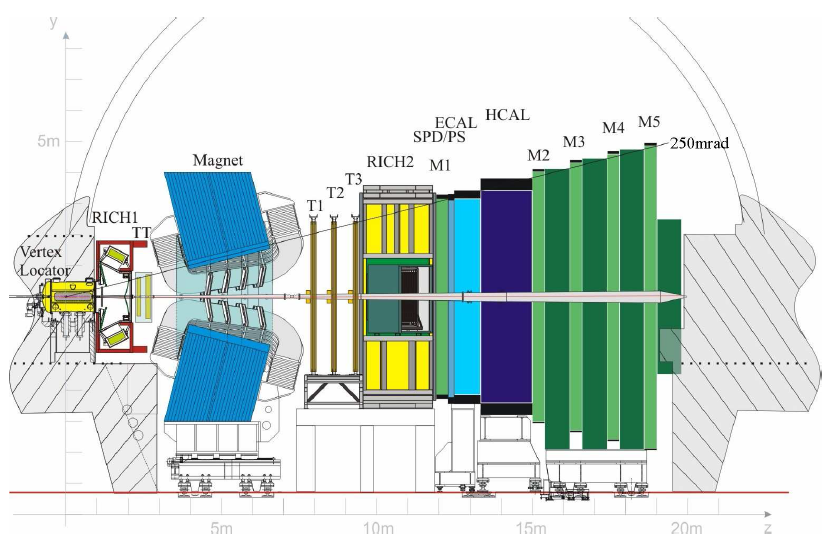
\includegraphics[width=\textwidth]{lhcb-detector}	
	\caption{The \lhcb detector.}
	\label{fig:detector}
\end{figure}

% ===========================
% SECTION: Tracking detectors
% ===========================
\section{Tracking detectors}
Tracking describes the whole procedure to reconstruct the trajectories of the (charged) particles produced in the proton-proton collision. If there's a magnet in use, the particles' charges and momenta can be determined as well. For that purpose, a system of several subdetectors is aligned up- and downstream the dipole magnet, namely the Vertex locator (VELO), the Trigger Tracker (TT) and the Trigger stations (T1-T3) built-up by the Inner Tracker (IT) and the Outer Tracker (OT).

\subsection{Vertex Locator (VELO)}
The VErtex LOcator (VELO) is placed directly around the primary interaction point. 
Its task is to precisely measure the track coordinates of charged particles and separate the proton-proton interaction point from other vertices, namely either other primary vertices (so called pile-up events) or secondary vertices. 
The latter ones are typically for \bquark- or \cquark-hadron decays \cite{VELO_TDR} and a good separation and resolution of these vertices is crucial for the \lhcb physics programme.
As an example serves the measurement of particles' decay length and time for the determination of the rapid $\Bs-\Bsb$ oscillation frequency \cite{BsBsbar_frequency}.

The VELO is built up by silicon modules due to the high particle flux and thus high radiation in the interaction region. It is placed only 7\mm apart from the beam. This is closer than the required aperture of the \lhcb beam pipe at injection. Thus, the VELO sensors are made of silicon microstrips shaped as slightly overlapping half-discs. The two halfs can be moved in $x$- and $y$-direction to avoid radiation damages unless the beam is stable.

Each module provides a measurement of the $r$- and $\phi$-coordinates.
The sensores for these measurements are correspondingly called $R$- and $\Phi$-sensor, which can be seen in figure \ref{fig:VELO_RandPhiSensor}.
An overview over the VELO system with its modules is shown in figure \ref{fig:VELO_Overview}. Around the nominal interaction region, the modules are placed closer to each other. Upstream there are two $R$ sensors dedicated to veto pile-up events. 
Figure \ref{fig:VELO_Overview} furthermore shows the VELO in closed and opened position.
\begin{figure}[hptb]
    \centering
	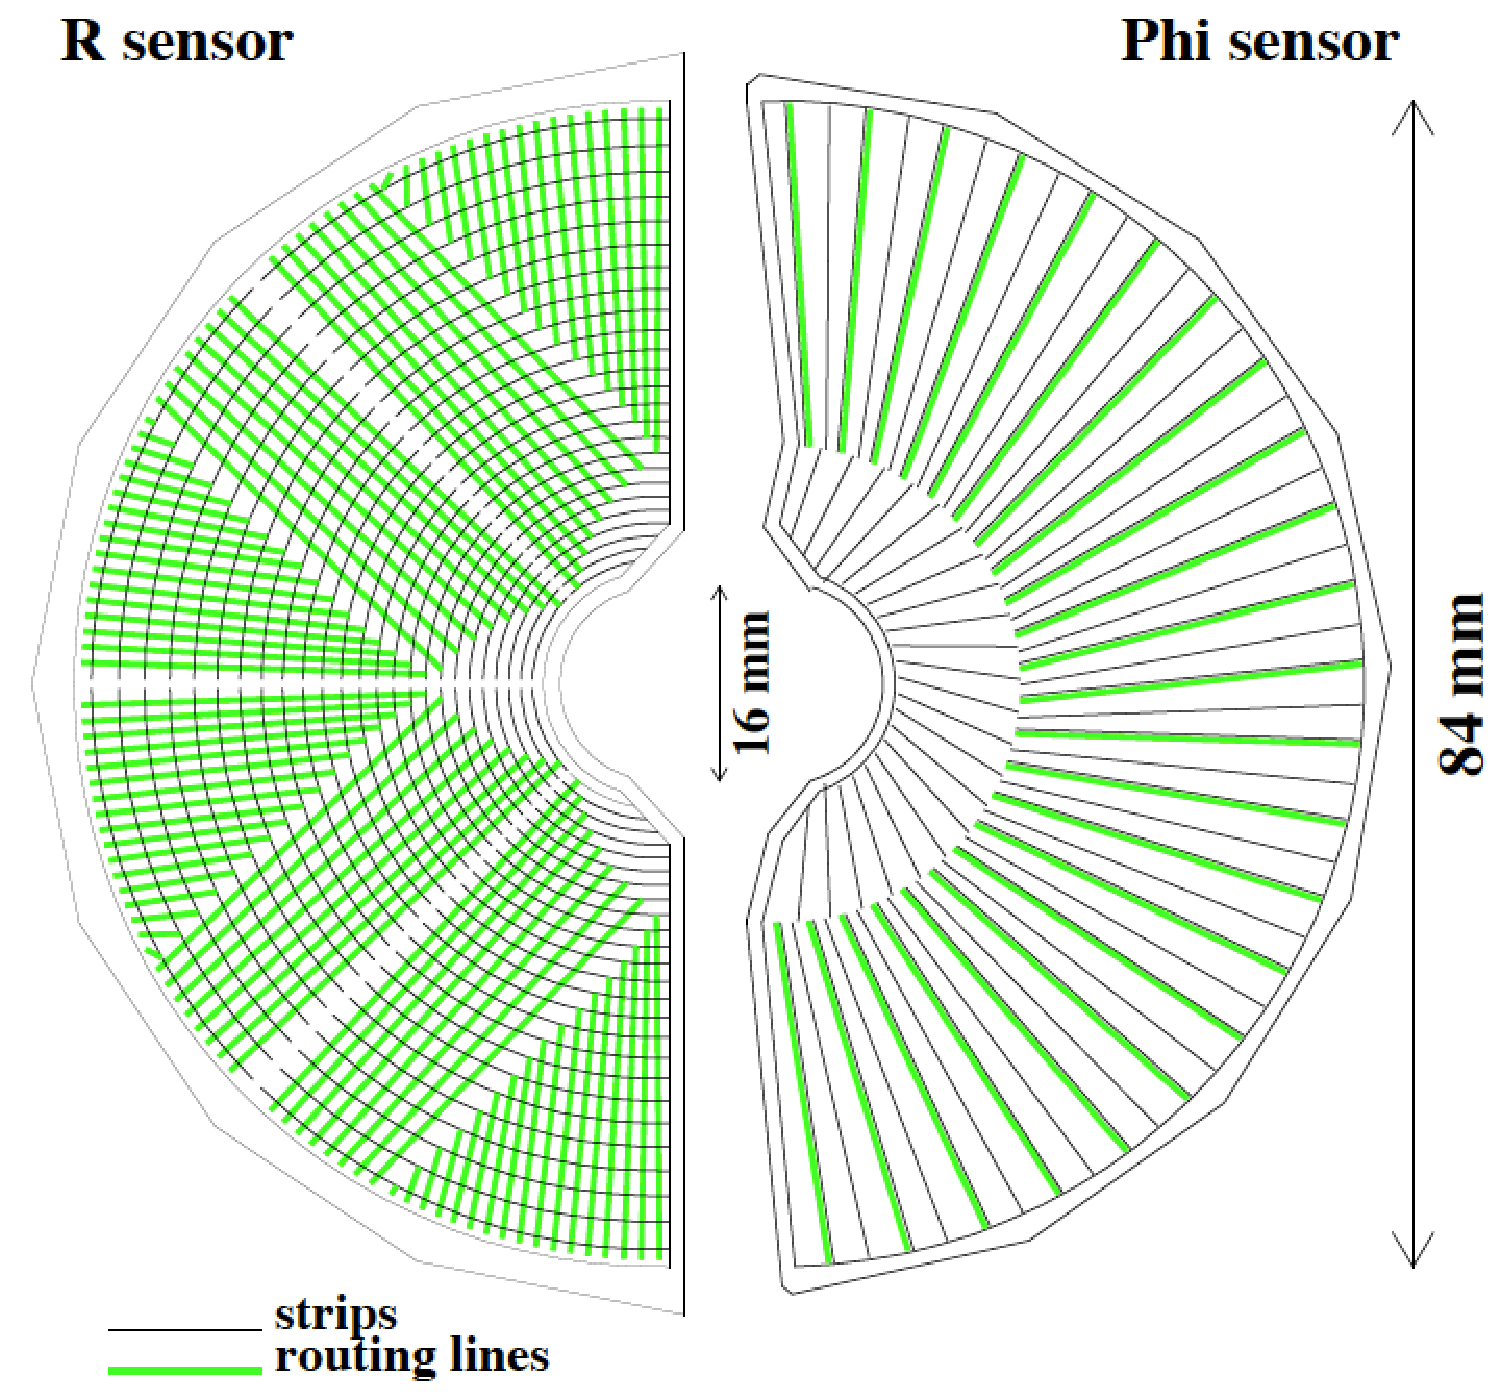
\includegraphics[width=0.5\textwidth]{VELO_randphisensors}	
	\caption{Schematic representation of an $R$ and a $\Phi$ sensor. The $R$ sensor strips are arranged into four approximately 45\degrees segments and have routing lines perpendicular to the strips. The $\Phi$ sensor has two zones with inner and outer strips. The routing lines of the inner strips
    are orientated parallel to the outer strips. Figure and caption taken from \cite{VELO_Performance}.}
	\label{fig:VELO_RandPhiSensor}
\end{figure}
\begin{figure}[hptb]
    \centering
	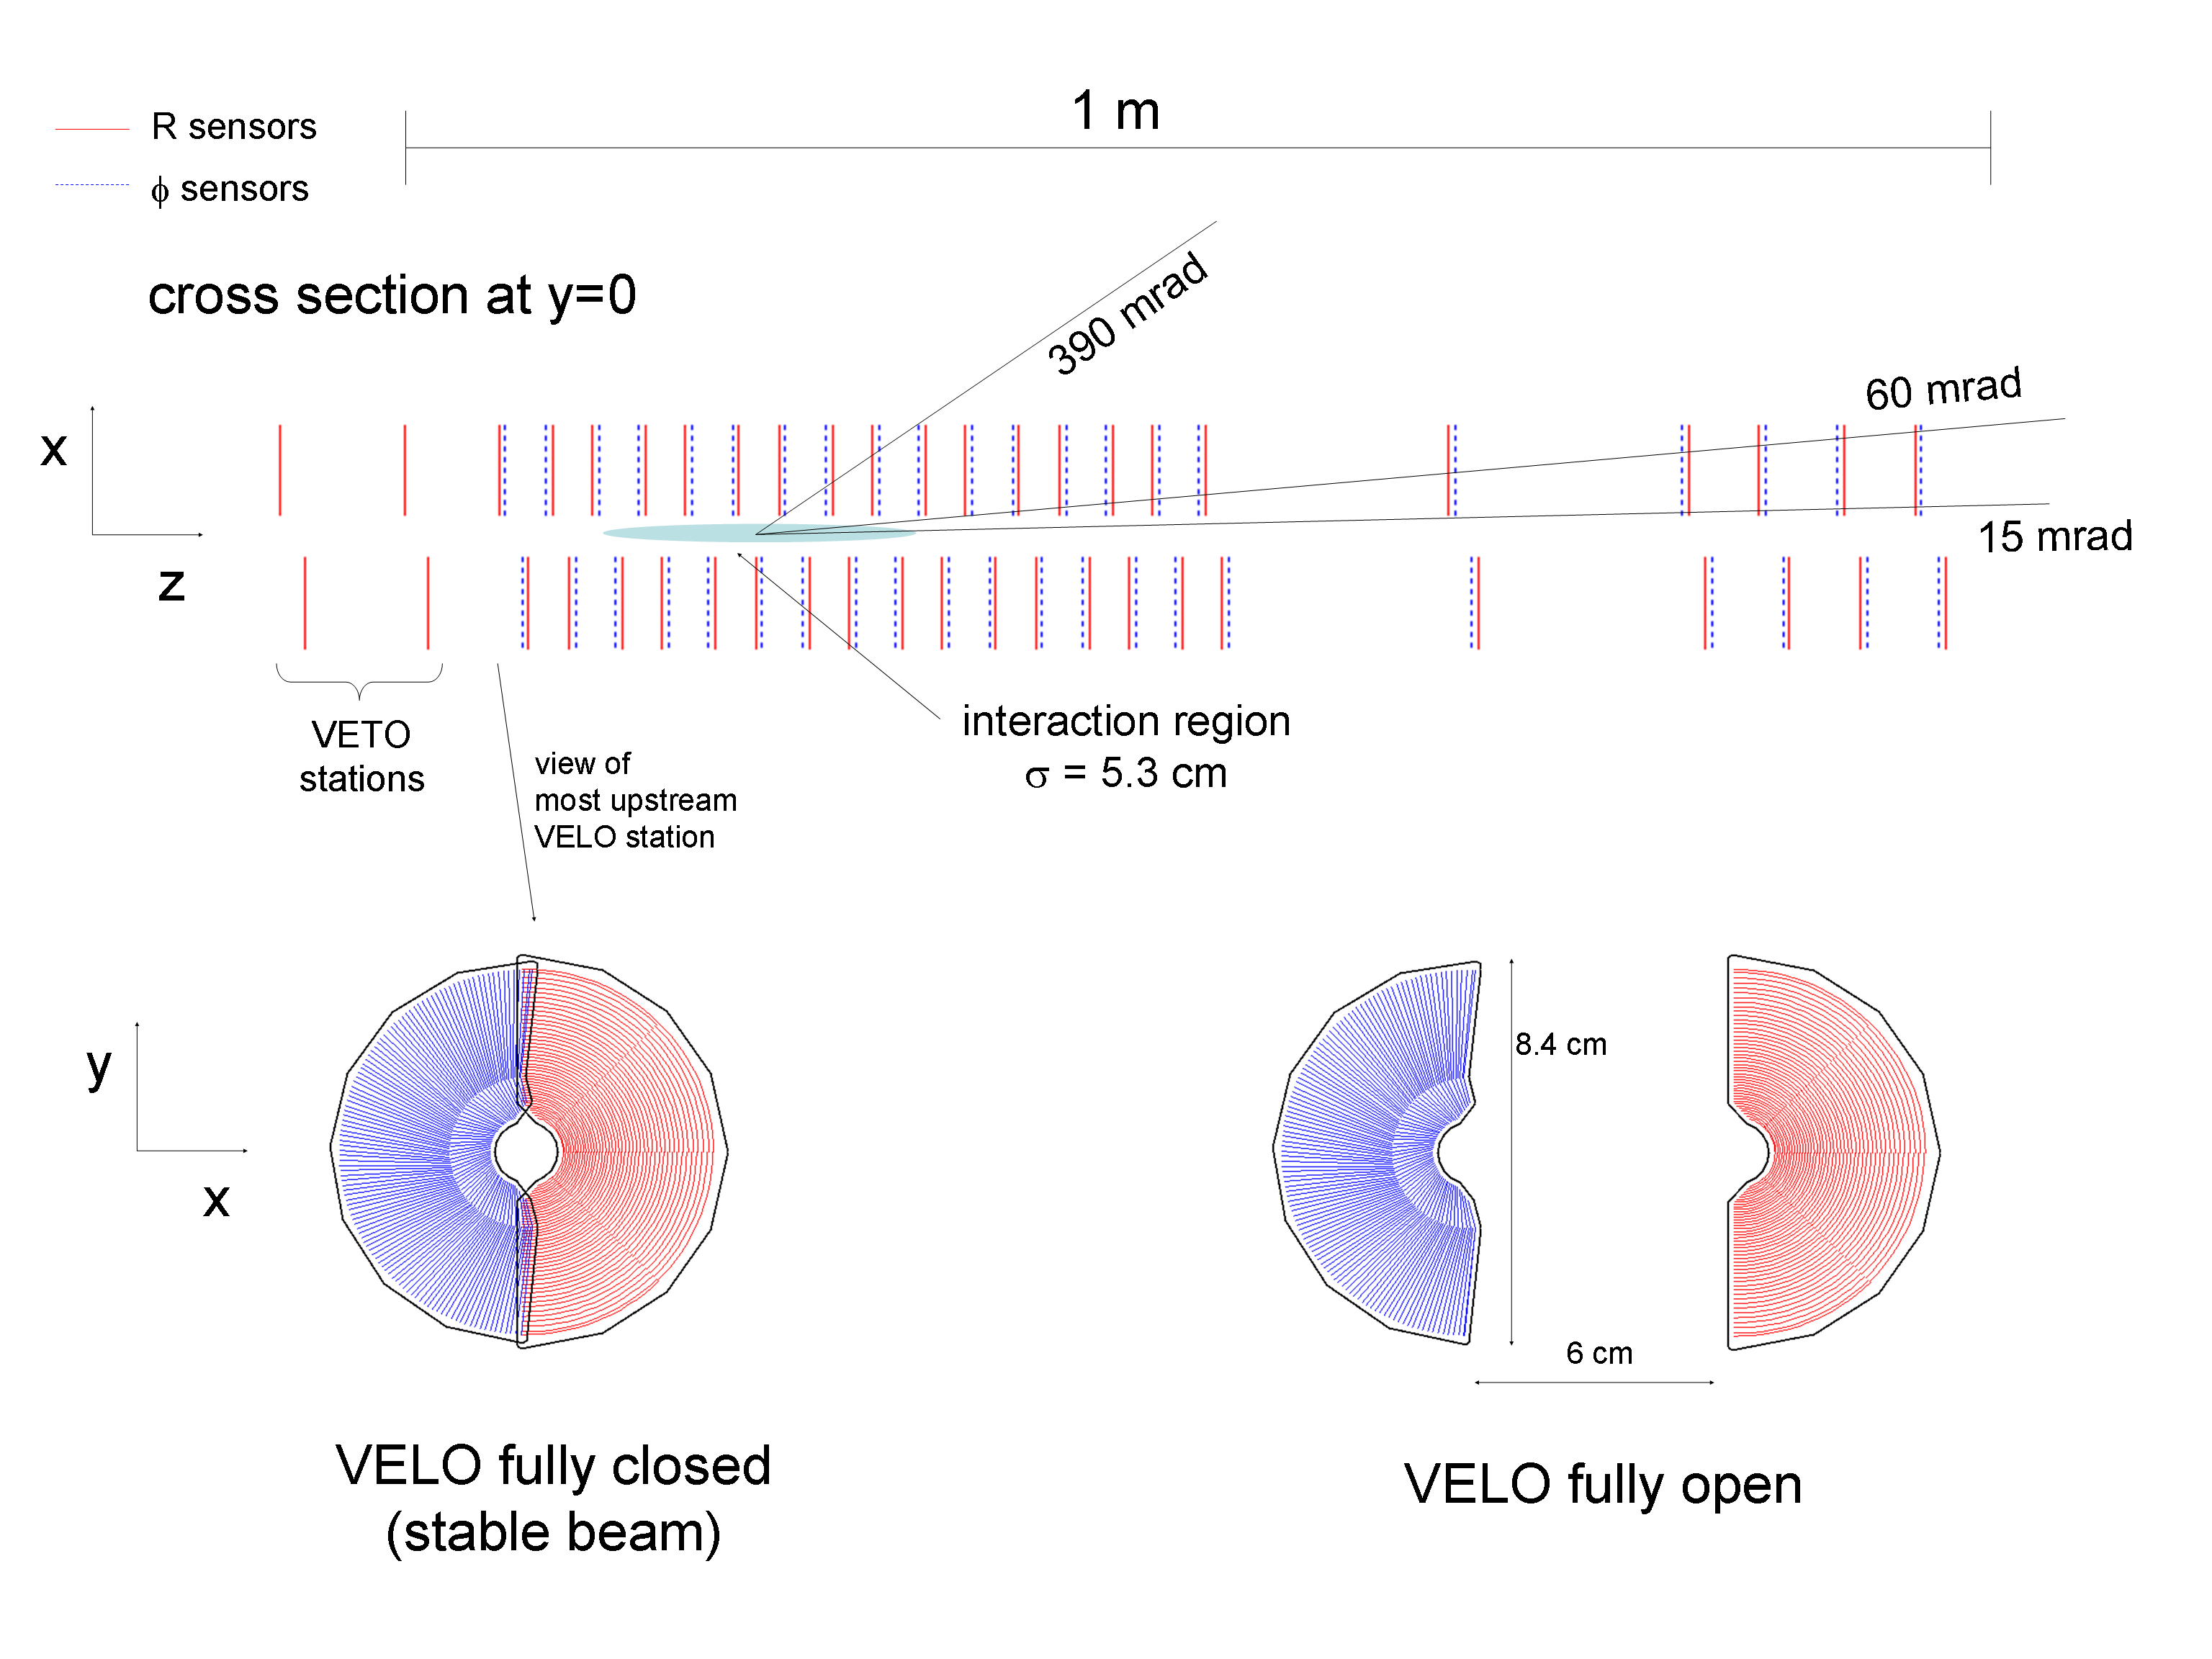
\includegraphics[width=0.8\textwidth]{VELO_Overview}	
	\caption{Cross section in the $(x,z)$ plane of the VELO silicon sensors, at $y=0$, with the detector in the fully closed position. 
             The front face of the first modules is also illustrated in both the closed and open positions. 
             The two pile-up veto stations are located upstream of the VELO sensors.
             Figure and caption taken from \cite{detector}.}
	\label{fig:VELO_Overview}
\end{figure}
With this setup the VELO reaches a track finding efficiency above 98\%. Its resolution on vertices is 13\mum in the transverse plane and 71\mum along the beam axis for vertices with 25 tracks. 
The resolution on the impact parameter is smaller than 35\mum for particles with a transverse momentum larger than 1\gev \cite{detector, VELO_TDR, VELO_Performance}.

\subsection{Trigger Tracker / Tracker Turicensis (TT)}
The Tracker Turicencis or formerly the Trigger Tracker is located in front of the entrance of the \lhcb magnet. It is used for sevaral tasks:
\begin{itemize}
    \item deliver transverse momentum information for Level-1 trigger,
    \item reconstruct trajectories of long-lived neutral particles decaying outside the VELO
    \item reconstruct low-momenta particles bent out by the magnet before reaching the station T1-T3.
\end{itemize}

The TT makes completely use of silicon microstrip detector. It consist of one station made of four planes along the beam axis. The first and the fourth layer have vertical readout strips ($x$-layer), while the second and third are rotated by an angle $\pm 5\degrees$ to get a high resolution in the
bending plane and additional information in $y$-direction.
Between the $u$ and $v$ layer there is a gap of around 30\cm. Figure \ref{fig:TT_layers} shows schematically the layout of the TT.
\begin{figure}[hptb]
    \centering
	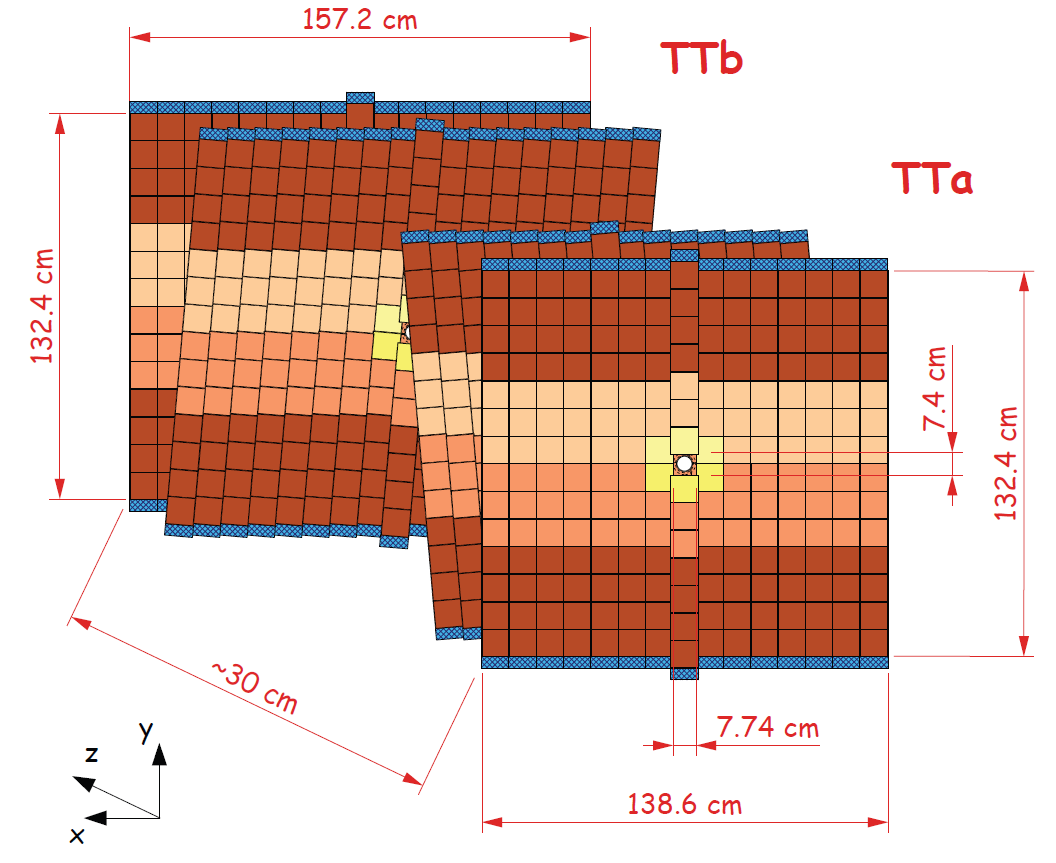
\includegraphics[width=0.8\textwidth]{TT_layers}	
	\caption{Layout of the Tracker Turicensis (TT). 
             Figure taken from \cite{ST_Performance}.}
	\label{fig:TT_layers}
\end{figure}

\subsection{Inner Tracker (IT)}
Being a silicon micro-strip detector, the Inner Tracker (IT) uses the same technology as the TT. 
It builds the inner part of the three tracking stations T1-T3 (see figure \ref{fig:detector}).
Each station consists of four boxes as shown in figure \ref{fig:IT_layer}.
In each box there are again 4 layers, two vertical and two stereo, analogously to the TT \cite{detector, ST_Performance}.
\begin{figure}[hptb]
    \centering
	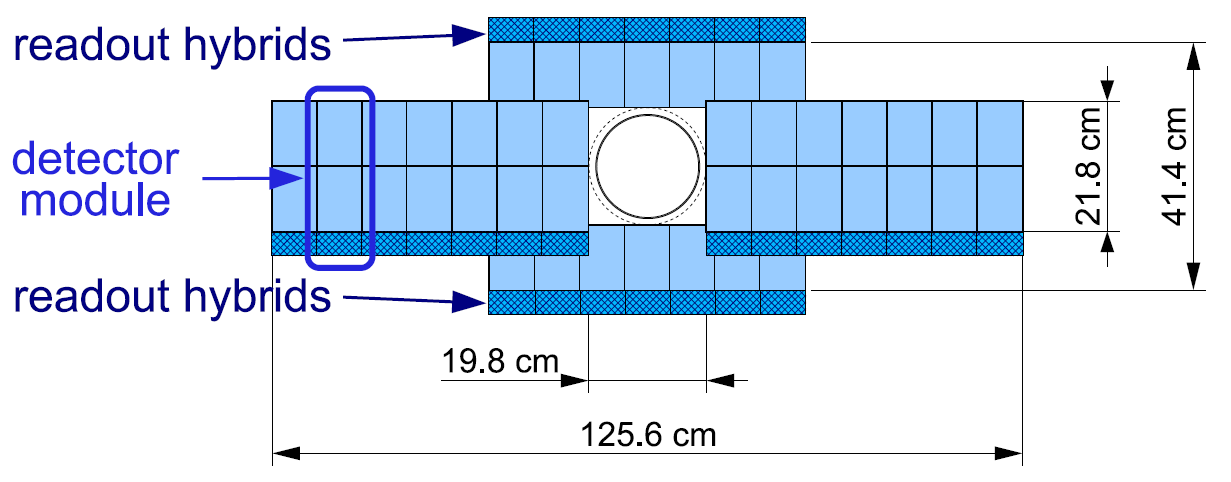
\includegraphics[width=0.8\textwidth]{IT_layer}	
	\caption{Layout of a $x$ detection layer in the second Inner Tracker (IT) station. 
             Figure taken from \cite{detector}.}
	\label{fig:IT_layer}
\end{figure}

\subsection{Outer Tracker (OT)}

\subsection{Track classification}


% ================================
% SECTION: Particle identification
% ================================
\section{Particle identification}

\subsection{Ring Imaging Cherenkoy Detector (RICH)}

\subsection{Calorimeter system}

\subsection{Muon chambers}

% ===========================
% SECTION: Trigger
% ===========================
\section{Trigger}

\subsection{L0-Trigger}

\subsection{High Level Trigger (HLT)}

	%\chapter{Theory and motivation}
\label{sec:Theory}

\section{The Standard Model of Particle Physics}
The Standard Model of particle physics (SM) is a relativistic and renormalisable quantum field theory, that combines the electroweak theory developed by Glashow, Salam and Weinberg \cite{SM_Glashow, SM_Salam, SM_Weinberg} with quantum chromodynamics (QCD), the theory of the strong interactions.
It combines the current knowledge of fundamental particles and their interactions at microscopic level with the exception of gravitation.

The electroweak theory is already a combination of the electromagnetic and the weak interaction.
Every fundamental particle can interact via the weak force.
For instance, the weak force is responsible for the $\beta$-decay of neutrons.
Atoms or molecules are bound by the electromagnetic interaction taking place between electrically charged particles.
If particles also carry a so-called colour charge, they can interact via the strong interaction, which binds e.g. protons and neutrons in a nucleus.

In the Standard Model, matter arises as half-integer spin particles from quantum fields.
These particles are called \textsc{Fermions} and can be furthermore split up in \textsc{Quarks} and \textsc{Leptons}.
There exist 6 so-called ``flavours" of quarks: up (\uquark), down (\cquark), charm (\cquark), strange (\squark), top (\tquark) and bottom\footnote{The bottom quark is sometimes also called beauty.} (\bquark).
According to their mass and other physical properties, they can be grouped into three generations:
\begin{align*}
    \begin{pmatrix} \uquark \\ \dquark \end{pmatrix},
    \begin{pmatrix} \cquark \\ \squark \end{pmatrix},
    \begin{pmatrix} \tquark \\ \bquark \end{pmatrix}.
\end{align*}
Quarks in the top row are referred to as \textsc{Uptype} quark.
They carry an electrical charge of $+\frac{2}{3}e$, whereas \textsc{Downtype} quarks carry a charge of $-\frac{1}{3}e$.
Thus, they can participate in the electromagnetic interaction.
In addtion, quarks carry colour charge allowing them to interact via the strong interactions.

Leptons do not carry flavour as opposed to quarks.
There exist three flavours of leptons, namely the electron (\en), the muon (\mun) and the tauon (\taum) with an electric charge of $-e$ and their neutral counterparts, the neutrinos \neue, \neum, \neut.
Similarly to quarks, the leptons can be grouped into three generations
\begin{align*}
    \begin{pmatrix} \en \\ \neue \end{pmatrix},
    \begin{pmatrix} \mun \\ \neum \end{pmatrix},
    \begin{pmatrix} \taum \\ \neut \end{pmatrix}.
\end{align*}
As the neutrinos do neither carry electrical nor colour charge, they only interact weakly.
Due to that fact it is not possible to detect neutrinos at hadron colliders like the \lhc.
For each fermion, there exists a corresponding antifermion with same mass, but opposite quantum numbers.

In the Standard Model, the interactions among the particles are described by the mediation of spin-1 gauge bosons.
For the electromagnetic interaction, this is the electric neutral photon \g.
It couples to electrically charged particles.
Since the photon is massless the range of the electromagnetic interaction is infinite.
The weak interaction is mediated by three massive gauge boson.
The electrically charged \Wp and \Wm as well as the neutral \Z boson.
The \Wpm bosons only couple to left-handed fermions (or right-handed antifermions), whereas the \Z couples to both, left- and right-handed fermions, but with different strength.
Due to their large mass of $m_{\Wpm} \approx 80 \gev$ and $m_\Z \approx 91 \gev$ the weak interaction is only short-ranged.
The strong interaction is carried by 8 massless gluons.
They couple to particles carrying a colour charge and carry colour itself.
Thus, there is also a gluon-gluon coupling possible leading to a QCD coupling strength \as, which strongly depends on the momentum transfer in an interaction.
For low energies \as increases dramatically, which means that coloured particles cannot be isolated.
This phenomenon is called \textsc{Confinement}.
At high energies \as is very small resulting in the \textsc{Asymptotic Freedom}, i.e. the quarks are thus quasi-free while keeping short distances.
Due to the confinement, \textsc{Hadrons}, strongly interacting composite particle, must always be colour-neutral.
They exist either as quark-antiquark system and are called \textsc{Mesons} or as composite of three quarks and are named \textsc{Baryons}.
Recent \lhcb measurements report the observation of candidates for bound states consisting of 4 quarks (2 quark, 2 antiquarks) \cite{Tetraquark} and also 5 quarks (4 quarks, 1 antiquark) \cite{Pentaquark}.

Contradicting to the properties of the particles mentioned above, the invariance of local gauge transformation requires that the particles of the Standard Model are massless.
This problem is solved by the \textsc{Higgs mechanism}, which introduces a doublet of complex scalar (spin 0) fields.
The potential of thies field spontaneously breaks the electroweak symmetry and leads to massive bosons and fermions due to interaction with the Higgs field.
The Higgs mechanism furthermore predicts a massive spin-0 particle, the \textsc{Higgs Boson}.
As lastly unobserved particle, its discovery in July 2012 by \atlas \cite{Higgs_ATLAS} and \cms \cite{Higgs_CMS} was a big success for the experimental community as well as for the theory of the Standard Model itself. 
Figure \ref{fig:SM} summarises the fermions and bosons of the Standard Model and list their main properties \cite{Perkins_HEP, Burgess_SM, Meissner}.
\begin{figure}[ptb]
    \centering
	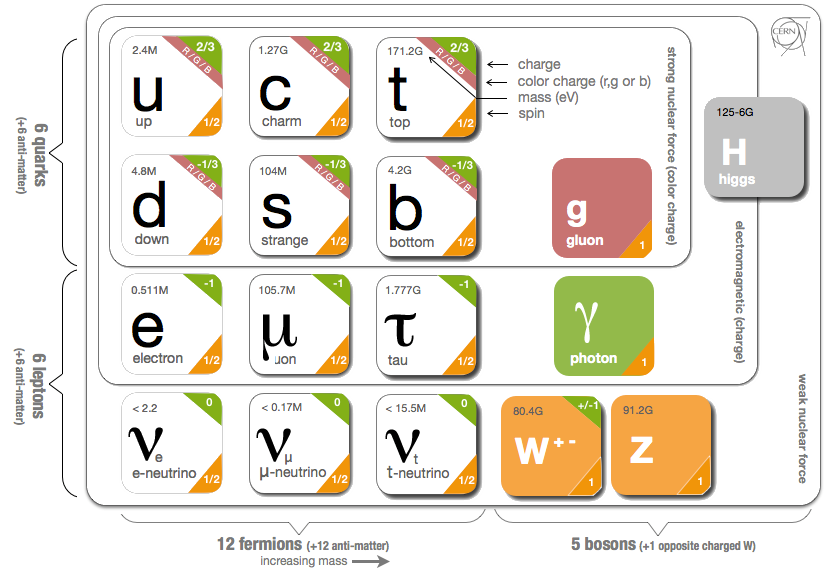
\includegraphics[width=\textwidth]{Standard_Model}	
	\caption{Summary of all fundamental fermions and bosons of the Standard Model of particle physics with their most important properties. Figure slightly modified and taken from \cite{SM_figure}.}
	\label{fig:SM}
\end{figure}

\section{Baryons}

\section{Resonances}

\section{Methods of parameter estimation}
This section briefly describes two methods to estimate parameters, which are used in this thesis.

\subsection{Maximum-Likelihood method}
A common task in High Energy Physics is to find the best estimate for a set of parameters $\vec{\theta}$ by a measurement of some variables $\vec{x}$.
As an example one wants to measure the mass $m_X$  and the width $\Gamma_X$ of a particle $X$ decaying into two daughter particles $A$ and $B$, i.e. $X \to AB$.
For this purpose one would measure the energies $E$ and momenta of $p$ multiple times.
Thus the set of measured variables would be $\vec{x} = (E_A, \vec{p}_A, E_B, \vec{p}_B)$ and one would try to find the ``best" value for the parameters $\vec{\theta} = (m_X, \Gamma_X)$. 
The most frequently used method for the estimate of $\vec{\theta}$ is the \textsc{Maximum-Likelihood Method}.
Given a theoretical prediction of the measured distribution in form of a probability density function $f(\vec{x}|\vec{\theta})$ one can define the likelihood function
\begin{align}
    \mathcal{L}(\vec{x}|\vec{\theta}) := \prod_{i=1}^{N} f(\vec{x}_i|\vec{\theta}),
\end{align}
where $N$ denotes the number of (independent) measurements.
The maximum of this likelihood function $\mathcal{L}$ with respect to $\vec{\theta}$ is assumed to be the best estimate of $\vec{\theta}$.
Practically one minimises equivalently $-\log(\mathcal{L})$ for computational reasons.

Often, a probability density function $P$ is a linear combination of several components, e.g. a signal and background component $P_\text{sig}$ respectively $P_\text{bkg}$.
Thus the number of events $N$ is a random variable as well.
If $N$ obeys the Poisson distribution the so-called \textsc{Extended Likelihood Function} can be defined as: 
\begin{align}
    &\mathcal{L}_\text{ext}(\vec{x} | \Nsig, \Nbkg, \vec{\theta}) :=  \nonumber \\ 
    &\qquad \frac{(\Nsig+\Nbkg)^N\exp{(\Nsig+\Nbkg)}}{N!} \prod_{i=1}^{N} \left[f_\text{sig}P_\text{bkg}(\vec{x}_i|\vec{\theta}) + f_\text{bkg}P_\text{bkg}(\vec{x}_i|\vec{\theta})\right],
\end{align} 
where $N_j$ denotes the corresponding yield and $f_j:=\frac{N_j}{N}$ the fraction of signal respectively background component.
Thus the maximisation of the extended likelihood function $\mathcal{L}_\text{ext}$ enables to estimate the yields of each component at the same time \cite{Lista_Statistics, PDG}.

\subsection{Beeston-Barlow method}
\label{sec:BeestonBarlow}
When one tries to estimate the composition of a data sample it might happen that there does not exist an analytic form of the distribution.
Thus, one relies on simulations and has to bin the data into $n$ bins.
This gives a set of numbers ${d_i}$ with $i \in [1,n]$, where $d_i$ denotes the number of data events in falling into bin $i$.
Let $j$ denote a source contained in the data, $P_j$ its strength and $a_{ji}$ the number of simulated events from source $j$ in bin $i$, then the predicted number of events in bin $i$ is given by
\begin{align}
    f_i := N_\text{D} \sum_{j=1}^{m} \frac{P_j a_{ji}}{N_j},
\end{align}
where $N_\text{D}$ is the total number of events in the data sample, $N_j$ the number of simulated events for source $j$ and $m$ the number of sources.
Starting from a Poisson distributed probability of observing a particular $d_i$ as
\begin{align}
    \mathrm{e}^{f_i} \frac{f_i^{d_i}}{d_i!}
\end{align}
the logarithmic likelihood to be maximised looks like
\begin{align}
    \log \mathcal{L} = \sum_{i=1}^{n} \left[d_i \log(f_i) - f_i\right] \label{eq:BinnedLL}
\end{align}
after dropping the constant factorials.
This likelihood function is also known as \textsc{Binned Likelihood}.

Nonetheless, the binned likelihood of equation (\ref{eq:BinnedLL}) does not account for finite sizes of the simulation samples.
Due to large computation times simulation samples are often small and there are non-negligible statistical fluctuations in the $a_{ji}$.
Thus the likelihood function has to be modified as follows:
The predicted number of events in a bin is now
\begin{align}
    f_i := N_\text{D} \sum_{j=1}^{m} \frac{P_j A_{ji}}{N_j},
\end{align}
where $A_{ji}$ is the unknown expected number of events for source $j$ in bin $i$.
The ``observed" $a_{ji}$ in the simulation sample is generated from $A_{ji}$ by a Poisson distribution\footnote{Actually, the $a_{ji}$ obey a binomial distribution. However, for $A_{ji} << N_j$ it can be approximated by a Poisson distribution.}.
Thus, the probabilities of observing a set of ${d_i}$ and ${a_ji}$ have to be combined and the likelihood function to be maximised is
\begin{align}
    \log \mathcal{L} = \sum_{i=1}^{n} \left[d_i \log(f_i) - f_i\right] + \sum_{i=1}^{n} \sum_{j=1}^{m} \left[a_{ji} \log(A_{ji}) - A_{ji}\right]. \label{eq:BBLL}
\end{align}
Throughout this analysis, the maximisation of this likelihood function in equation (\ref{eq:BBLL}) is referred to as \textsc{Beeston-Barlow Method} \cite{BeestonBarlow}.

	%\chapter{Data reconstruction and selection}
\label{sec:Selection}
The data sample used in this analysis originates from \proton\proton collisions and has been recorded in the years 2011 at a center of mass energy $\sqs = 7 \tev$ and 2012 with $\sqs = 8 \tev$, corresponding to an integrated luminosity of \intlum{3 \invfb}.
This chapter describes and motivates the selection criteria for the reconstruction of the decays \LbToDpmunuX and \LbToLcmunu\footnote{If not stated otherwise, the $\mathcal{CP}$ conjugated decays \decay{\Lbbar}{\Dzb\antiproton\mup\neum} and \decay{\Lbbar}{\Lcbar\mup\neum} are included in those samples}.
As the \Dz and the \Lc are not stable enough to be directly indentified and detected, the subsequent decays \DToKpi and \LcTopKpi have been chosen for their reconstruction.
These decays leave a clear signature in the detector and can be well reconstructed at \lhcb, meaning that the pollution with background is small.
Furthermore, with this choice one ends up with the same final state particles for reconstruction in both signal and normalisation channel, namely \pKpi\mun.
Hence, any inefficiencies due to different interaction of particles with the detector should cancel, at least to first order.

One experimental difficulty arises due to the semileptonic nature of the signal and normalisation channel:
The neutrino cannot be reconstructed.
Consequently it is not possible to fully reconstruct the \Lb and to get a \Lb mass peak for the distinction between signal and background.
This leads to a high pollution of the data sample with backgrounds.

\section{Reconstruction of the decay \LbToDpmunuX}
The main strategy in the reconstruction process of the decay \LbToDpmunuX is to find events with the signature $\decay{X_{b}}{(\DToKpi) \mun \neumb X}$, where $X_b$ denotes a \bquark-quark containing hadron, first.
Then, the proton track is combined to the \Dz\mun vertex to make a \LbToDpmunuX candidate.
It is apparent that a main source of background will be a \decay{\Bd/\Bp}{\Dz\mun\neumb X} decay, where a random proton is added.
To better understand the selection criteria and the way this \textsc{combinatorial background} is reduced, it might be helpful to have a look at a sketch of a typical \LbToDpmunuX decay in Figure \ref{fig:DecaySketch} left.
\begin{figure}[tb]
	\centering
	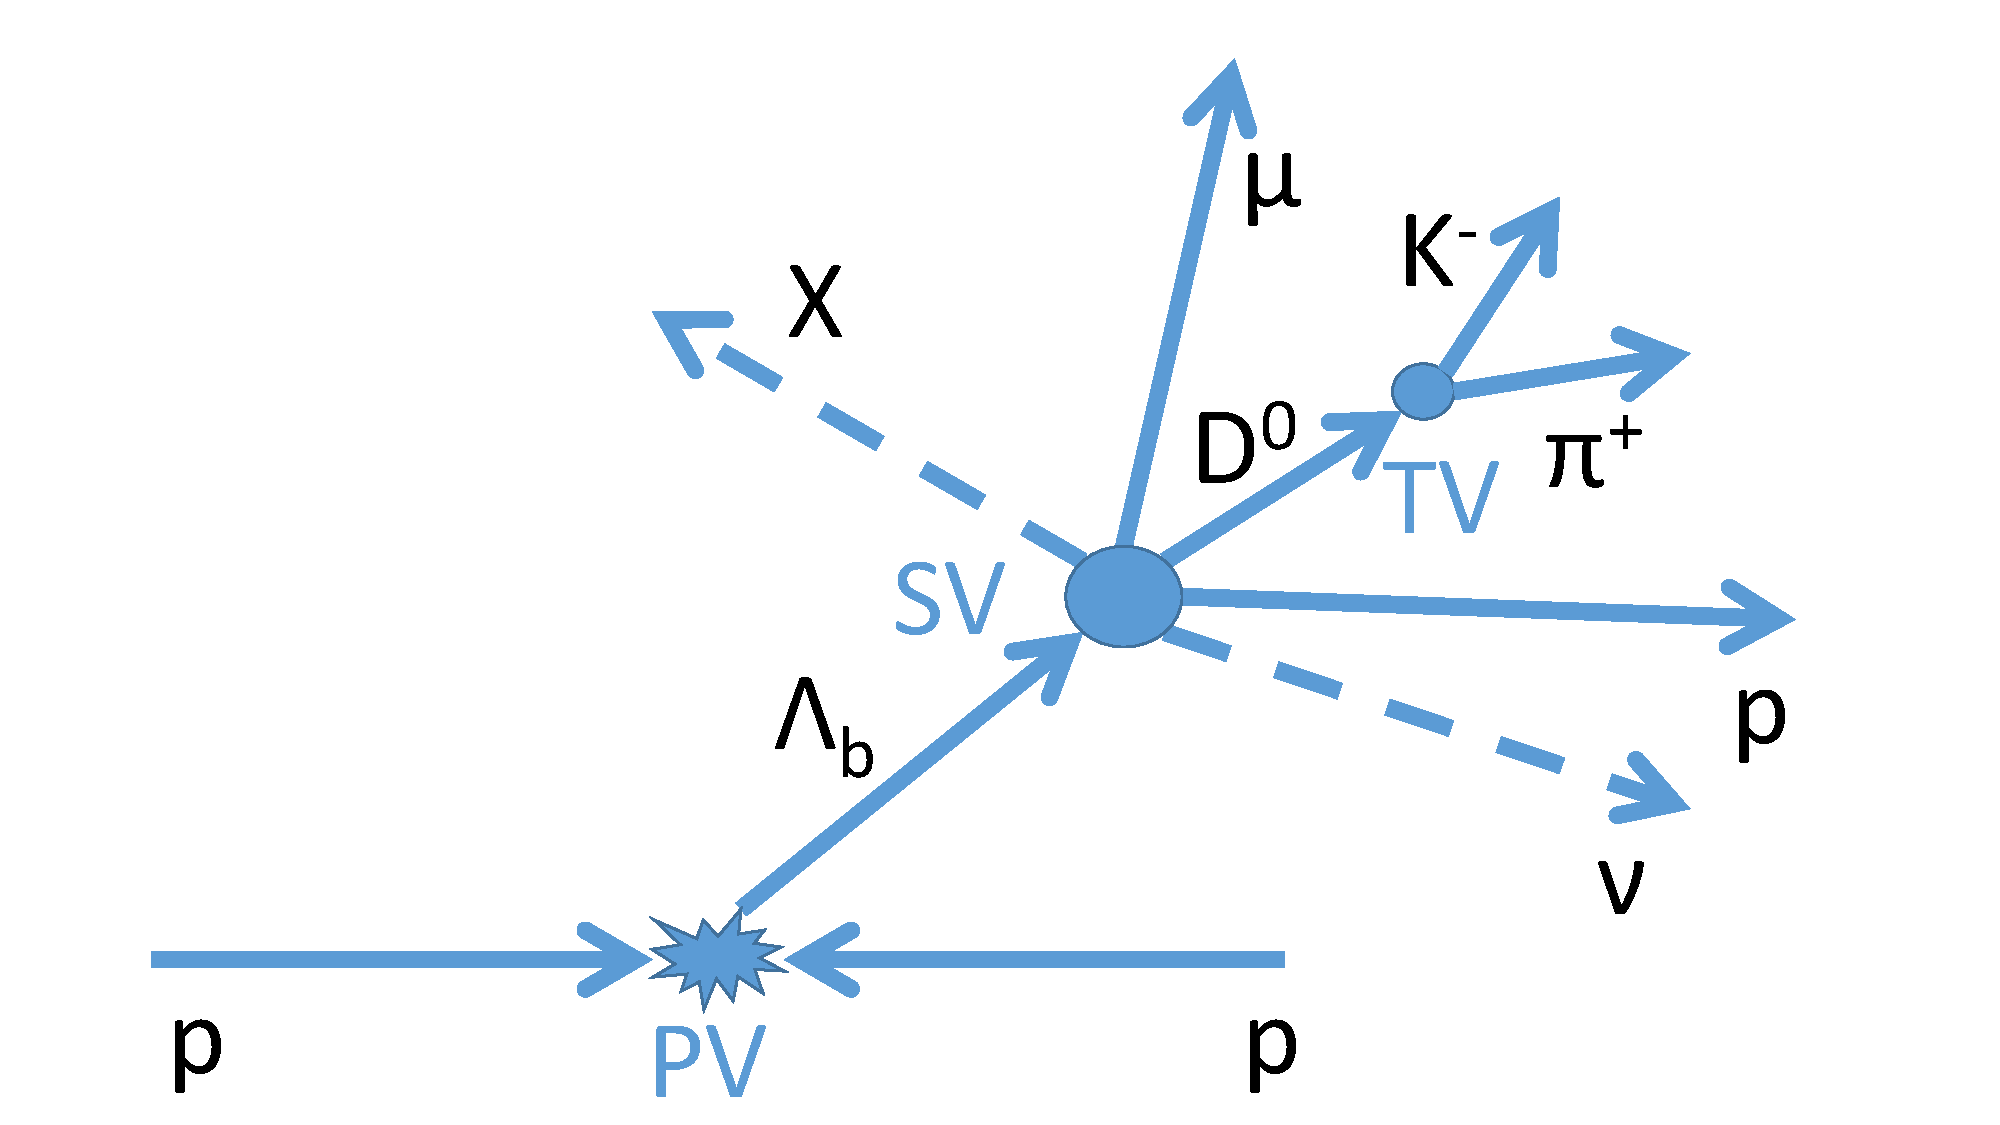
\includegraphics[width=0.49\textwidth]{decay_sketch_signal}
	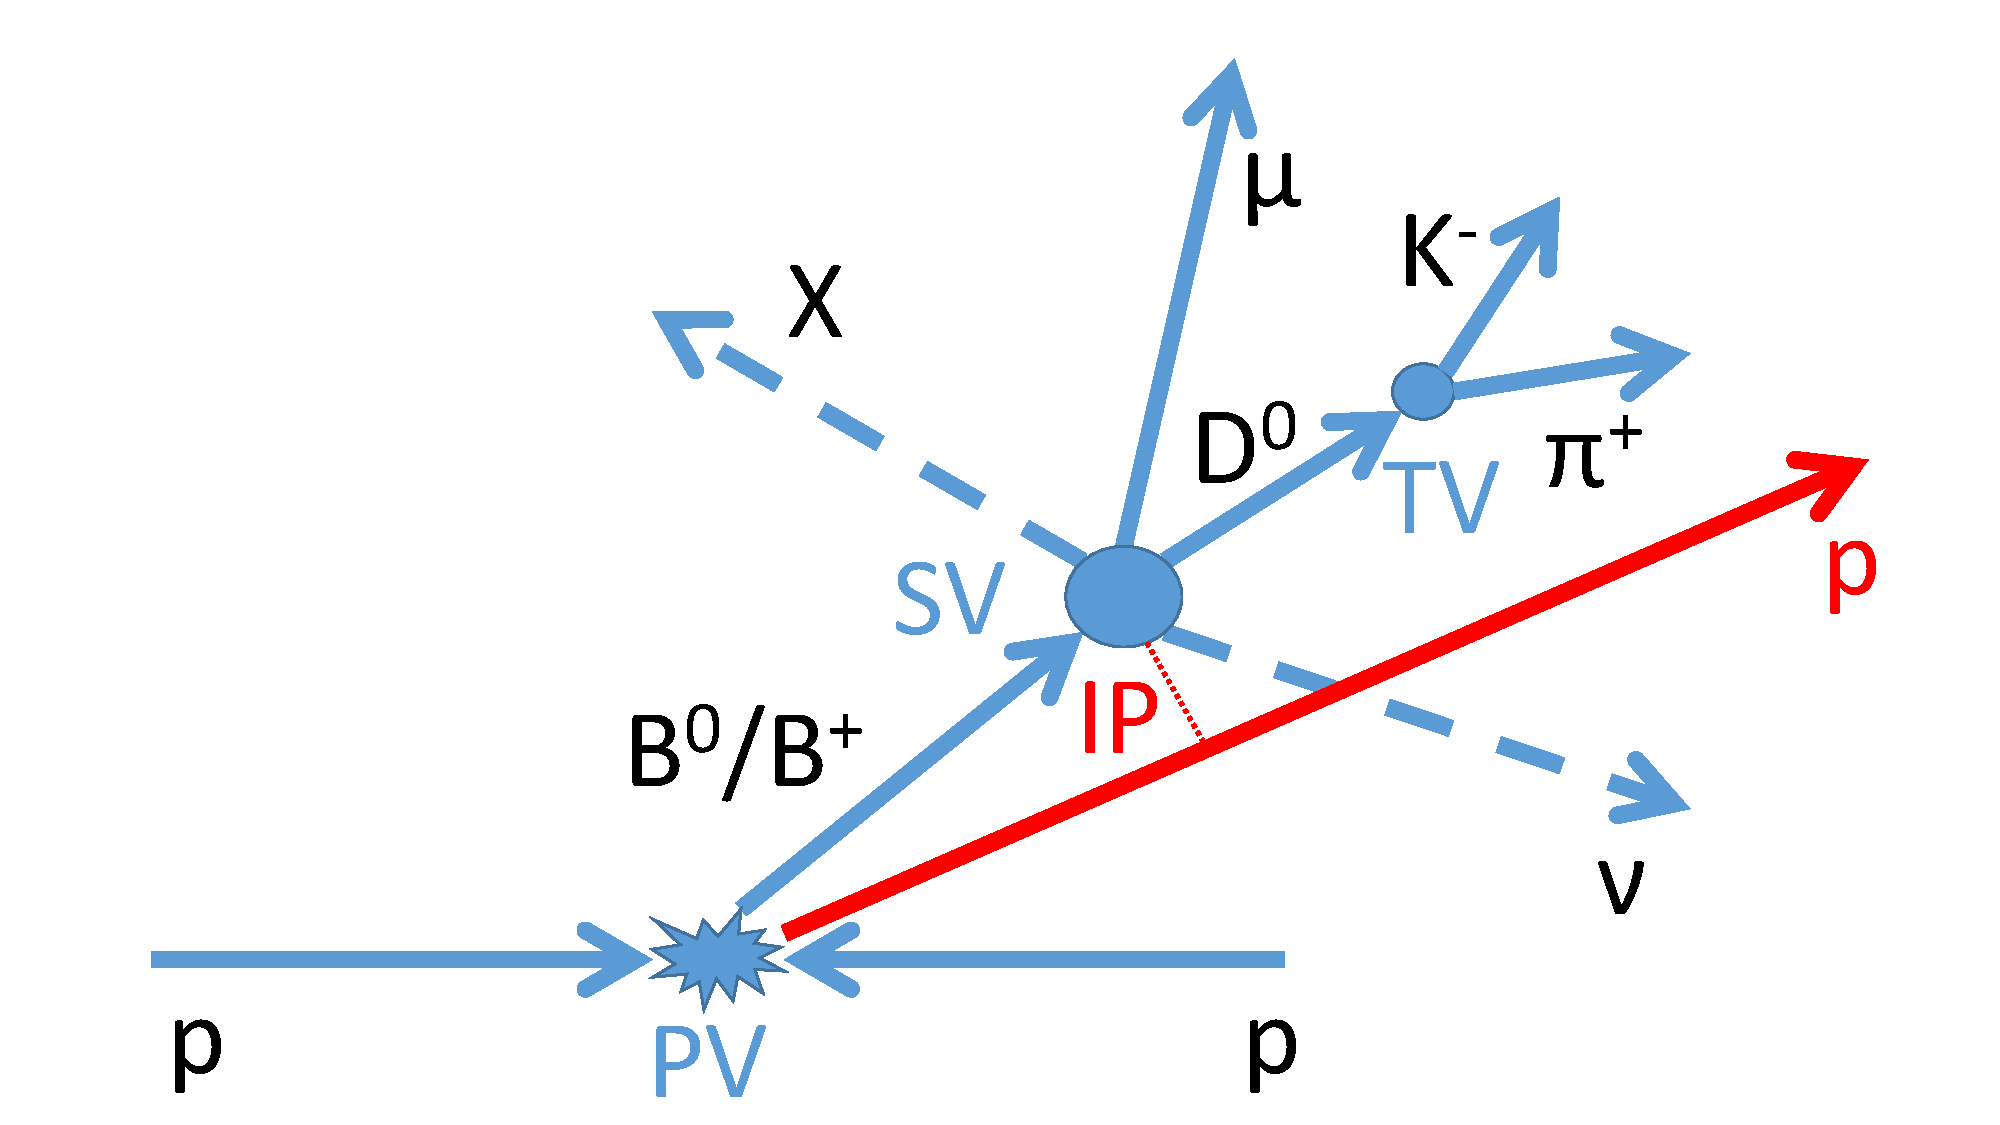
\includegraphics[width=0.49\textwidth]{decay_sketch_background}
	\caption{
        Sketch of the decay topology for a typical \LbToDpmunuX decay (left) and for the background decay \decay{\Bd/\Bp}{\Dz\mun\neumb X} with a randomly combined proton (right).
        In these background events the proton rather poorly makes a vertex with the \Dz\mun candidate, indicated by a large impact parameter (IP).
        Particle tracks drawn with a dashed line are not reconstructed.
        This sketch does neither account for the correct distances between the vertices nor the boost of the particles in $z$-direction.
    }
	\label{fig:DecaySketch}
\end{figure}
Due to its relatively long lifetime, it is typical for a \Lb or in general a \bquark-hadron that it decays at a so called \textsc{secondary vertex (SV)} displaced from the primary \proton\proton interaction, the \textsc{primary vertex (PV)}.
The decay products \Dz, \mun and \proton  originate from the secondary vertex. 
The neutrino and further possible (especially neutral) particles like pions, denoted as $X$, are not reconstructed.
The \Dz itself lives long enough to decay into a \Km\pip at a \textsc{tertiary vertex (TV)}.

Concerning the combinatorial background \decay{\Bd/\Bp}{\Dz\mun\neumb X} with a randomly added proton, there is one important difference to the signal.
The proton does not orgin from the secondary vertex but from another source.
It should thus have a significant \textsc{impact parameter (IP)} with respect to the primary vertex.
The impact parameter is defined as the smallest perpendicular distance between a track and a vertex.
An equivalent way is to use the \logIP variable of a given track with respect to a given vertex, which will be very important throughout this analysis.
All reconstructed track and vertices are fitted in \lhcb.
From each fit one can retrieve the fit \chisq and the corresponding number of degrees of freedom (ndf).
The \logIP of the proton is defined as the logarithm of the difference of the \Dz\mun vertex fit \chisq with and without the proton.
This means the better the proton makes a vertex with the \Dz\mun, the smaller is \logIP and the more likely the event is a real \LbToDpmunuX decay.

\subsection{Reconstruction of the \Dz candidate}
\label{sec:Selection_D0}
The first step of the reconstruction process is to reconstruct the \Dz.
This is supposed to happen via the \DToKpi signature.
For both, kaon and pion, it is required that their momentum is larger than 2 \gev to ensure that they are not bent out of the detector by the magnet and that the \rich detector gives reliable results for the particle idenitification.
Their transverse momentum is required to be larger than 300 \mev.
This suppresses kaons and pions from the primary interaction, which are usually boosted along the beam pipe, thus having a small transverse momentum.
Aside a good track quality quantified with $\chisqndf < 4$ of the track fit, only tracks with a $\chisqip/\text{ndf} > 4$  with respect to the primary vertex are selected, meaning the kaons and pions are not coming from the primary interaction.
\lhcb's particle identification system provides a likelihood for a particle hypothesis of each particle candidate.
For the pion candidate a likelihood is available that it is really a pion or that is a kaon and so on.
One defines the PIDx variable of a particle candidate, which denotes the difference of the logarithmic likelihoods between the hypotheses that this particle is of species x and a pion, i.e.
\begin{align}
    \text{PIDx} = \ln \mathcal{L}_x - \ln \mathcal{L}_\pion, \label{eq:PIDdef}
\end{align}
where $\mathcal{L}_{\pion}$ denotes the likelihood for the pion hypothesis and $\mathcal{L}_{x}$ for particle $x$ respectively.
The higher PIDx the more likely the candidate is really a particle x\footnote{Throughout this thesis x is either mu for muons, p for protons and K for kaons.}.
For the kaon candidate a PIDK $>4$ and for the pion candidate a PIDK $<10$ is required.
At first glance it might be confusing why the requirement on the pion's PIDK is so loose.
In a \proton\proton collision there are many more pions produced than kaons.
Thus it is much more likely that a pion is misidentified as a kaon and the requirement on the PIDK needs to be tight.
However, for pions most of the background are pions, too.
Hence, there is less motivation to apply requirements on the pion PID.
The pion and kaon candidates and their tracks are now combined to a \Dz candidate with a good vertex quality of \chisqvtx/ndf $<6$.
Another variable one defines for the reconstruction is DIRA.
It is defined as the cosine of the angle $\alpha$ between the direction of flight of a particle from some reference vertex and its momentum.
If the detector resolution was perfect, DIRA would be one ($\alpha = 0$).
Requiring a DIRA close to one ensures that the assigned momentum and flight direction match to each other.
The flight direction is determined by the connection of the reference vertex and the decay vertex of the particle.
Throughout this selection, all DIRA requirements are calculated with respect to the primary vertex.
Thus, the DIRA requirements on particles not coming from the primary vertex like the \Dz in this case have to be a bit looser as e.g. for the \Lb which is directly produced at the primary vertex.
For the reconstruction of the \Dz events with a DIRA $>0.99$ of the \Dz are selected.
As last requirement one suppresses combinatorial background by restricting the \Dz to be close to its mean mass, i.e. the mass difference to the PDG value is smaller than 25 \mev and to require a minimum \Dz flight distance with respect to the primary vertex of 5 \mm.
Figure \ref{fig:plot_mD0} shows the invariant mass of the reconstructed \Dz candidates after the application of all the requirements except for the restriction of the \Dz mass itself.
A clear mass peak with very small sidebands indicating a small combinatorial background contribution can be seen.
\begin{figure}[tb]
	\centering
	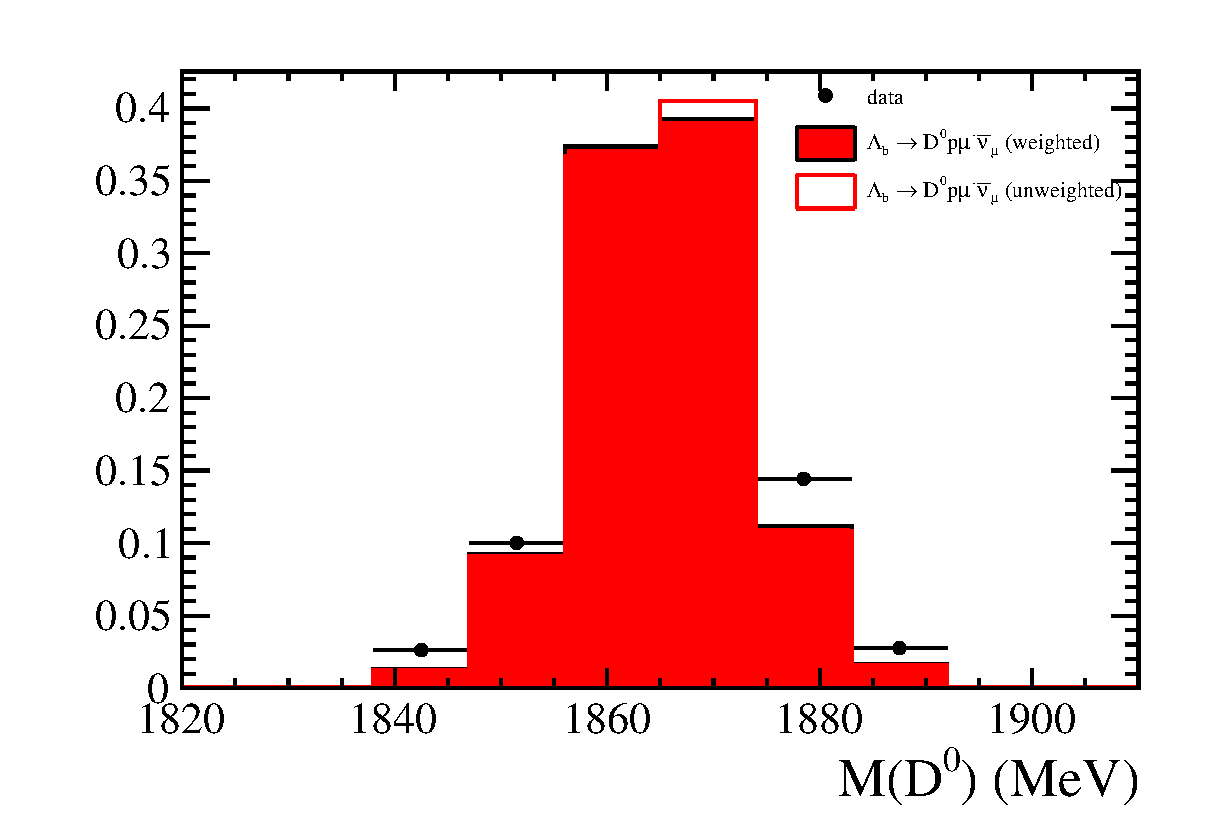
\includegraphics[width=0.8\textwidth]{LbToD0p/plots/data/D0_M}
	\caption{Invariant \Dz mass after the application of all selection requirements except for the \Dz mass itself.
             The arrows indicate where the selection requirements are applied.
             The colour-shaded areas shows the respective distributions for wrong sign (WS) combinations.
             A definition and explanation of wrong sign combinations is given at the end of section \ref{sec:Selection_D0pmu}}
	\label{fig:plot_mD0}
\end{figure}

\subsection{Reconstruction of the \Dz\mun candidate}
\label{sec:Selection_D0mu}
Having reconstructed the \Dz candidate one needs a muon track to combine them.
The motivation for the requirements on the muon track is analagous to the kaon and pion for the \Dz reconstruction.
Thus they will be just briefly mentioned:
The muon is required to have a minimum transverse momentum of 1.2\gev and a minimum momentum of 6\gev.
The track \chisqndf is smaller than 4 and the \chisqip with respect to the primary vertex larger than 9.
PIDmu is required to be greater than 0.3.
It might happen, that several hits in the detector are incidentally combined to a track albeit coming from different tracks.
The so called ghost probablity gives a measure of this issue and is required to be less than 0.5 for the muon track.

For the combination of \Dz and \mun the vertex shall be again of good qualitiy, i.e. \chisqvtx/ndf $<3$.
To avoid completely random combinations the invariant \Dz\mun mass is required to be between 2.2 and 8.0 \gev and a minimum transverse momentum of 3 \gev.
The minimum DIRA of the \Dz\mun candidate is 0.999.
With a requirement on the flight distance \chisq to be greater than 25 it is ensured that the \Dz\mun decay vertex is certainly displaced form the primary vertex.

\subsection{Reconstruction of the \Lb (\Dz\mun\proton) candidate}
\label{sec:Selection_D0pmu}
The proton's momentum and transverse momentum is required to be larger than 15 \gev and 1 \gev respectively for a good particle identification and to exclude protons boosted from the primary interaction.
To reduce the amount of fake protons, i.e. pions or kaon that are misidentified as protons, tight particle idenitification requirements are applied: PIDp $> 10$ and PIDp$-$PIDK $> 10$.
Having the definition of the PIDx variable in equation \ref{eq:PIDdef} in mind, PIDx serves always as distinction between a particle $x$ and a pion.
Thus, the difference between PIDp and PIDK enables for a better distinction between protons and kaons, since
\begin{align*}
    \text{PIDp}-\text{PIDK} &= \left(\ln \mathcal{L}_{\proton} - \ln \mathcal{L}_\pion\right) - \left(\ln \mathcal{L}_{\kaon} - \ln \mathcal{L}_\pion\right) \\
    & = \left(\ln \mathcal{L}_{\proton} - \ln \mathcal{L}_{\kaon}\right).
\end{align*}
The \chisqip with respect to the primary vertex is greater than 25, since the proton must not come from the primary vertex.
In contrast, the proton should make a good vertex with the \Dz\mun candidate.
It is thus required that the \logIP of the proton with respect to the \Dz\mun vertex is smaller than 1.
It should be noted, that throughout this thesis, the simple label \logIP refers to this variable.
This last requirement on \logIP is not applied in the signal fit to distinguish nonresonant signal and background as will be thoroughly explained in chapter \ref{sec:Signalfit}.

For the combined \Dz\mun\proton candidate the requirement on the angle $\alpha$ between flight direction and momentum is the tightest compared to the daughter candidates.
This is obvious since the impact of the detector resolution leading to a discrepancy between flight direction and momentum should be the smallest for the first decay of the decay chain.
An angle $\alpha < 0.015$ is required, which is equivalent to a DIRA $\gtrsim 0.999999$.

As stated at the beginning of this chapter, the information on the neutrino is missing in the reconstruction.
Thus, the reconstructed \Lb mass is smeared out and does not peak at the nominal \Lb mass of 5619.5\mev.
However, there are different ways to at least partially account for the missing neutrino.
One of them is the so called \textsc{corrected mass} of the \Lb.
It is defined as
\begin{align}
    m_{\text{corr}} = \sqrt{m_{\Dz\mun\proton}^2 + p_{\perp}^2} + p_{\perp}, \label{eq:correctedMass}
\end{align}
where $m_{\Dz\mun\proton}$ denotes the invariant mass of the \Dz\mun\proton candidate and $p_\perp$ its transverse momentum perpendicular to the \Lb flight direction, which is measured by the connection of the primary vertex and the \Lb decay vertex \cite{CorrectedMass}.
It is the minimum correction to the \Lb candidate if any daughters are missing.
If only a massless particle is missed the corrected mass would be the mass of the \Lb \cite{HLT2_Topological}.
This can be seen as follows:
In the rest frame of the \Lb, the \Lb mass can be written as
\begin{align}
    m_{\Lb} &= E_{\text{vis}} + E_{\text{miss}} \\
            &= \sqrt{M_{\text{vis}}^2 + p_{\perp, \text{vis}}^2 + p_{\parallel, \text{vis}}^2} + \sqrt{M_{\text{miss}}^2 + p_{\perp, \text{miss}}^2 + p_{\parallel, \text{miss}}^2},
\end{align}
where the index vis denotes the respective quantities of the visible, i.e. reconstructed particles and miss the ones of the missing particles.
If the missing particle is massless and if one changes to the \Lb rest frame, where $p_{\perp, \text{vis}} = p_{\perp, \text{miss}} = p_\perp$ and $p_{\parallel, \text{vis}} = p_{\parallel, \text{miss}} = p_\perp$ the \Lb mass becomes
\begin{align}
    m_{\Lb} = \sqrt{M_{\text{vis}}^2 + p_{\perp}^2 + p_{\parallel}^2} + \sqrt{p_{\perp}^2 + p_{\parallel}^2}.
\end{align}
Furthermore, if the longitudinal momentum can be ignored in the present rest frame the \Lb mass is described by the corrected mass $m_\text{corr}$ \cite{bQuark_LEP, Kodama:1991ij}.
Hence, it is required that the corrected \Lb mass lies around its PDG mass $M(\Lb)=(5619.5 \pm 0.4)\mev$ \cite{PDG} between 5 and 6 \gev.
Figure \ref{fig:plot_correctedMass} shows the distribution of the corrected \Lb mass.
Due to the correction of the missing neutrino it peaks near the PDG mass as explained above.
\begin{figure}[tb]
	\centering
	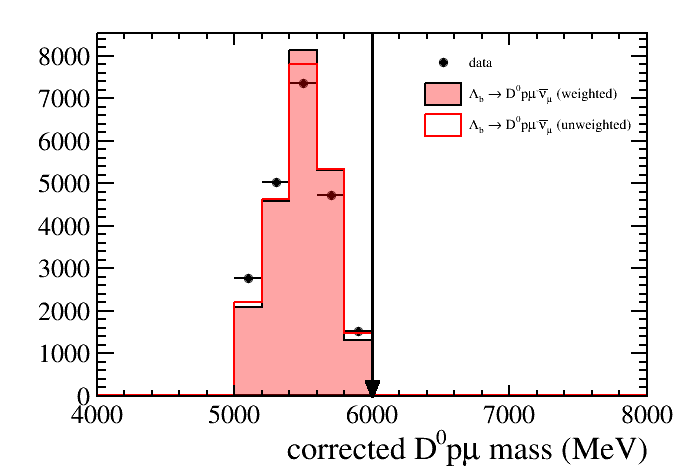
\includegraphics[width=0.8\textwidth]{LbToD0p/plots/data/Bh_BPVCORRM}
	\caption{Corrected \Lb mass after the application of all selection requirements except for the corrected \Lb mass itself.
             The arrows indicate where the selection requirements are applied.
             The colour-shaded areas shows the respective distributions for wrong sign (WS) combinations.
             The corrected \Lb mass tends to peak near the nominal \Lb mass of $M(\Lb)=(5619.5 \pm 0.4)\mev$ \cite{PDG}.}
	\label{fig:plot_correctedMass}
\end{figure}

Another background might be the decay \decay{\Lb}{\Dz\proton\pim}, where the pion is misidentified as muon.
In this case, all final state particles are reconstructed and the invariant \Dz\mun\proton mass peaks around the \Lb mass.
To veto such backgrounds only events with an invariant \Dz\mun\proton mass of less than 5.5 \gev are selected.
A detailed discussion of these backgrounds can be found in chapter \ref{sec:Backgrounds}, especially Figure \ref{fig:plot_D0pmuMass} visualises this veto.

\begin{table}[tb]
    \centering
    \caption{Summary of the selection requirements for the decay \LbToDpmunuX.}
    \label{tab:cuts_D0p}
    \begin{tabular}{r|ll}
        \hline
                & Variable            & Value           \\
        \hline
        Event   
        & number of long tracks       & $< 250$         \\
        \hline
        \mun 
        & Momentum                    & $> 6 \gev$      \\
        & Transverse momentum         & $> 1.2 \gev$    \\
        & Ghost probability           & $< 0.5$         \\
        & Track \chisq/ndf            & $< 4$           \\
        & \chisqip w.r.t. PV          & $> 9.0$         \\
        & PIDmu                       & $> 0.3$         \\
        \hline
        $D^0 \to K^-\pi^+$
        & Daughter momentum           & $> 2 \gev$      \\
        & Daughter transverse momentum& $> 300.0 \mev$  \\
        & Daughter ghost probablity   & $< 0.5$         \\
        & Daughter track \chisq/ndf   & $< 4$           \\
        & Daughter \chisqip w.r.t. PV & $> 4$           \\
        & \Km daughter PIDK           & $> 4$           \\
        & \pip daughter PIDK          & $< 10$          \\
        & \chisqvtx/ndf               & $< 6$           \\
        & DIRA w.r.t. PV              & $> 0.99$        \\
        & Mass difference to PDG      & $< 25 \mev$     \\
        & Flight distance w.r.t. PV   & $> 5 \mm$       \\
        \hline
        $D^0\mun$
        & Mass                            & $\in \left[2.2, 8.0\right] \gev$ \\
        & \chisqvtx/ndf                   & $< 3$                            \\
        & DIRA w.r.t. PV                  & $> 0.999$                        \\
        & Flight distance \chisq w.r.t. PV& $ > 25 $                         \\
        & Transverse momentum             & $ > 3000 \mev $                  \\
        \hline
        \proton
        & \chisqip w.r.t. PV              & $ > 25 $    \\
        & PIDp$-$PIDK                     & $ > 10 $    \\
        & PIDp                            & $ > 10 $    \\
        & Momentum                        & $ > 15\gev$ \\
        & Transverse momentum             & $ > 1 \gev$ \\
        & \logIP w.r.t. \Dz\mun vertex    & $ < 1 $     \\
        \hline
        $D^0\mun\proton$
        & $\arccos$(DIRA) w.r.t. PV       & $ < 0.015 $                   \\
        & Mass                            & $ < 5.5 \gev $                \\
        & Corrected mass                  & $ \in \left[5, 6\right] \gev $\\ 
        \hline
    \end{tabular}
\end{table}

Table \ref{tab:cuts_D0p} summarises all selection requirements mentioned in the last sections.
After the reconstruction and application of these requirements there are in total 21444 \LbToDpmunuX candidates left for the analysis.
In the nominal signalfit the cut on \logIP is not applied.
In this case, there are 34760 candidates available.
Figure \ref{fig:plot_mD0p_logIP} shows the invariant \Dz\proton mass (top) and the \logIP distribution (bottom). 
The first one is used for a spectroscopical analysis later.
If this thesis refers to the \Dz\proton mass, there is rather the quantity $\MDp - M(\Dz) + M_\text{PDG}(\Dz)$, where one first subtracts the reconstructed \Dz mass and then adds up the nominal \Dz mass from the PDG.
With this trick, one ``subtracts" the finite width from the \Dz\proton mass spectrum and improves the mass resolution.
\begin{figure}[tb]
	\centering
	\includegraphics[width=\textwidth]{LbToD0p/plots/data/Bh_DELTA_MASS} \\
	\includegraphics[width=\textwidth]{LbToD0p/plots/data/logIP}
	\caption{Invariant \Dz\proton mass (top) after the application of all selection requirements and \logIP distribution (bottom) after all requirements except for \logIP itself.
             The arrow in the \logIP distribution indicates where the selection requirement is applied.
             The colour-shaded areas shows the respective distributions for wrong sign (WS) combinations.}
	\label{fig:plot_mD0p_logIP}
\end{figure}
Some peaking structures can be seen in the spectrum, indicating that the decay \LbToDpmunuX might happen via intermediate resonances.
There is furthermore a broad distribution under the peaks.
This is assumed to be either background or nonresonant signal.
For their distinction, the \logIP distribution is used.
The plot confirms the explanation above:
Background events tend to peak at higher \logIP than signal events. 
This is justified by the so called \textsc{wrong sign (WS)} combinations.
To the physical decay \LbToDpmunuX there are also samples produced with one charge conjugated daughter particle.
There are three possibilities of combining a wrong sign particle:
\begin{itemize}
    \item \textbf{WSp:} \Dz\antiproton\mun final state
    \item \textbf{WSD0:} \Dzb\proton\mun final state
    \item \textbf{WSmu:} \Dz\proton\mup final state
\end{itemize}
There is not any physical process that allows the decay of a \Lb to these final states.
The most apparent violation of a physical law in these decays is the charge conservation.
Whereas the \Lb is electrically neutral, the final states of WSp and WSmu have a total charge of $\mp 2$.
For the WSD0 combinations, the electrical charge is fine, but the decay \decay{\Lb}{\Dzb\proton\mun} would require the quark transition \bquark \to \cquarkbar, which is forbidden in the Standard Model.
Thus if one reconstructs such unphysical decays these either arise due to random combinations of particle tracks or due to true physical decays, where one misidentifies a particle.
As example for the latter case serves a decay like \decay{\Bz}{\Dz\mun\pip\pip\piz} where one misidentifies the \piz as \antiproton and misses the two \pip.
Being caused by either random combinations or misidentification of particles, the wrong sign events provide first, rough estimate of the \LbToDpmunuX background behaviour.

\section{Reconstruction of the decay \LbToLcmunu}
The reconstruction of the \LbToLcmunu channel with \LcTopKpi is done quite similarly to the decay \LbToDpmunuX.
The main difference between those two channels is, that the proton is now combined with the \Km\pip to make a \LcTopKpi instead of being comined with the \Dz\mun.
As to the rest, the topology is analogous to \LbToDpmunuX.
The lifetime of the \Lb is long enough, such that the \Lb decays at a secondary vertex into a \Lc and \mun.
Like the \Dz, the \Lc flies another distance, finally decaying at a tertiary vertex into \pKpi.
The strategy for the selection is thus to find decays with the signature $X_{b} \rightarrow (\Lambda_c^+ \rightarrow K^- \pi^+ p^+) \mu^- \bar{\nu}_{\mu} X$.

\subsection{Reconstruction of the \Lc (\pKpi) candidate}
First of all, requirements on the tracks of the final state particles \proton, \kaon and \pion are made.
These are required to have a minimum momentum of 2\gev and a transverse momentum of 250\mev, their ghost probability should be less than 0.5 and the \chisqip with respect to the primary vertex is greater than 4.
The motivation for these cuts are the same as for the \Dz reconstruction in Section \ref{sec:Selection_D0}:
a good vertex quality, tracks not pointing to the primary vertex, good kinematics for particle identification and for not being bent out by the magnet.
To be compatible to the \LbToDpmunuX decay and to ensure a similar reconstruction of the proton, the requirements on the proton are adopted from the \LbToDpmunuX reconstruction:
A minimum momentum of 15 \gev, a minimum transverse momentum of 1 \gev and a minimum \chisqip with respect to the primary vertex of 25 is required.
Furthermore fake protons are suppressed by demanding PIDp $> 10$ and PIDp$-$PIDK $> 10$.
The kaon must satisfy PIDK $>-5$ and the pion PIDK $< 20$.

For the combined \pKpi, i.e. \Lc candidate the vertex must be of good quality, guaranteed by \chisqvtx/ndf $< 3$.
Its DIRA is required to be larger than 0.99 to match flight direction and momentum.
The difference of the \Lc mass to its PDG value is required to be smaller than 80\mev only, since the \Lc sidebands are later used to subtract combinatorial backgrounds below the \Lc mass peak.
Aside from a minimum transverse momentum of 2.1 \gev, \textsc{prompt} \Lc, i.e. \Lc directly coming from the primvary vertex, are supressed by requiring the logarithm of the \Lc impact parameter to be grater than -1.5 and a flight distance \chisq of more than 25, both with respect to the primary vertex.
Figure \ref{fig:plot_Lc_M} shows a clear peak of the invariant \Lc mass.
\begin{figure}[tb]
    \centering
	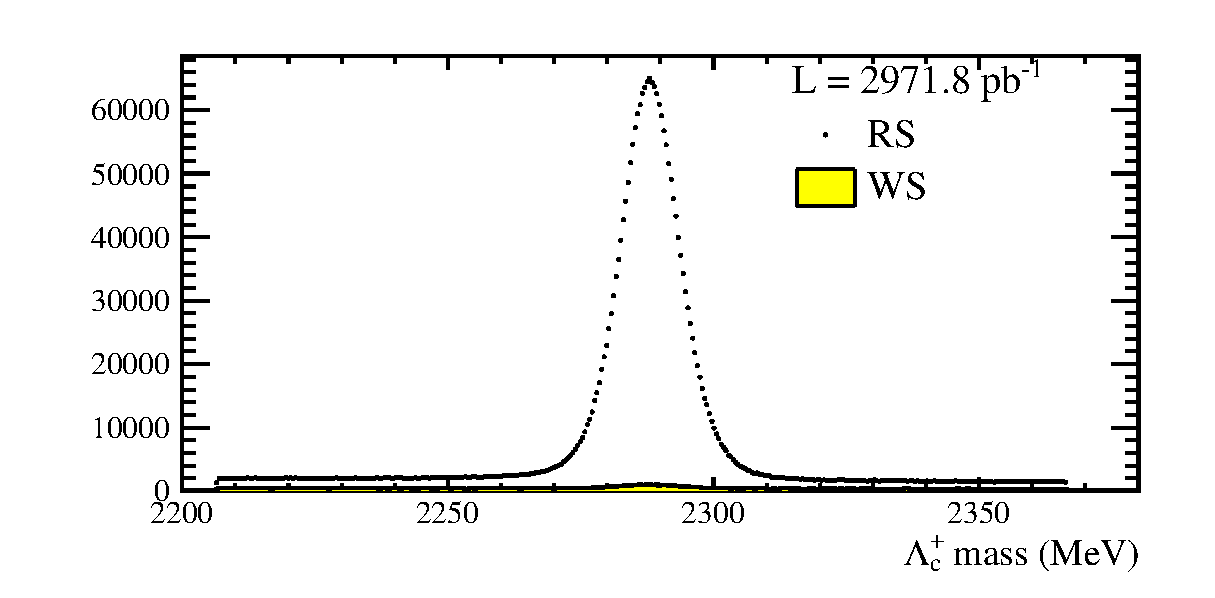
\includegraphics[width=\textwidth]{LbToLc/plots/data/Lc_M}	
	\caption{Plot of the invariant \pKpi mass distribution. A clear mass peak identified as the \Lc can be seen. The yellow shaded area shows events with the WS combination \Lc\mup.}
	\label{fig:plot_Lc_M}
\end{figure}

\subsection{Reconstruction of the \Lb (\Lc\mun) candidate}
The reconstruction of the muon track is completely analogous to the description in Section \ref{sec:Selection_D0mu} and hence not discussed here again.
The combined \Lc\mun, i.e. the \Lb candidate should make a good vertex with a maximum \chisqvtx of 6.
Its DIRA is required to be larger than 0.999.
Being a semileptonic decay again, only a loose selection on the invariant \Lc\mun mass can be applied.
It must have a mass between 2.2 and 8.0 \gev.

Compared to \LbToDpmunuX, main backgrounds are not assumed to be of combinatorial nature, but rather \Lb decays into excited \Lc states.
A good example is the decay \decay{\Lb}{\LcRes{(2595)}\mun\neumb} with \decay{\LcRes{(2595)}}{\Lc\piz}, where the \piz is not reconstructed.
Its decay topology does not differ from \LbToLcmunu, because the \LcRes{(2595)} decays immediately.
However, if the massive \piz is missing in addtion, the the corrected \Lb mass should be shifted to lower masses compared to \LbToLcmunu.
That is why there is not any requirement made on the \Lb corrected mass here.
The different behaviour of the corrected masses is used in the normalisation fit in Chapter \ref{sec:Normalisationfit}  to disentangle the signal from those backgrounds.
\begin{table}[tb]
    \centering
    \caption{Summary of the selection requirements for the reconstruction of \LbToLcmunu candidates.}
    \label{tab:cuts_Lc}
    \begin{tabular}{r|ll}
        \hline
                & Variable          & Value \\
        \hline
        Event   & number of long tracks       & $< 250$ \\
        \hline
        \mun
        & Transverse momentum         & $> 1 \gev$  \\
        & Momentum                    & $> 6 \gev$  \\
        & Ghost probability           & $< 0.5$     \\
        & Track \chisq/ndf            & $< 4$       \\
        & \chisqip w.r.t. PV          & $> 9.0$     \\
        & PIDmu                       & $> 0.3$     \\
        \hline
        \LcTopKpi
        & Daughter momentum           & $> 2 \gev$    \\
        & Daughter transverse momentum& $> 250.0 \mev$\\
        & Daughter ghost probability  & $< 0.5$       \\
        & Daughter \chisqip w.r.t. PV & $> 4.0$       \\
        & \proton daughter PIDp       & $> 10$ \\
        & \proton daughter PIDp$-$PIDK& $> 10$ \\
        & \proton daughter \ptot      & $> 15 \gev$ \\
        & \proton daughter \pt        & $> 1 \gev$ \\
        & \proton daughter \chisqip w.r.t. PV & $> 25 $    \\
        & \Km daughter PIDK           & $> -5.0$     \\
        & \pip daughter PIDK          & $< 20.0$     \\
        & \chisqvtx/ndf               & $< 3$ \\
        & DIRA w.r.t. PV              & $> 0.99$     \\
        & Mass diff. to PDG           & $< 80 \mev$  \\
        & Transverse momentum         & $>2.1 \gev$  \\
        & $\log_{10}$(IP) w.r.t. PV   & $ > - 1.5 $ \\
        & Flight distance \chisq w.r.t. PV  & $> 25$ \\
        \hline
        \Lc\mun
        & Mass                            & $\in \left[2.2, 8.0\right] \gev$ \\
        & \chisqvtx/ndf                   & $< 6$                            \\
        & DIRA w.r.t. PV                  & $> 0.999$                        \\
        \hline
    \end{tabular}
\end{table}

Table \ref{tab:cuts_Lc} summarises all requirements for the reconstruction of the \LbToLcmunu candidates.
After application of all these requirements there are in total 2670999 \LbToLcmunu candidates left for the further analysis. 
Figure \ref{fig:plot_Lb_M_Lc} shows on the left-hand side the invariant mass distribution of the \Lb candidates and on the right-hand side the corrected \Lb mass distribution.
Whereas the \Lb mass is shifted to lower masses due to the missing neutrino, the corrected mass peaks close to the PDG mass of about 5619.5\mev \cite{PDG}.
\begin{figure}[tb]
    \centering
	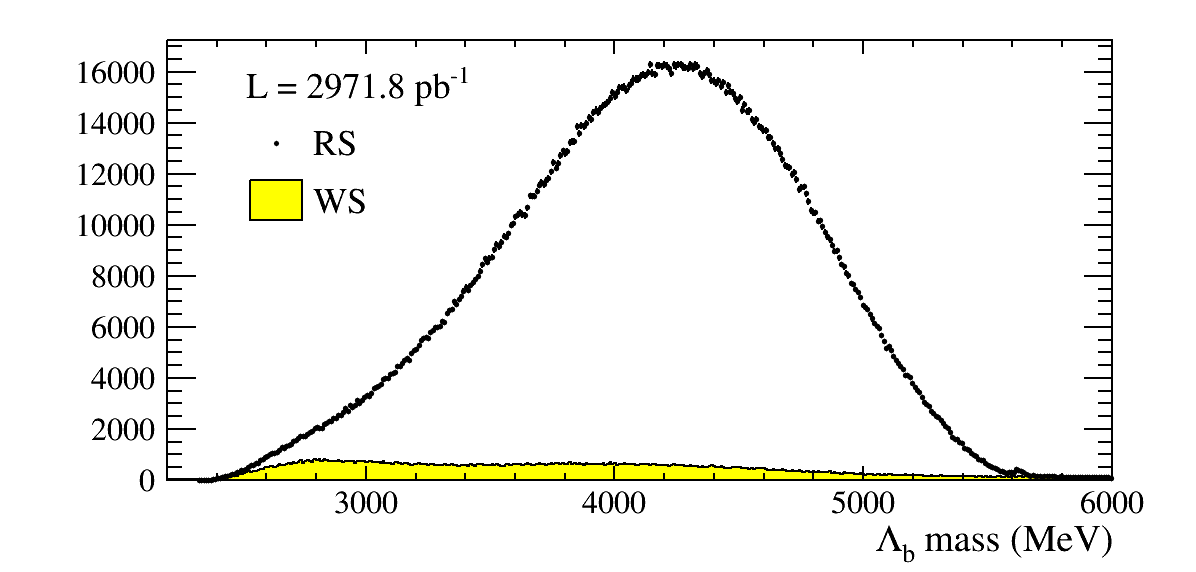
\includegraphics[width=0.49\textwidth]{LbToLc/plots/data/Lb_M} 	
	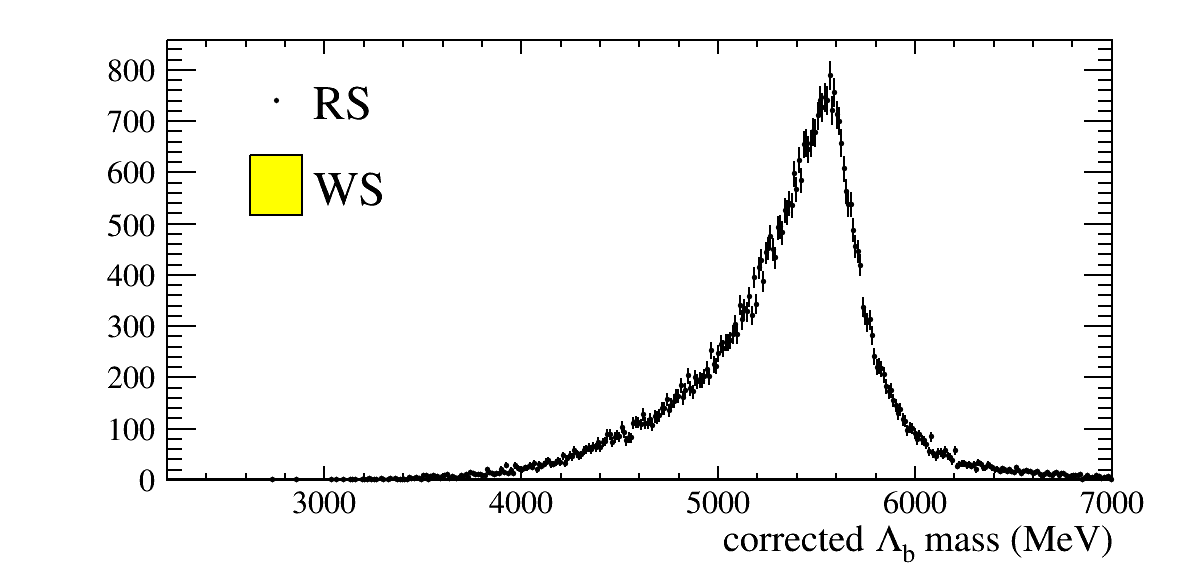
\includegraphics[width=0.49\textwidth]{LbToLc/plots/data/Lb_BPVCORRM}	
	\caption{Plot of the invariant \Lb mass distribution (left) and of the corrected \Lb mass (right). Due to the missing neutrino the \Lb mass peak is shifted to lower masses compared its nominal mass of 5619.5 \mev. With the correction for the missing neutrino, the peak is close to the nominal \Lb
    mass. The yellow shaded area shows events with the WS combination \Lc\mup.}
	\label{fig:plot_Lb_M_Lc}
\end{figure}

	%\chapter{Signal fit}
\label{sec:Signalfit}
This chapter describes the way how the yield \NDp of the signal decays \LbToDpmunuX is determined.
Due to the missing neutrino, the reconstructed \Lb mass does not peak at its actual mass and cannot be used to distinguish signal from background.
Nonetheless the \Dz\proton subsystem is of particular interest.
Recently, \babar measured the decay of two \Lc resonances into \Dz\proton, namely \decay{\LcResI}{\Dz\proton} respectively \decay{\LcResII}{\Dz\proton} \cite{BaBar_D0p}.
It is expected, that the \LcResI and \LcResII also appears in the invariant \Dz\proton mass of the decay \LbToDpmunuX through the decay \decay{\Lb}{\LcRes{(2880/2940)}\mun\neumb} with \decay{\LcRes{(2880/2940)}}{\Dz\proton}.
Indeed, there are some peaking structures at \MDp around 2880\mev and 2940\mev as Figure \ref{fig:plot_mD0p_logIP} (top) shows.
As a nice side effect, the masses and widths of those resonances can be determined, too.
However, it is expected that most of the \LbToDpmunuX decays are nonresonant, i.e. they decay directly into the $\Dz\proton\mun\neumb X$ final state without going through an intermediate resonance.
It should be stressed, that the measurement of \BR(\LbToDpmunuX) is an inclusive measurement.
This means, that every decay of a \Lb into a final state including a \Dz\proton\mun\neumb is considered as signal.
Thus, the nonresonant \Lb decays as well as the decays via the \LcResI and \LcResII resonances are counted to the signal yield \NDp.

Unfortunately, the nonresonant \Lb decays cannot be disentangled in the \Dz\proton mass from combinatorial background like \BToDmunuX with randomly combined protons.
As already mentioned in Section \ref{sec:Backgrounds}, an appropriate discriminating variable between signal and those combinatorial backgrounds is \logIP.
Just to remind, it has been defined as the logarithm of the difference between the \chisqvtx of the \Dz\mun candidate with and without the proton, i.e. $\logIP := \log\left[\chisqvtx(\Dz\proton\mun) - \chisqvtx(\Dz\mun)\right]$.
The smaller \logIP, the better the proton makes a vertex with the \Dz\mun candidate and the more likely it is a \LbToDpmunuX signal event.
Figure \ref{fig:plot_mD0p_logIP} (bottom) illustrates the discriminating power of \logIP when one compares the data and the wrong sign distributions.

The strategy for the signal fit is to perform a two-dimensional binned likelihood fit to the \Dz\proton mass to learn as much about intermediate resonant states as possible and simultaneously to the \logIP distribution to disentangle \LbToDpmunuX signal from combinatorial background.
Unfortunately, there is no theoretical description of the \LbToDpmunuX decay and the distributions of \MDp and \logIP.
Thus, the most important task is to find a proper parametrisation of the two-dimensional distribution on an empirical basis.
Depending on the respective variables either data driven methods or simulations are used for that purpose as will be described in the following section.

% ==================================
% Section: Fit parametrisation
% ==================================
\section{Empiric determination of the shape of the two-dimensional \logIP/\MDp distribution}
This section describes the determination of the shapes for the \logIP distribution and the \Dz\proton mass shape.
Though there will be a two-dimensional fit in the end, it is assumed that the \logIP and \MDp distributions can be determined separately for each fit component.
The two-dimensional fit is rather needed for the separation of the different fit components, for instance the \MDp shapes are very similar for nonresonant signal and background but completely differ in their \logIP shape, i.e. their vertex quality.

For \logIP, the functions to be fitted on data are determined with simulations.
This determination is done for signal and background separately.
Both shapes are then combined and fitted to data.

Concerning the invariant \Dz\proton mass, there do not exist any reliable simulations predicting its shape.
Here it is assumed that the behaviour of the combinatorial background component is similar to the wrong sign events.
Hence, the \MDp distribution of the wrong sign events is used to get the shape of the background component.
The signal component is determined with the data itself.
To highly suppress combinatorial background leaking into the \Dz\proton mass distribution, only events with a $\logIP < 1$ are fitted.
This corresponds to the distribution shown in Figure \ref{fig:plot_mD0p_logIP} (top).

\subsection{\logIP shape}
As already mentioned both, \logIP signal and background components, are determined with simulations.
The \logIP distribution of the signal simulation in Figure \ref{fig:fit_logIP_signal} reminds of a Gaussian curve, but having different widths to the left and the right from the maximum.
Thus, it is parametrised with a so called \textsc{bifurcated Gaussian}.
A bifurcated Gaussian is an asymmetric Gaussian with two different widths for the left and the right part from the maximum.
If $\mathcal{G}(x|x_0,\sigma) = \frac{1}{\sqrt{2\pi}\sigma}\exp\left(-\frac{x-x_0}{2\sigma}\right)$ denotes a usual Gaussian with mean $x_0$ and width $\sigma$, a Bifurcated Gaussian can be written as\footnote{All fitfunctions in the following are given without normalisation factors. That is why there always appears a $\propto$ sign instead of an equal sign.}
\begin{align}
    \text{BfG}(x|x_0, \sigma_{\text{L}}, \sigma_{\text{R}}) \propto 
    \begin{cases}
        \mathcal{G}(x|x_0,\sigma_{\text{L}}) & \text{for } x < x_0 \\   
        \mathcal{G}(x|x_0,\sigma_{\text{R}}) & \text{for } x > x_0 \\   
    \end{cases},
\end{align}
The tails on both sides of \logIP are very broad compared to the peaking part.
Thus a single bifurcated Gaussian is not sufficient.
The final fit function for the signal \logIP shape is the sum of two bifurcated Gaussians, in the following called a double Bifurcated Gaussian DBfG
\begin{align}
    &\text{DBfG}(x|x_0,\vec{\sigmaL{}}, \vec{\sigmaR{}}, f_{\BfG_1}) \propto \nonumber \\
    &f_{\BfG_1} \BfG(x|x_0,\sigmaL{1}, \sigmaR{1}) + \left(1 - f_{\BfG_1} \right) \BfG(x|x_0,\sigmaL{2}, \sigmaR{2}),
\end{align}
where $f_{\BfG_1}$ denotes the fraction of the first \BfG and the two \BfG share a common mean $x_0$. 
The fit result for the signal simulation can be seen in Figure \ref{fig:fit_logIP_signal}.
\begin{figure}[ptb]
    \centering
	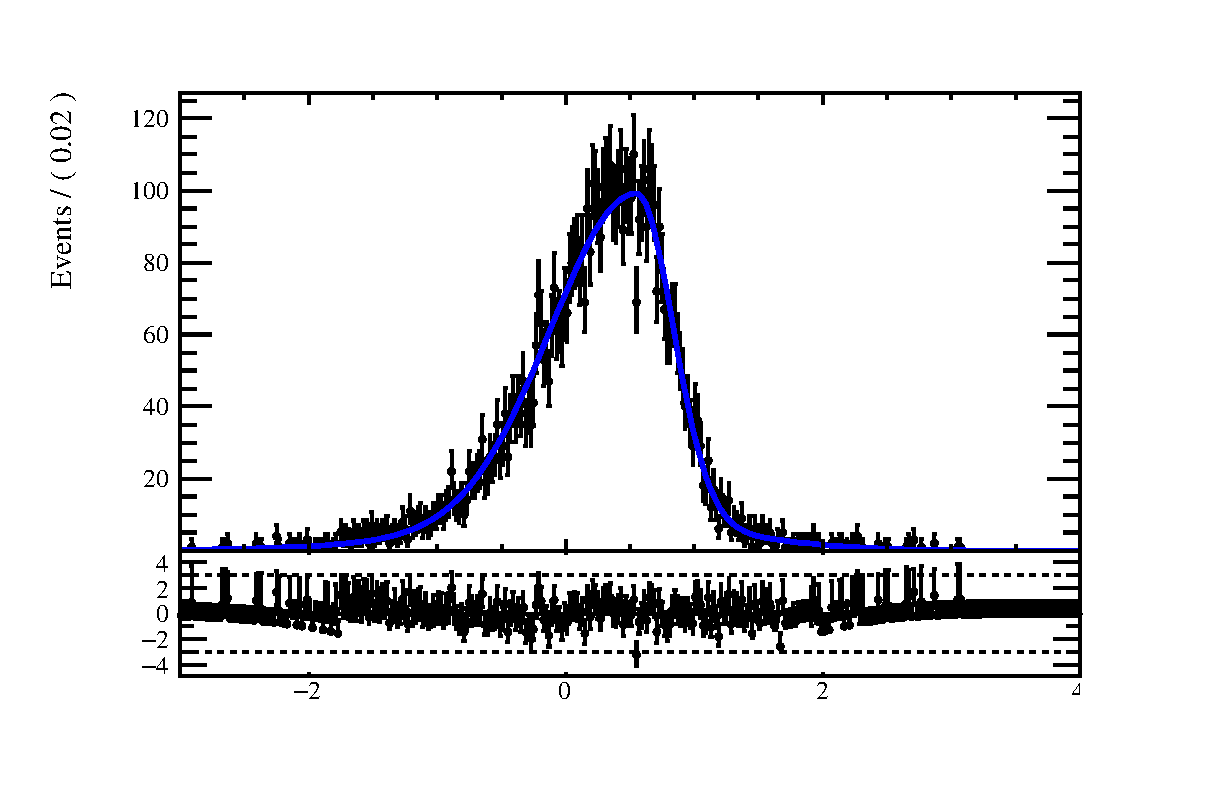
\includegraphics[width=0.75\textwidth]{LbToD0p/fits/MC_D0p_SIG/logIP_RS/fit_DBfG}
	\caption{Fit to the \logIP distribution of the signal simulation. As parametrisation a double Bifurcated Gaussian has been chosen.}
    \label{fig:fit_logIP_signal}
\end{figure}
In order to estimate the quality of the fit, the \textsc{pull} distribution is also shown in Figure \ref{fig:fit_logIP_signal} below the \logIP distribution.
The pull of a variable $x$ is defined as
\begin{align}
    \text{pull}(x) = \frac{N_\text{meas}(x)-N_\text{fit}(x)}{\sigma_{N_\text{meas}}(x)}.  \label{eq:pull}
\end{align}
Referring to Figure \ref{fig:fit_logIP_signal}, $N_\text{meas}(x)$ denotes the number of entries in the bin with $\logIP = x$, $N_\text{fit}(x)$ the corresponding result of the fit in the respective bin and $\sigma_{N_\text{meas}}(x)$ the error on $N_\text{meas}(x)$.
In other words, the pulls are the residuals of the fit normalised to the uncertainty.
If the fit describes the data well, the pull distribution should peak and fluctuate around zero with mean 1 \cite{Pulls}.
From the pull distribution it can be stated that the chosen fit model describes the data well, especially in the tails.
A little bias might be included if on closer looks at the region of $\logIP \approx 0$.

Concerning the \logIP background shape, only a simulation with very little statistics is available.
To get a better idea of the background \logIP shape and to increase statistics, right sign and wrong sign events of this sample have been added.
In this case wrong sign events refers to events with a \Lc\mup in the final state.
Compared to the signal \logIP shape, both, right sign and wrong sign events, describe combinatorial background.
Thus, it is assumed that their \logIP shapes are similar as Figure \ref{fig:plot_logIP_MC_BKG} confirms. 
According to this, the addition of right sign and wrong sign is appropriate to increase statistics in this case.

The \logIP distribution of the background simulation looks lika a Gaussian around the maximum, but has a long tail to lower \logIP values.
That is why a single CrystalBall function is chosen as fit function for the \logIP background shape. 
This function was first used by the CrystalBall collaboration to account for radiative losses in \jpsi or \psitwos decays \cite{CrystalBall}. 
It is defined as 
\begin{align}
    &\CB(x|x_0, \sigma, \alpha, n) \propto
    \begin{cases}
        \exp \left(-\frac{(x-x_0)^2}{2\sigma^2}\right)     & \text{for } \frac{x-x_0}{\sigma} > -\alpha \\
        A \cdot \left(B - \frac{x-x_0}{\sigma}\right)^{-n} & \text{for } \frac{x-x_0}{\sigma} \leq -\alpha
    \end{cases}, \\
    &\text{where} \nonumber\\
    &A = \left(\frac{n}{|\alpha|}\right)^n \exp\left(-\frac{|\alpha|^2}{2}\right), \\
    &B = \frac{n}{|\alpha|} - |\alpha|.
\end{align}
Hence, the CrystalBall function is a Gaussian with an enhanced tail at one side of the maximum, due to the power law for $\frac{x-x_0}{\sigma} \leq -\alpha$.
So $\alpha$ denotes the transition between the Gaussian and the power law tail and $n$ the latter's exponent.

The result of the fit to the background simulation can be seen in Figure \ref{fig:fit_logIP_MC_BKG}.
According to the pull distribution the fit nicely describes the data points.
Nonetheless one has to note that statistics here are very little.
\begin{figure}[ptb]
    \centering
	\includegraphics[width=0.75\textwidth]{LbToD0p/plots/MC_B2D0munu_BKG/logIP}
	\caption{Comparison of the \logIP distribution for right sign and wrong sign events in the background simulation. Both, the shapes for right sign and wrong sign are very similar and thus can be added to increase statistics.}
    \label{fig:plot_logIP_MC_BKG}
\end{figure}
\begin{figure}[ptb]
    \centering
	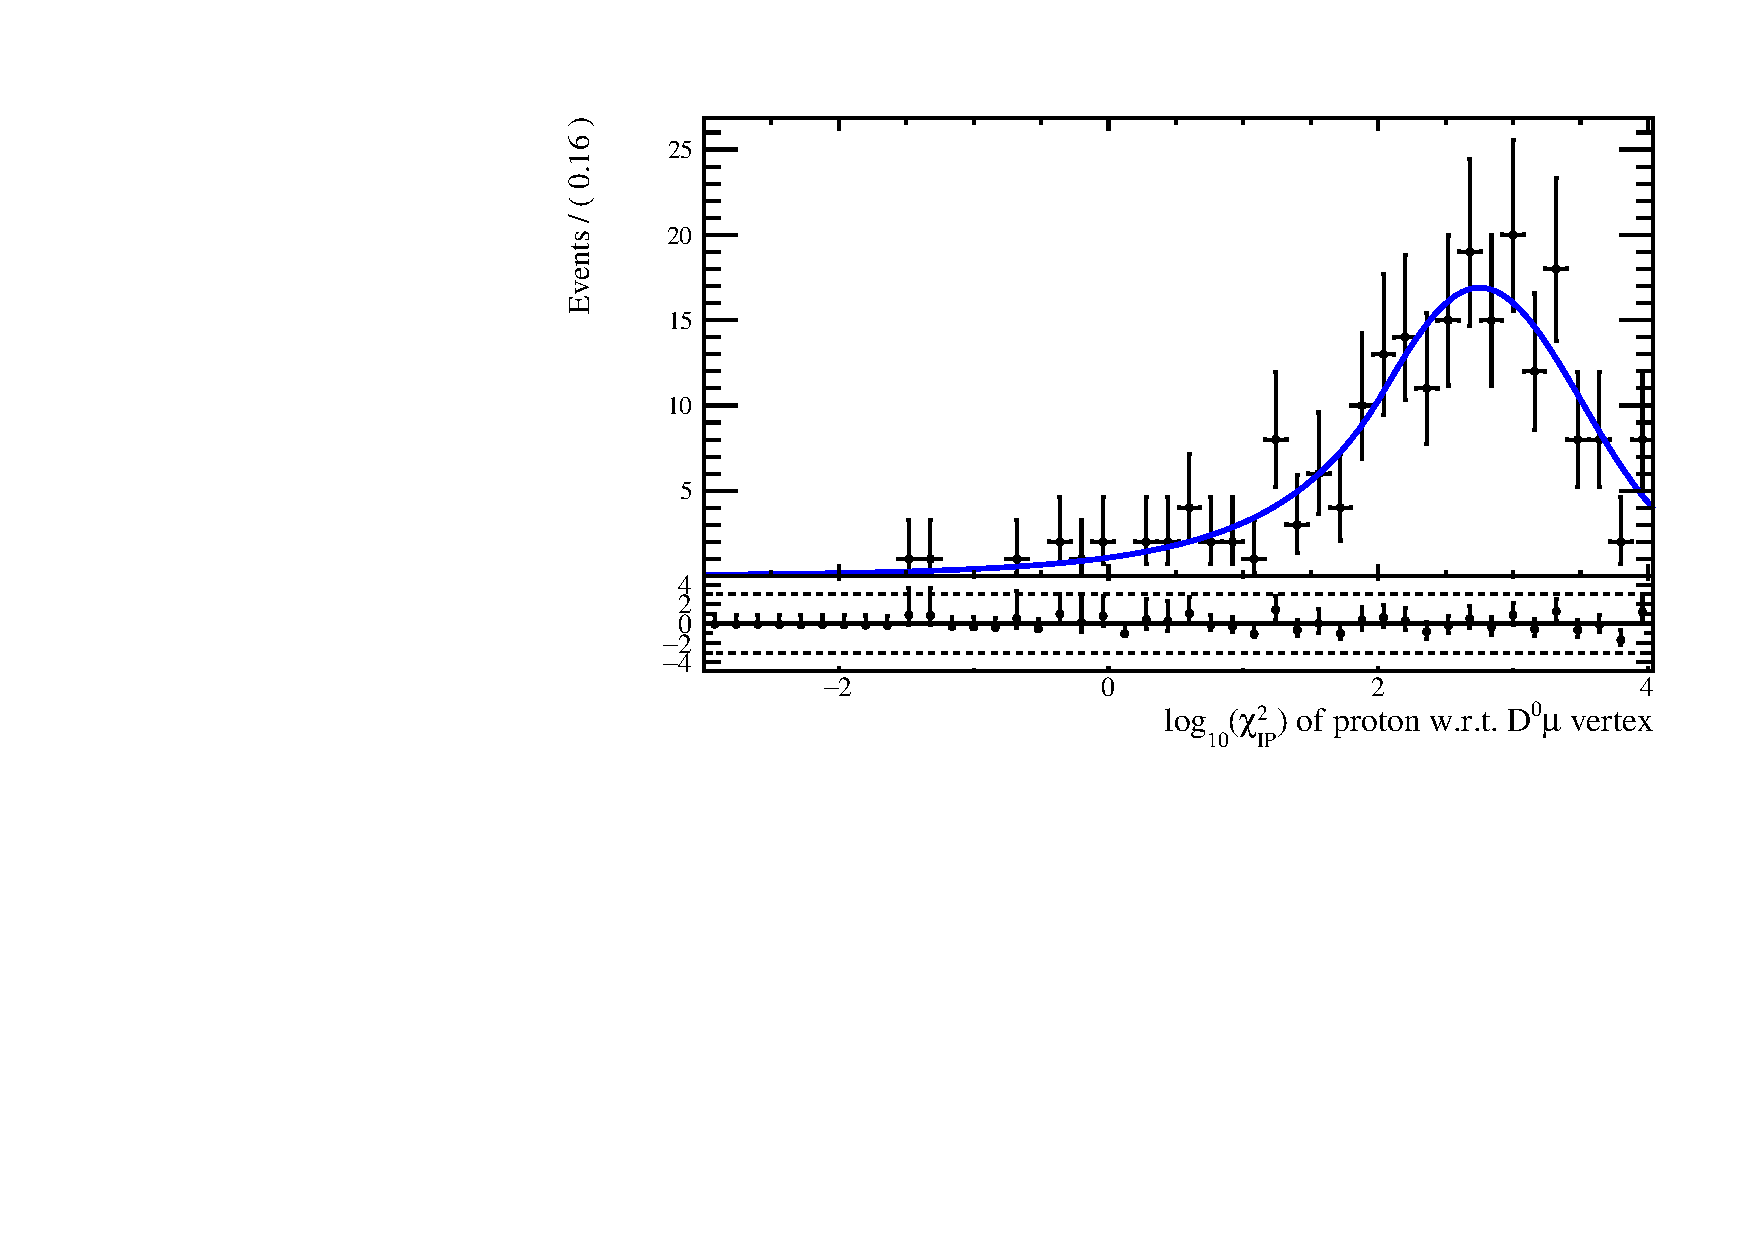
\includegraphics[width=0.75\textwidth]{LbToD0p/fits/MC_B2D0munu_BKG/logIP_RS/fit_CB}
	\caption{Fit to the (RS and WS added) \logIP shape of the background simulation.
             The distribution is modeled with a CrystalBall function.}
    \label{fig:fit_logIP_MC_BKG}
\end{figure}

\subsection{One-dimensional fit to the \logIP distribution in data}
\label{sec:ControlLogIP}
To control if the chosen parametrization of the \logIP distribution gained from simulation describes data, a one-dimensional \logIP-fit on data is performed.
For that purpose, the double bifurcated Gaussian as signal component and the CrystalBall as background component are added, i.e. the total probabiltiy density function $\mathcal{P}$ for that fit is:
\begin{align}
    &\mathcal{P}(x|N_\text{sig}, N_\text{bkg}, x_{0, \text{sig}}, x_{0, \text{bkg}} \vec{\sigmaL{}}_{,\text{sig}}, \vec{\sigmaR{}}_{,\text{sig}}, f_{\BfG_1}, \sigma_\text{bkg}, \alpha, n) \propto \nonumber\\
    &N_\text{sig} \DBfG(x|x_{0, \text{sig}}, \vec{\sigmaL{}}_{,\text{sig}}, \vec{\sigmaR{}}_{,\text{sig}}, f_{\BfG_1}) + N_\text{bkg} \CB(x| x_{0, \text{bkg}}, \sigma_\text{bkg}, \alpha, n)
\end{align},
where $N_\text{sig}$ denotes the signal yield and $N_\text{bkg}$ the background yield respectively.
The fitresult can be seen in Figure \ref{fig:fit_logIP_RS} and the corresponding yields and parameter values are listed in Table \ref{tab:logIP_RS}.
\begin{figure}[ptb]
    \centering
	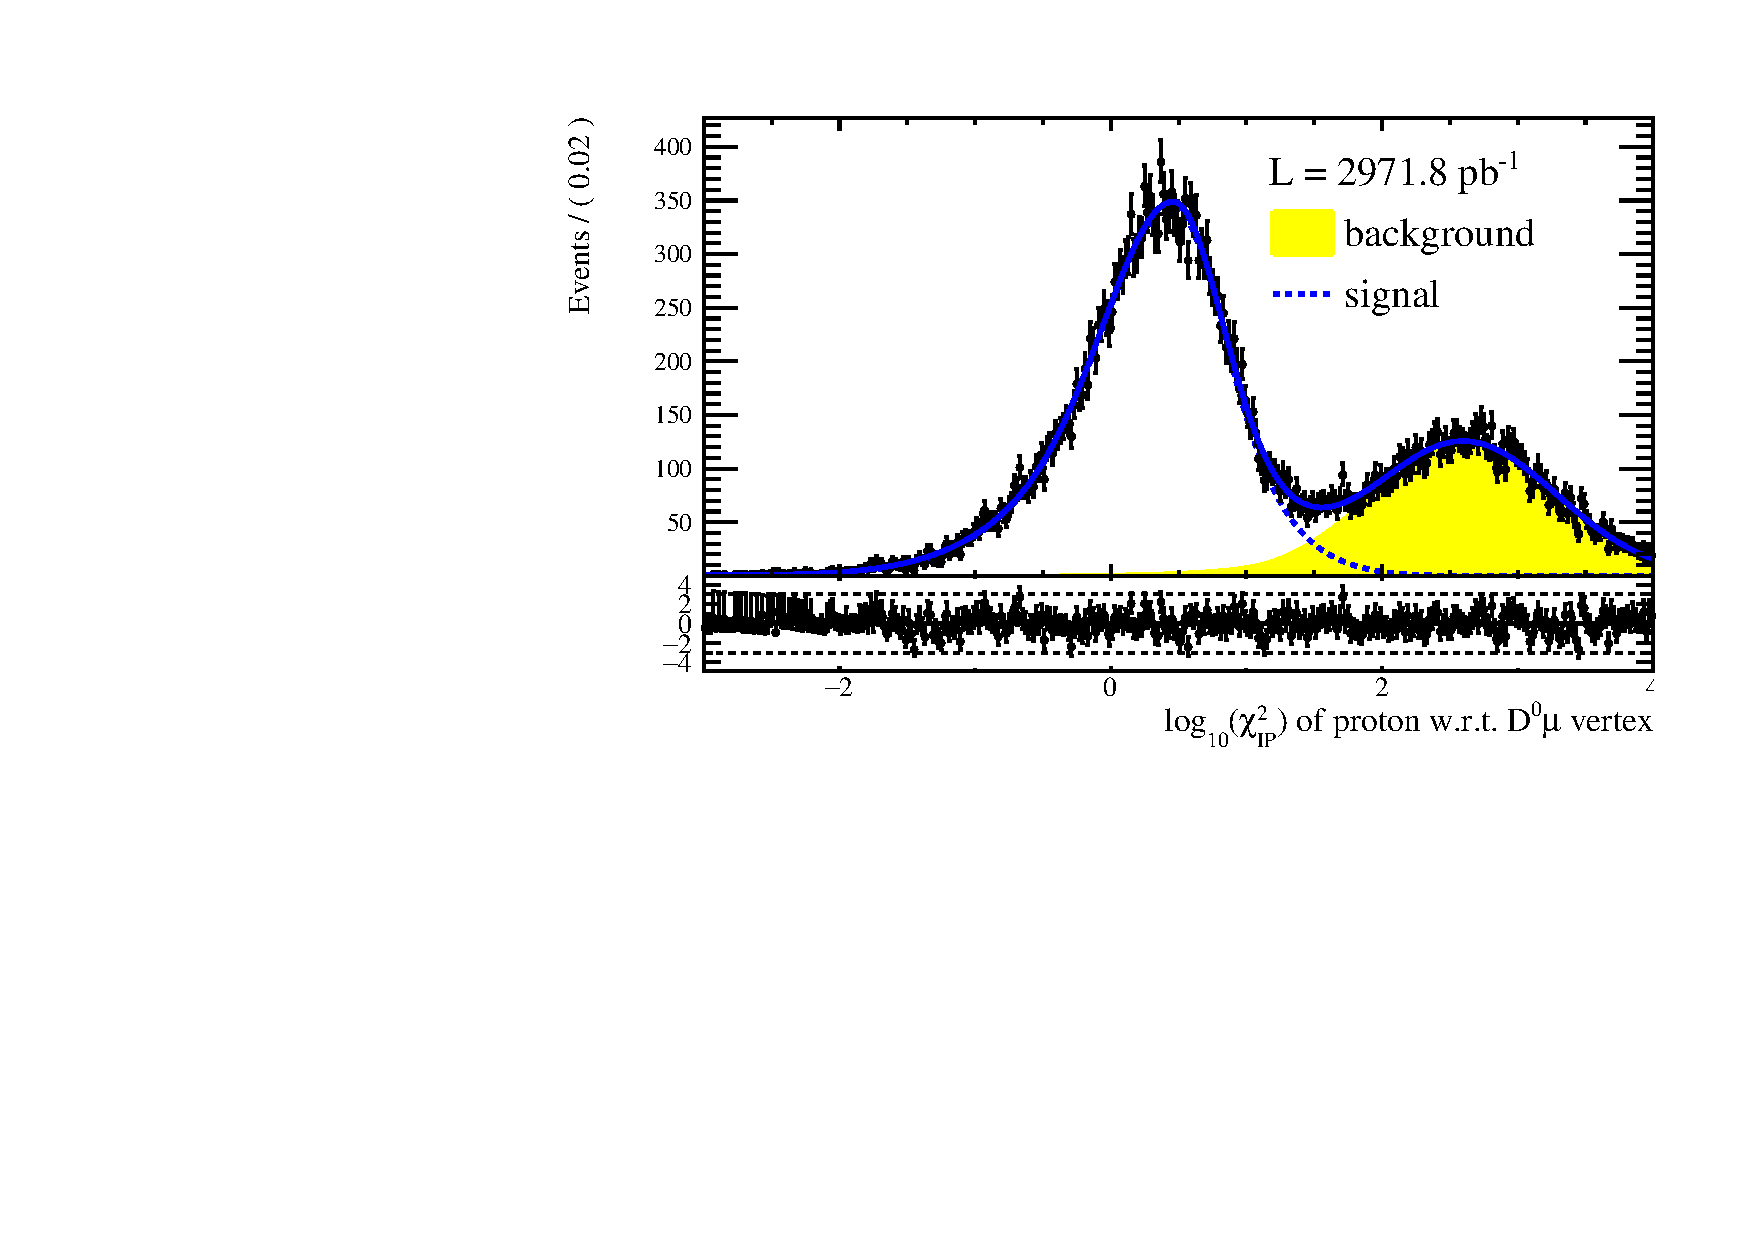
\includegraphics[width=\textwidth]{LbToD0p/fits/data/logIP_RS/fit_DBfG_CB}
	\caption{\logIP distribution of the data sample.
             A binned likelihood fit is performed on it with the sum of a double bifurcated Gaussian for the signal (blue, dashed line) and a CrystalBall function for the background component (yellow shaded). }
    \label{fig:fit_logIP_RS}
\end{figure}
 
\begin{table}[h]
    \centering
    \caption{Results of the onedimensional \logIP fit on data.}
    \label{tab:logIP_RS}
    $\begin{array}{lr@{\pm}l}
    \hline
    \text{Variable} & \multicolumn{2}{c}{\text{Value}} \\
    \hline
        \multicolumn{3}{l}{\text{\textbf{Yields}}} \\
\text{signal yield}&(2.325 & 0.028) \cdot 10^{4}\\
\text{background yield}&(1.086 & 0.026) \cdot 10^{4}\\
\multicolumn{3}{l}{\text{\textbf{Signal (\DBfG)}}} \\
\text{mean}&(4.59 & 0.26) \cdot 10^{-1}\\
\text{left width 1}&(8.72 & 0.56) \cdot 10^{-1}\\
\text{right width 1}&(5.74 & 0.44) \cdot 10^{-1}\\
\text{left width 2}&(4.72 & 0.55) \cdot 10^{-1}\\
\text{right width 2}&(3.37 & 0.23) \cdot 10^{-1}\\
\text{fraction BfG 1}&(5.61 & 0.89) \cdot 10^{-1}\\
\multicolumn{3}{l}{\text{\textbf{Background (\CB)}}} \\
\text{CB mean}&(2.6 & 0.017) \cdot 10^{0}\\
\text{CB $\sigma$}&(6.85 & 0.14) \cdot 10^{-1}\\
\text{CB $\alpha$}&(2.035 & 0.099) \cdot 10^{0}\\
\text{CB $n$}&(1.62 & 0.45) \cdot 10^{0}\\

\hline
\end{array}$
\end{table}
    

The chosen model very nicely describes the data as can be seen in the pull distribution.
Thus the chosen parametrisation for the \logIP shape is reasonable.
This fit is later also used for systematic studies, since it is already able to distinguish between signal and background yields, see Chapter \ref{sec:Selection} for further discussions.

\subsection{\Dz\proton mass shape}
\label{sec:Shape_mD0p}
To get an idea of the (combinatorial) background shape in the \Dz\proton mass distribution, events with a wrong sign proton, i.e. events with \Dz\antiproton\mun in the final state are used since the transition from \Lb to a \Dz\antiproton\mun final state is physically forbidden by charge
conservation and should thus give a good proxy for randomly combined \LbToDpmunu candidates. 
The \MDp distribution of these wrong sign events is shown in Figure \ref{fig:fit_mD0p_WS} and modeled with an empirical background function
\begin{align}
    \text{EBG}(m|m_0, m_1, m_2, p,c_1) = \text{PS}(m|m_1,m_2) \cdot (m - m_0)^p \cdot \exp\left[ c_1 \left(1-\frac{m_0}{m}\right)\right], \label{eq:EBG}
\end{align}
where $m_0 := m_1 + m_2$ denotes the kinematic \Dz\proton mass threshold and PS the phase space function
\begin{align}
    \text{PS}(m|m_1,m_2) = \frac{1}{2m} \sqrt{\left[m^2 - (m_1 + m_2)^2\right] \left[m^2 - (m_1 - m_2)^2\right]}. \label{eq:PS}
\end{align}
Here and in the following fits, $m_1$ and $m_2$ are fixed to the \Dz respectively proton PDG mass values.
Figure \ref{fig:fit_mD0p_WS} shows the result of the fit.
Again, the model nicely describes the distribution.
It should be noted here, that there is no structure observed in this wrong sign mass spectrum.
This is a good confirmation, that the identification of the two peaks in the \Dz\proton mass for right sign events as \LcResI and \LcResII is appropiate.
\begin{figure}[ptb]
    \centering
	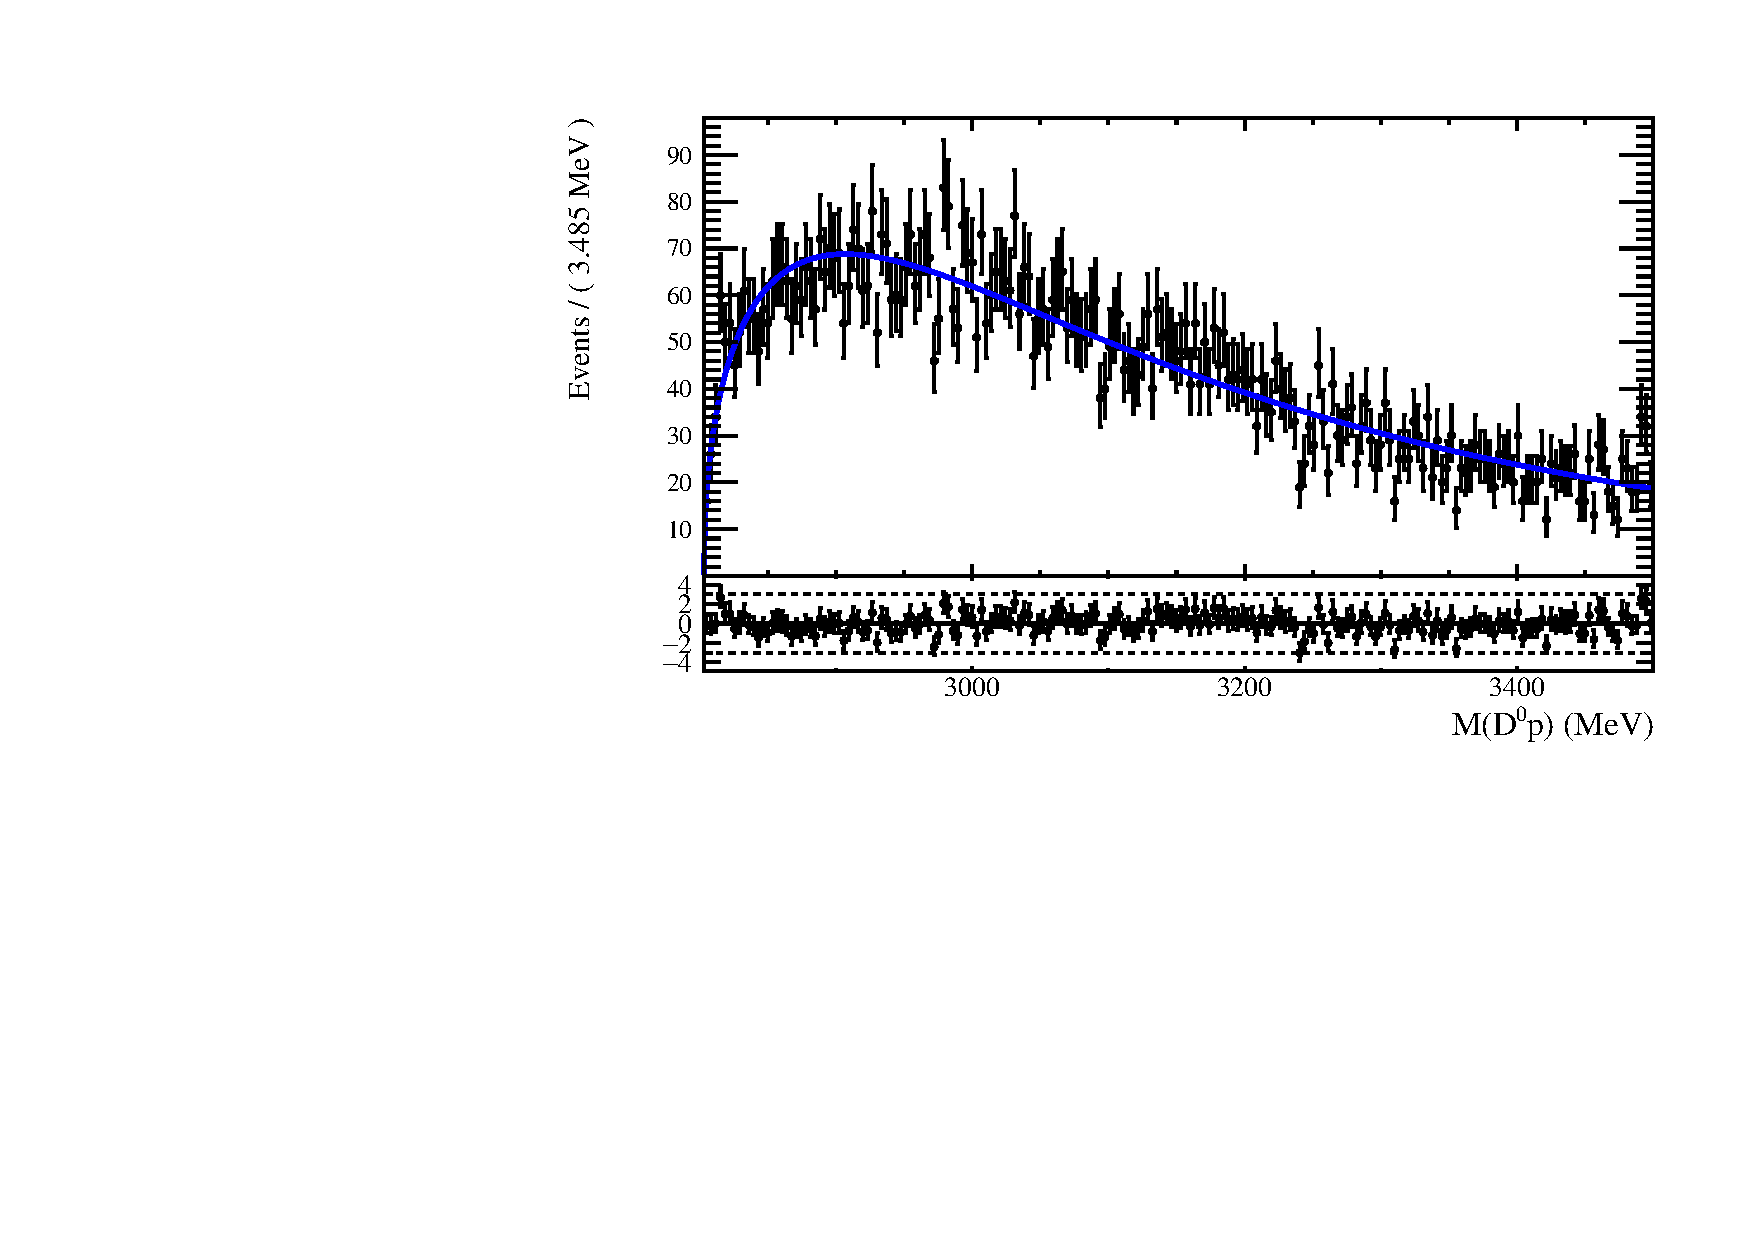
\includegraphics[width=0.75\textwidth]{LbToD0p/fits/data/mD0p_WSp/fit_EmpiricBG}
	\caption{Fit to \Dz\proton mass of wrong sign proton events.
             As model an empiric background function has been chosen, see equation (\ref{eq:EBG})}
    \label{fig:fit_mD0p_WS}
\end{figure}

Unfortunately, there is no reliable simulation predicting the mass shape for the \Dz\proton invariant mass. 
A shape for the signal therefore has to be determined empirically on data. 
A fit to the \Dz\proton mass distribution is applied with the requirement that the \Dz\proton\muon system makes a good vertex, i.e. $\logIP < 1$.
It is shown in Figure \ref{fig:fit_mD0p_RS} top.
This hard requirement strongly suppresses combinatorial background and allows to determine the signal distribution.
As already stated before, the main part of the signal will be nonresonant.
Besides that it is expected to see the two \LcResI and \LcResII resonances.
They are parametrised by a relativistic Breit-Wigner distribution convoluted with a double Gaussian to account for the detector's mass resolution.
The relativistic Breit-Wigner distribution is defined as follows:
\begin{align}
    \text{RelBW}(m|m_R, m_1, m_2, \Gamma_0) \propto 
    \frac{m \Gamma(m|m_R, m_1, m_2, \Gamma_0)}{(m^2-m_R^2)^2 + (m_R \Gamma(m|m_R, m_1, m_2, \Gamma_0))^2}, \label{eq:RelBW}
\end{align}
with 
\begin{align}
    \Gamma(m|m_R, m_1, m_2, \Gamma_0) = \Gamma_0 \frac{m_R}{m} \frac{\PS(m| m_1, m_2)}{\PS(m_R| m_1, m_2)}, 
\end{align}
where PS denotes the phase space function of equation (\ref{eq:PS}), $m_R$ the resonance's mass and $\Gamma_0$ its width \cite{Lb_FF}.
Thus, each resonance is modeled with
\begin{align}
    &\text{RES}(m| m_R, m_1, m_2, \Gamma_0, \sigma_1, \sigma_2, f_1) \propto \nonumber \\
    &\text{RelBW}(m| m_R, m_1, m_2, \Gamma_0) \otimes \left[f_1 \mathcal{G}(m|0,\sigma_1) + (1-f_1) \mathcal{G}(m|0,\sigma_2) \right] \label{eq:RES}
\end{align}
The determination of the mass resolution is thoroughly described in section \ref{sec:Massresolution}. 
The obtained resolution will be fixed in all fits later.

The non-resonant signal part is modeled with the sum of two exponential functions multiplied by a turn-on function.
\begin{align}
    \text{TDExp}(m|m_0, c_0, c_1, c_2, f_{c_1}) \propto \left( 1 - \mathrm{e}^{c_0(m-m_0)} \right) \cdot \left[ f_{c_1} \mathrm{e}^{c_1m} + (1-f_{c_1}) \mathrm{e}^{c_2m} \right]. \label{eq:TDExp}
\end{align}
The turn-on factor is needed to model the steep rise at the \Dz\proton mass threshold.

The fit to the invariant \Dz\proton mass distribution that is shown on the upper side of Figure \ref{fig:fit_mD0p_RS} does not describe the data at low \Dz\proton mass.
Different models for the non-resonant component have been tried to describe this steep curvature without success.
However, when adding another resonant component, the fit converges and describes the data well as can be seen on the lower side of Figure \ref{fig:fit_mD0p_RS}.
This additional component will be labeled ``low mass enhancement" throughout the analysis.
Thus, the total fit function consists of four parts: 
The non-resonant part modeled with the ``turn-on double exponential" function TDExp of eq. (\ref{eq:TDExp}) and relativistic Breit-Wigner functions according eq. (\ref{eq:RES}) for the \LcResI, \LcResII and the low mass enhancement. 
The fit results can be seen in Figure \ref{fig:fit_mD0p_RS} (right) and Table \ref{tab:fit_mD0p_RS}.

Note that at this point, the additional resonant component, the low mass enhancement, is merely introduced to enable the fit to converge and match the data.
There are several possible reasons for such an enhancement.
Nonetheless there is some motivation to choose a resonant model as additional component:
On the one hand the peak looks similar to the other resonances.
On the other hand, there is a similar peak seen in other analyses e.g. \babar is discussing a (much less pronounced) peak at an invariant \Dz\proton mass of about 2840\mev in its study on the \Dz\proton final state in \cite{BaBar_D0p}.
The reason for this peak is not understood so far and is currently studied in different ongoing \lhcb analyses.
Besides some detector effects, backgrounds or kinematical reflections it is not excluded that a new particle is seen here.
A thorough discussion, if this additional component is actually needed and what might cause this peak follows in section \ref{sec:Structure}.
In the following this component is treated as signal since it appears very clear when requiring $\logIP < 1$, i.e. in the background suppressed region making a good decay vertex.
\begin{figure}[ptb]
    \centering
	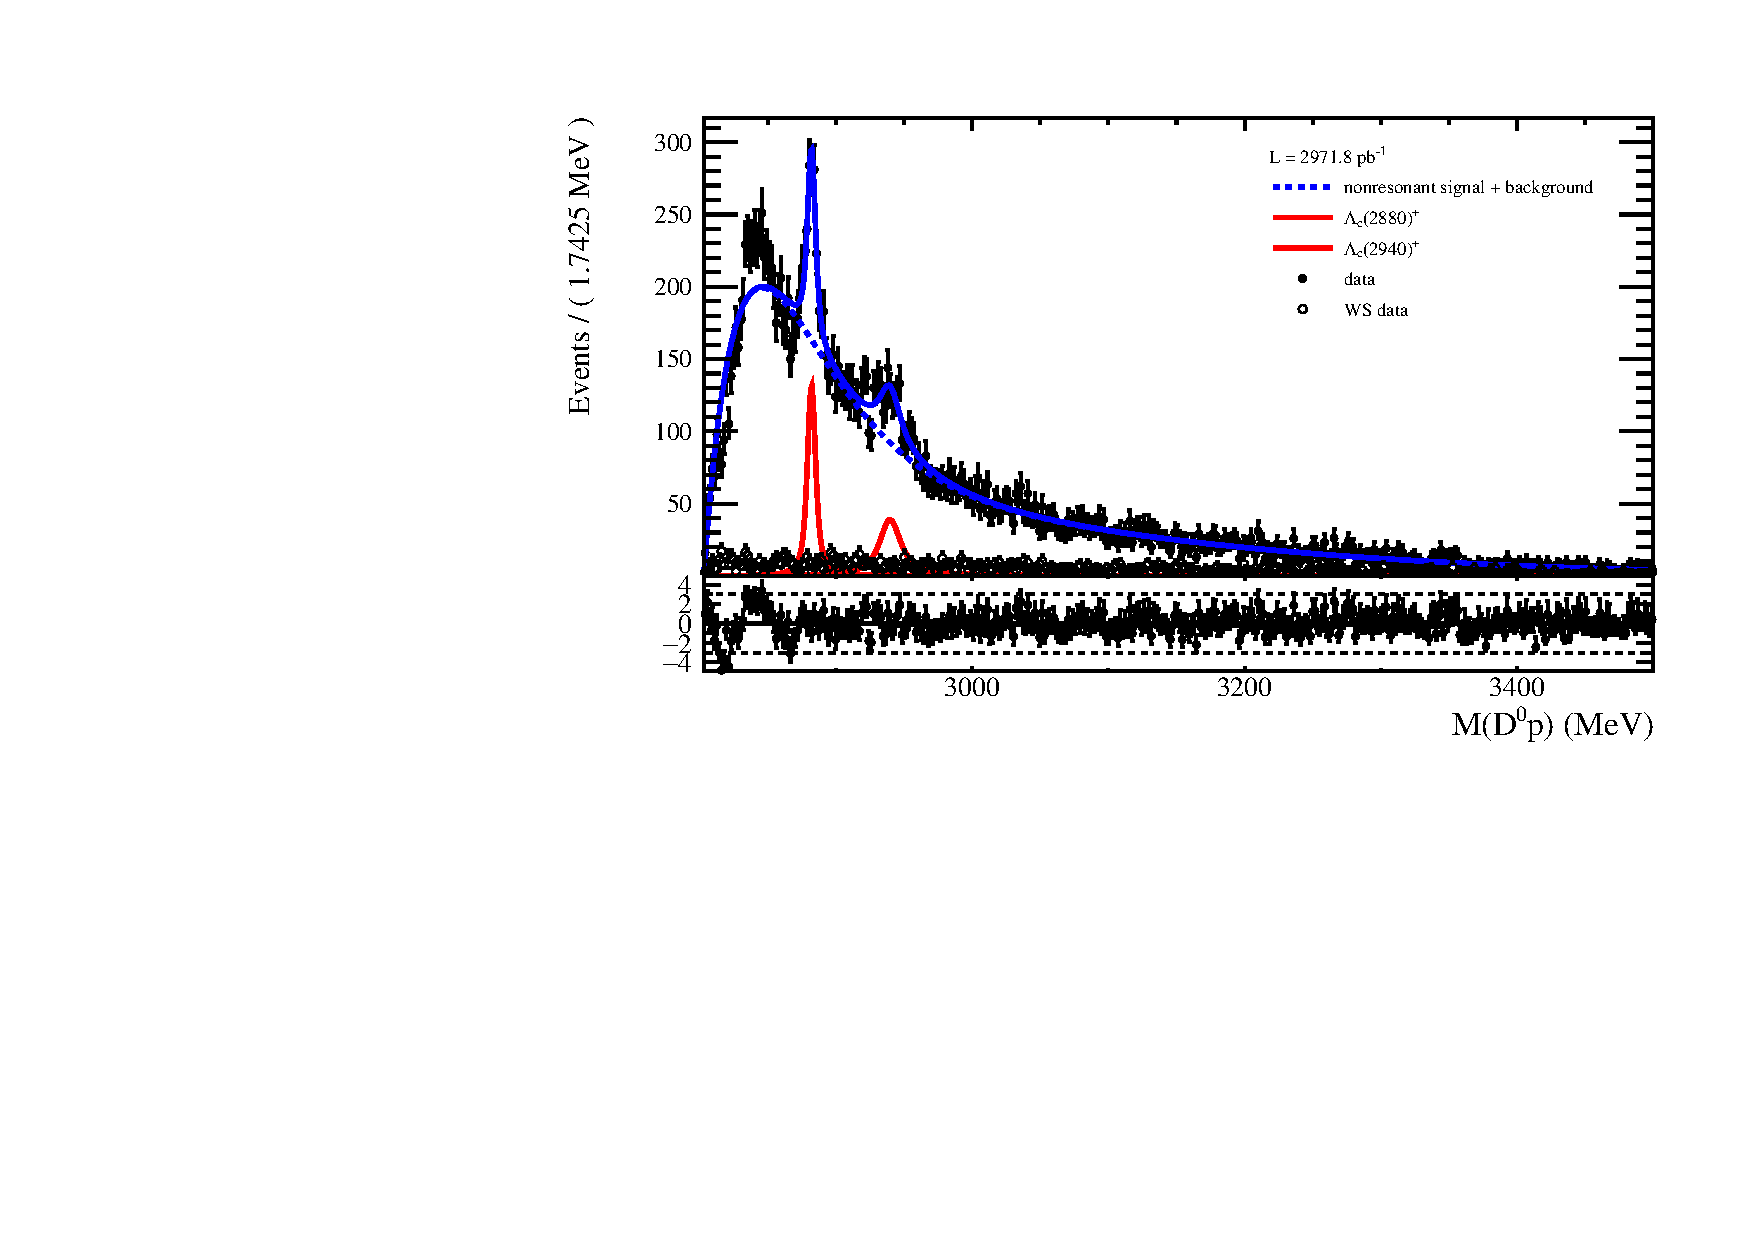
\includegraphics[width=\textwidth]{LbToD0p/fits/data/mD0p_RS/fit_TurnOnDExp_2RelBWPSRes} \\
	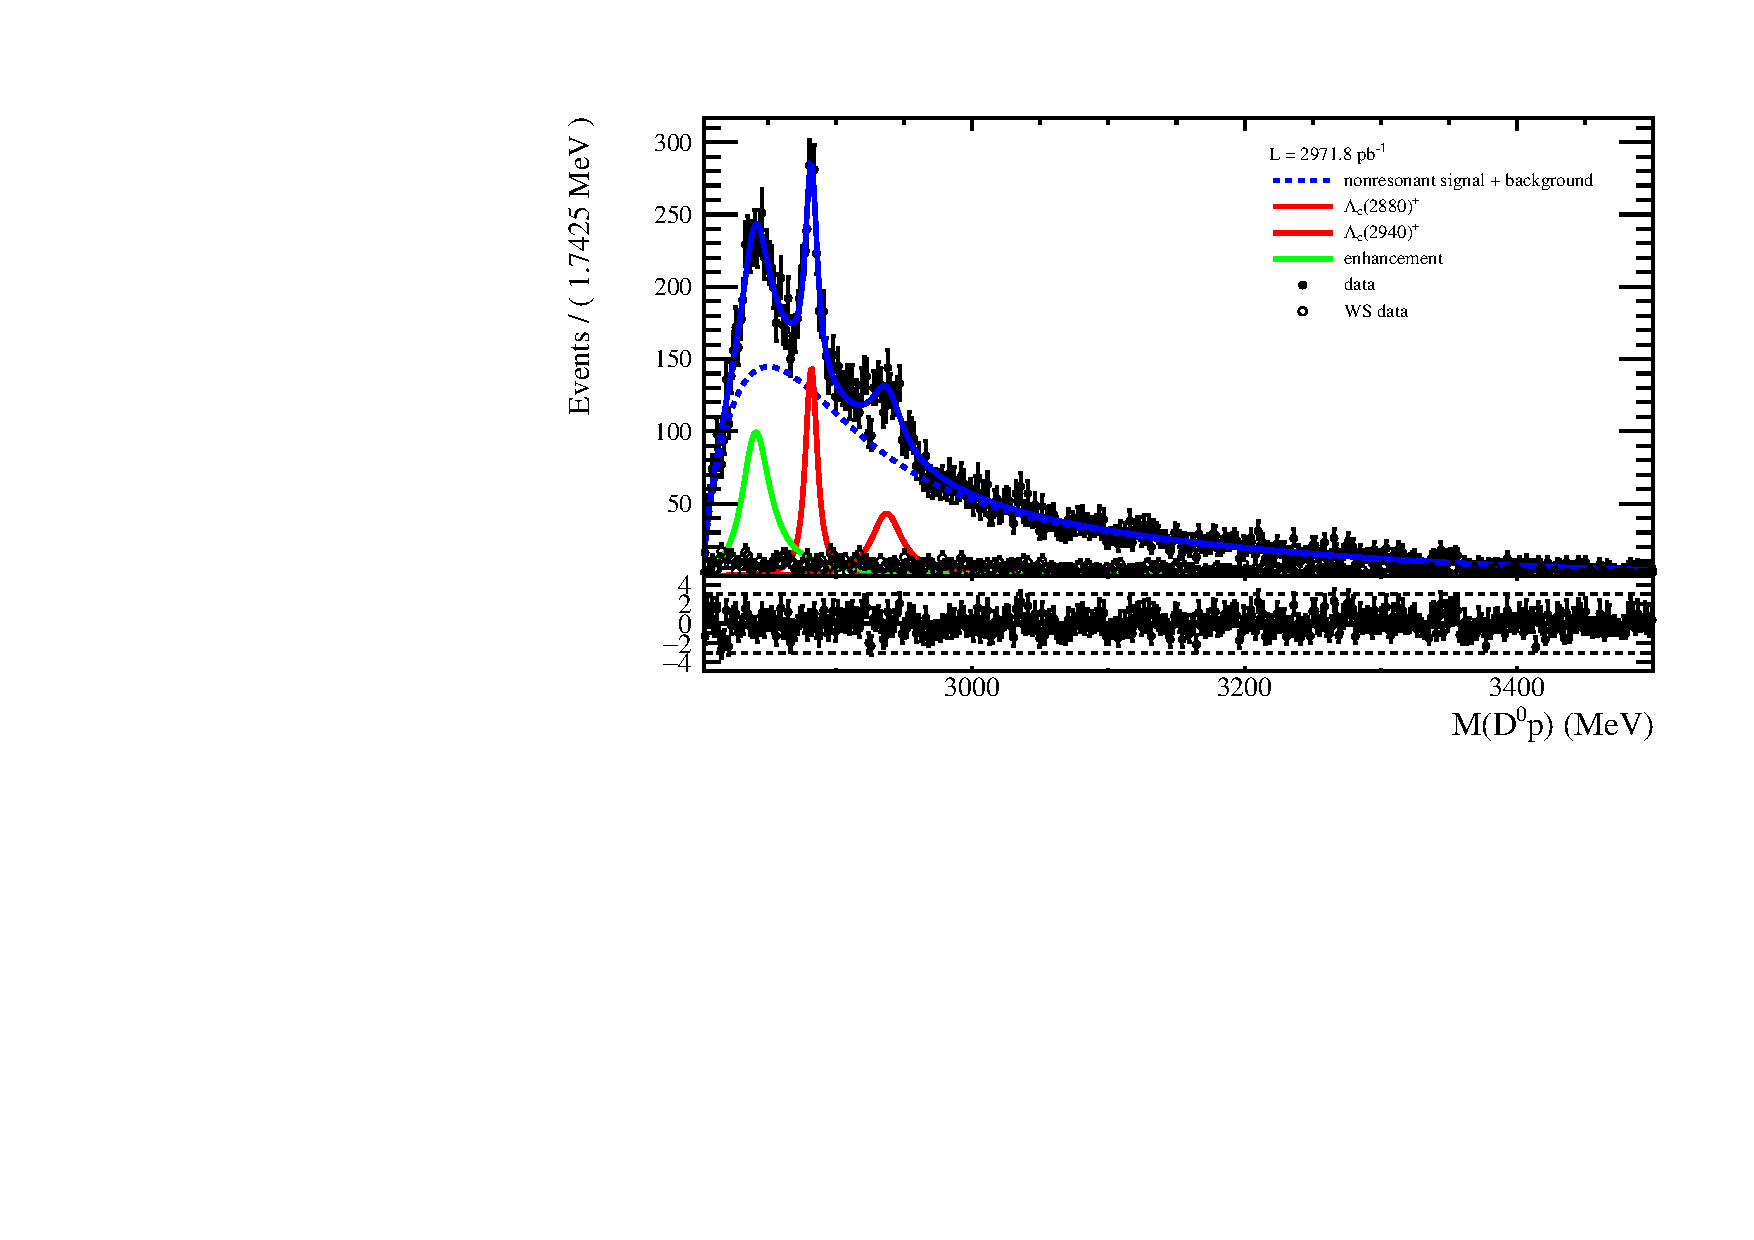
\includegraphics[width=\textwidth]{LbToD0p/fits/data/mD0p_RS/fit_TurnOnDExp_3RelBWPSRes}
	\caption{Invariant \Dz\proton mass distribution when requiring $\logIP < 1$. 
             The upper figure shows a fit with two resonances (red lines) for the \LcResI and \LcResII and a nonresonant part (blue dashed line). 
             Different attempts have been made to get a proper and converging fit, matching the data at low \Dz\proton mass, without success. 
             This issue can be solved by adding an additional resonant component (lower figure, green line), obeying the same fit model like the two resonances.}
    \label{fig:fit_mD0p_RS}
\end{figure}
 
\begin{table}[h]
    \centering
    \caption{Results of the \Dz\proton mass fit.}
    \label{tab:fit_mD0p_RS}
    $\begin{array}{lr@{\pm}l}
    \hline
    \text{Variable} & \multicolumn{2}{c}{\text{Value}} \\
    \hline
        \multicolumn{3}{l}{\text{\textbf{Yields}}} \\
\text{\LcResI signal yield}&(1.26 & 0.16) \cdot 10^{3}\\
\text{\LcResII signal yield}&(1.01 & 0.32) \cdot 10^{3}\\
\text{mass enhancement yield}&(2.12 & 0.44) \cdot 10^{3}\\
\text{nonresonant yield}&(1.65 & 0.08) \cdot 10^{4}\\
\multicolumn{3}{l}{\text{\textbf{\LcResI resonance}}} \\
\text{mean}&(2.88 & 0.00) \cdot 10^{3}\\
\text{width}&(8.90 & 1.40) \cdot 10^{0}\\
\multicolumn{3}{l}{\text{\textbf{\LcResII resonance}}} \\
\text{mean}&(2.94 & 0.00) \cdot 10^{3}\\
\text{width}&(2.62 & 0.79) \cdot 10^{1}\\
\multicolumn{3}{l}{\text{\textbf{Low mass enhancement}}} \\
\text{mean}&(2.84 & 0.00) \cdot 10^{3}\\
\text{width}&(2.44 & 0.37) \cdot 10^{1}\\
\multicolumn{3}{l}{\text{\textbf{nonresonant part}}} \\
\text{turn on mass threshold}&(2.80 & 0.00) \cdot 10^{3}\\
\text{turn on slope}&(-2.00 & 32.00) \cdot 10^{-5}\\
\text{exponential 1 slope}&(-2.34 & 0.13) \cdot 10^{-2}\\
\text{exponential 2 slope}&(-7.07 & 0.20) \cdot 10^{-3}\\
\text{fraction exponential 1}&(7.40 & 0.24) \cdot 10^{-1}\\

\hline
\end{array}$
\end{table}
    

\section{Determination of the mass resolution}
\label{sec:Massresolution}
Due to resolution effects, the width of a resonance in a mass spectrum can appear wider than its natural width.
In this analysis the effect is accounted for by convoluting the Breit-Wigner, which is assumed to be the natural shape of the resonance, with a double Gaussian, describing the smearing of the resonance due to finite mass resolution, see equation (\ref{eq:RES}).

The determination of the mass resolution is performed in a simulation by comparing the generated (also called ``true") mass with the reconstructed mass.
The mean of the mass difference distribution is expected to be zero and the width refers to the mass resolution.
The distribution is described by a double Gaussian function $f_1 \mathcal{G}(m|m_0,\sigma_1) + (1-f_1) \mathcal{G}(m|m_0,\sigma_2)$ to properly describe the broadening of the mass difference distribution in the tails.
To account for a potential mass dependence, this fit is performed in several bins of the true invariant \Dz\proton mass.
The left-hand side of Figure \ref{fig:massresolution} exemplarily shows the mass difference between reconstructed and generated mass together with the fit of a double Gaussian in the bin $2910 < M(\Dz\proton) < 2980 \mev$.
This bin corresponds to the \LcResII resonance.
The fits of all bins can be seen in Appendix \ref{app:Massresolution}, Figure \ref{fig:massresolution_all}.
The widths $\sigma_1$ and $\sigma_2$ and the fraction of the first Gaussian $f_1$ obtained by these fits in the respective bins are used for the parametrisation of the resonances in the nominal \Dz\proton mass fit as described by equation (\ref{eq:RES}).
Table \ref{tab:Massresolution} summarises the obtained values which are used for the further analysis.
Though there is a mass dependence of the resolution over the whole \Dz\proton mass spectrum it is assumed, that the mass resolution can be considered as constant over the natural width of the resonances.
\begin{table}[h]
    \centering
    \caption{Results of the fits to the mass difference distributions for the determination of the mass resolution. Only the values, which are required for the further analysis are quoted here.}
    \label{tab:Massresolution}
    $\begin{array}{lr@{\pm}lr@{\pm}lr@{\pm}l}
    \hline
    \text{Resonant component} & \multicolumn{2}{c}{\sigma_1 [\mev]} & \multicolumn{2}{c}{\sigma_2 [\mev]} & \multicolumn{2}{c}{f_1 [\mev]} \\
    \hline
    \LcResI   & \MassresResIwIval & \MassresResIwIerr & \MassresResIwIIval & \MassresResIwIIerr & \MassresResIfIval & \MassresResIfIerr \\
    \LcResII   & \MassresResIIwIval & \MassresResIIwIerr & \MassresResIIwIIval & \MassresResIIwIIerr & \MassresResIIfIval & \MassresResIIfIerr \\
    \text{enhancement} & \MassresStructurewIval & \MassresStructurewIerr & \MassresStructurewIIval & \MassresStructurewIIerr & \MassresStructurefIval & \MassresStructurefIerr \\
    \hline
    \end{array}$
\end{table}
The right-hand side of Figure \ref{fig:massresolution} shows the root-mean-square of the mass difference distributions in the different bins.
This serves as a measure for the mass resolution and how it evolves since it is hard to assign a single value for the mass resolution due to the fit of a double Gaussian.
At \Dz\proton mass threshold, the \Dz and the proton are at rest.
Thus, the measured \Dz\proton mass is just the sum of the PDG masses of the \Dz and the proton.
Hence, there is no sensitivity to a mass resolution at threshold.
If the measured \Dz\proton mass is above the threshold, there are contributions from the momenta of the \Dz and the proton to the measured \Dz\proton mass, too, influencing the mass resolution.
As the uncertainties of the momenta gets larger for increasing momenta, the mass resolution increases as well.
\begin{figure}[ptb]
    \centering
	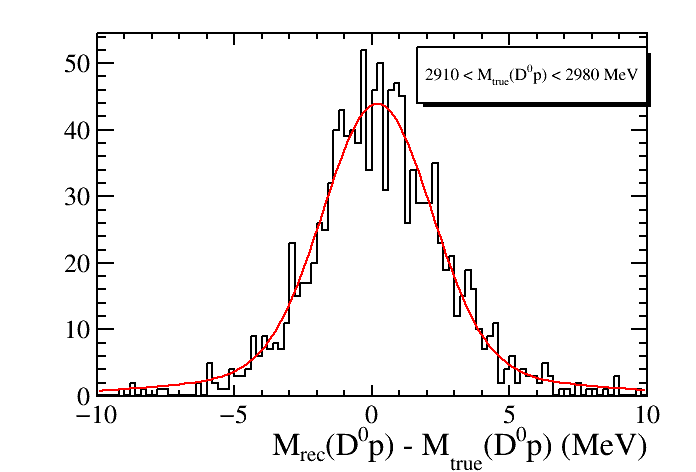
\includegraphics[width=0.49\textwidth]{LbToD0p/massresolution/massresolution_03}
	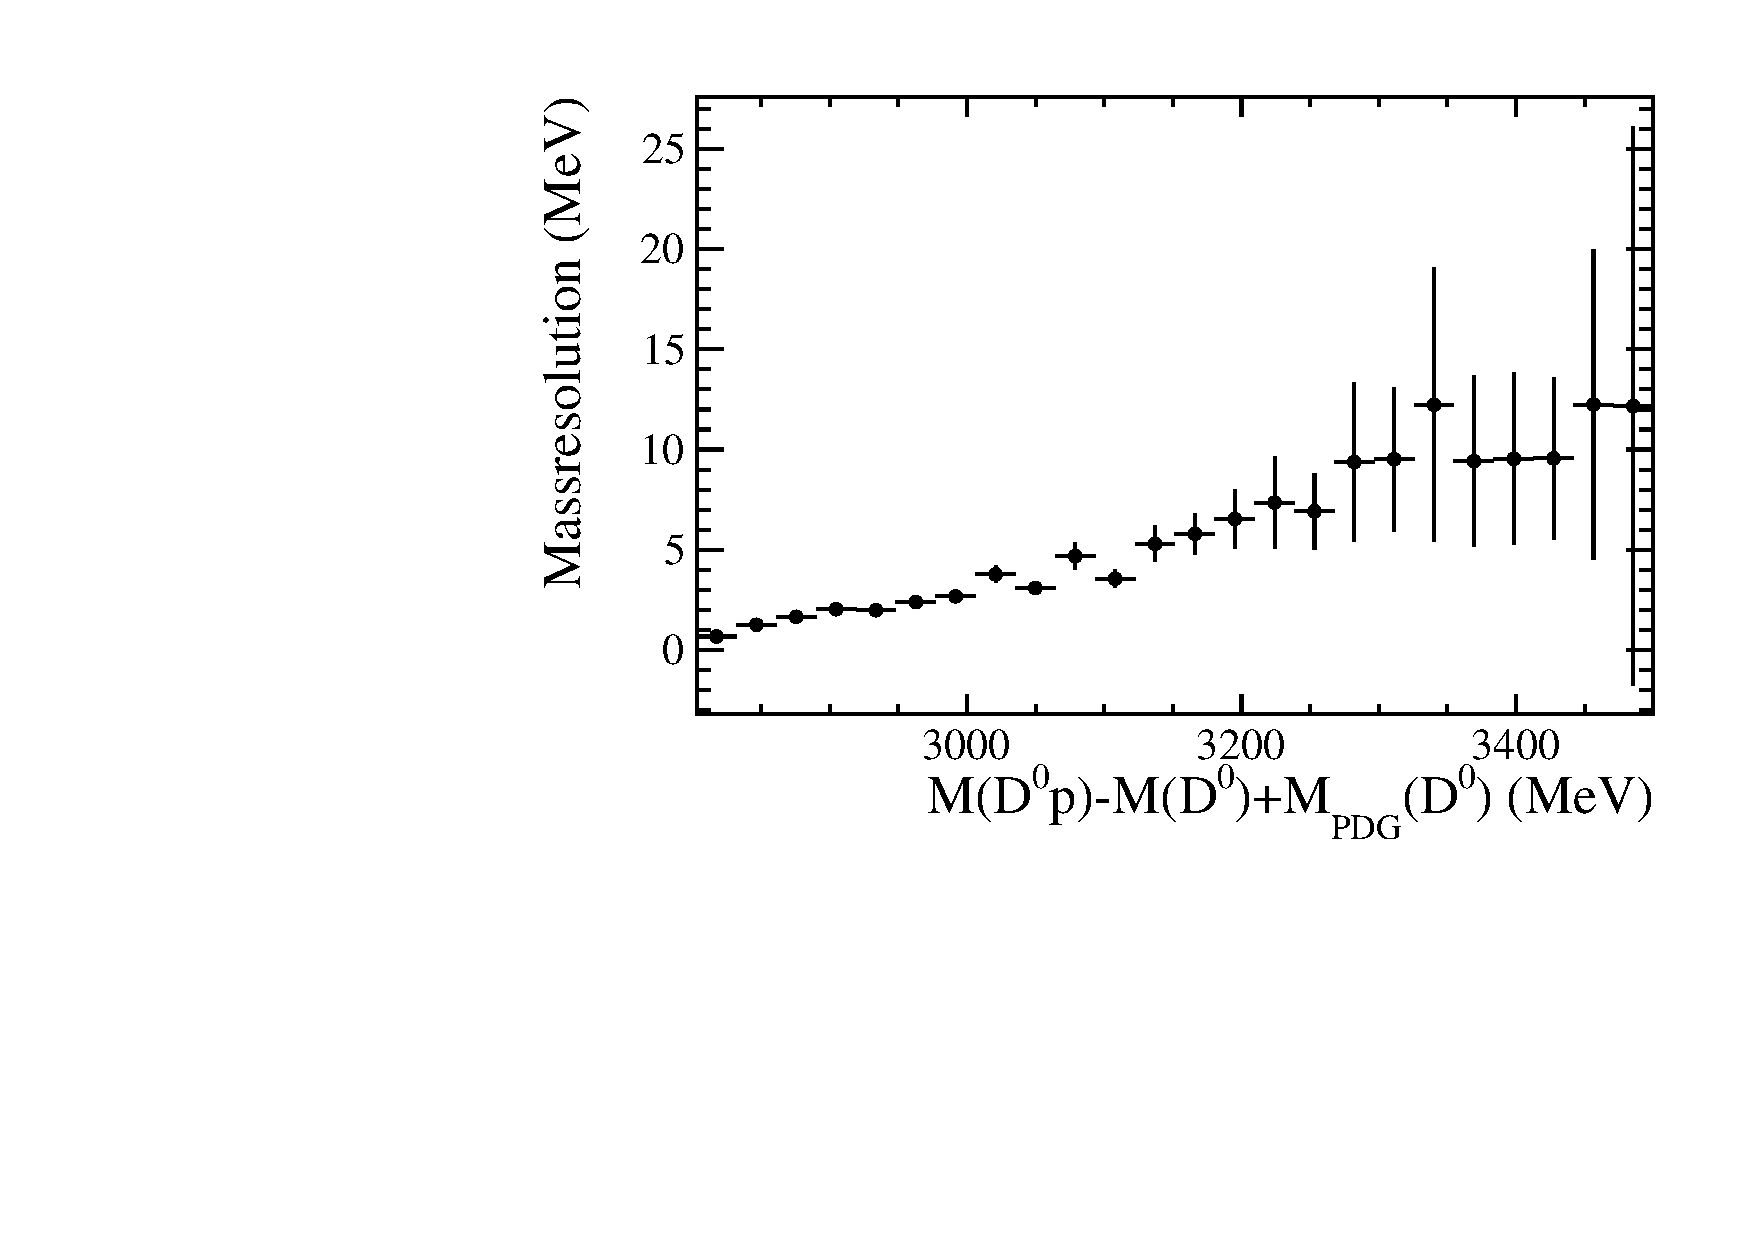
\includegraphics[width=0.49\textwidth]{LbToD0p/massresolution/massresolution_widths}
	\caption{Left: Fit of a Gaussian to the difference between generated and reconstructed \Dz\proton mass of the simulation sample in the range $2910 < M(\Dz\proton) < 2980 \mev$, corresponding to the bin of the \LcResII resonance. Right: root-mean-square (RMS) of the mass difference distributions for each bin.
    The RMS serves as a measure for the mass resolution since it is not easy to assign a single value for the mass resolution, since the distribution is modeled with a double Gaussian.}
    \label{fig:massresolution}
\end{figure}


\section{Nominal fit in two dimensions}
\label{sec:Fit_2D}
With a two-dimensional fit to the \Dz\proton mass and the \logIP distribution it is possible to distinguish between nonresonant signal and background in the \Dz\proton mass spectrum as already explained.
Thus, the different pieces of the previous sections are put together for a fit of both distributions.

It is assumed that the \logIP distribution is the same for all 4 different signal components (non-resonant signal, \LcResI, \LcResII, enhancement), since their decay topologies are the same\footnote{Presumed, that the enhancement indeed emerges to be a resonance or another signal component.}.
Hence, their \logIP distributions share all parameters. 
For the \logIP signal part a double Bifurcated Gaussian \DBfG is chosen, whereas the background is modeled by a CrystalBall function \CB.
The \Dz\proton mass' signal components are modeled with the same parametrisation as described in section \ref{sec:Shape_mD0p}. 
The empiric background function EBG is used to describe the background.
Thus, the total parametrisation $\mathcal{P}_\text{2D}$ of the two-dimensional \logIP/\MDp distribution is
\begin{align}
    & \mathcal{P}_\text{2D}(x, m | \vec{\lambda}) \propto \nonumber \\
    & \DBfG(x|x_{0, \text{sig}}, \vec{\sigma}_{\text{L,sig}}, \vec{\sigma}_{\text{R,sig}}, f_{\BfG_1}) \nonumber \\
    & \quad \cdot \left[\phantom{+} N_\text{nonres} \cdot \text{TDExp}(m|m_0, c_0, c_1, c_2, f_{c_1}) \right. \nonumber \\
    & \quad \phantom{\cdot [} + N_{\LcResI} \cdot \RES(m| m_{\LcResI}, m_1, m_2, \Gamma_{0, \LcResI}, \vec{\sigma}_{\LcResI}, f_{1, \LcResI}) \nonumber \\
    & \quad \phantom{\cdot [} + N_{\LcResII} \cdot \RES(m| m_{\LcResII}, m_1, m_2, \Gamma_{0, \LcResII}, \vec{\sigma}_{\LcResII}, f_{1, \LcResII}) \nonumber \\
    & \quad \phantom{\cdot [} + N_\text{enh} \cdot \RES(m| m_\text{enh}, m_1, m_2, \Gamma_{0, \text{enh}}, \vec{\sigma}_{\text{enh}}, f_{1, \text{enh}})\left.\right] \nonumber \\
    & + \CB(x| x_{0, \text{bkg}}, \sigma_\text{bkg}, \alpha, n) \cdot N_\text{bkg} \cdot \text{EBG}(m|m_0, m_1, m_2, p,c_{1, \text{bkg}}),
\end{align}
where $x$ denotes \logIP, $m$ the invariant \Dz\proton mass, $\vec{\lambda}$ the set of all fit parameters and $N_i$ the yields of the respective components.
All other parameters are explained in the sections before, where the different functions have been introduced.
All parameters are floating except for the mass resolution parameters of the resonant components in \RES(...) and the \Dz and proton mass ($m_1$ respectively $m_2$), that are required in the phase space function PS, which again is part of the relativistic Breit-Wigner and the empiric background function. 
The results of the fit are shown in Table \ref{tab:2Dfit} and the projections can be seen in Figure \ref{fig:fit2D}.
The model very nicely describes the data.
The pull distributions do not show any abnormalities.
A discussion of the result follows in section \ref{sec:Signalyield_D0p}.
\begin{figure}[ptb]
	\centering
	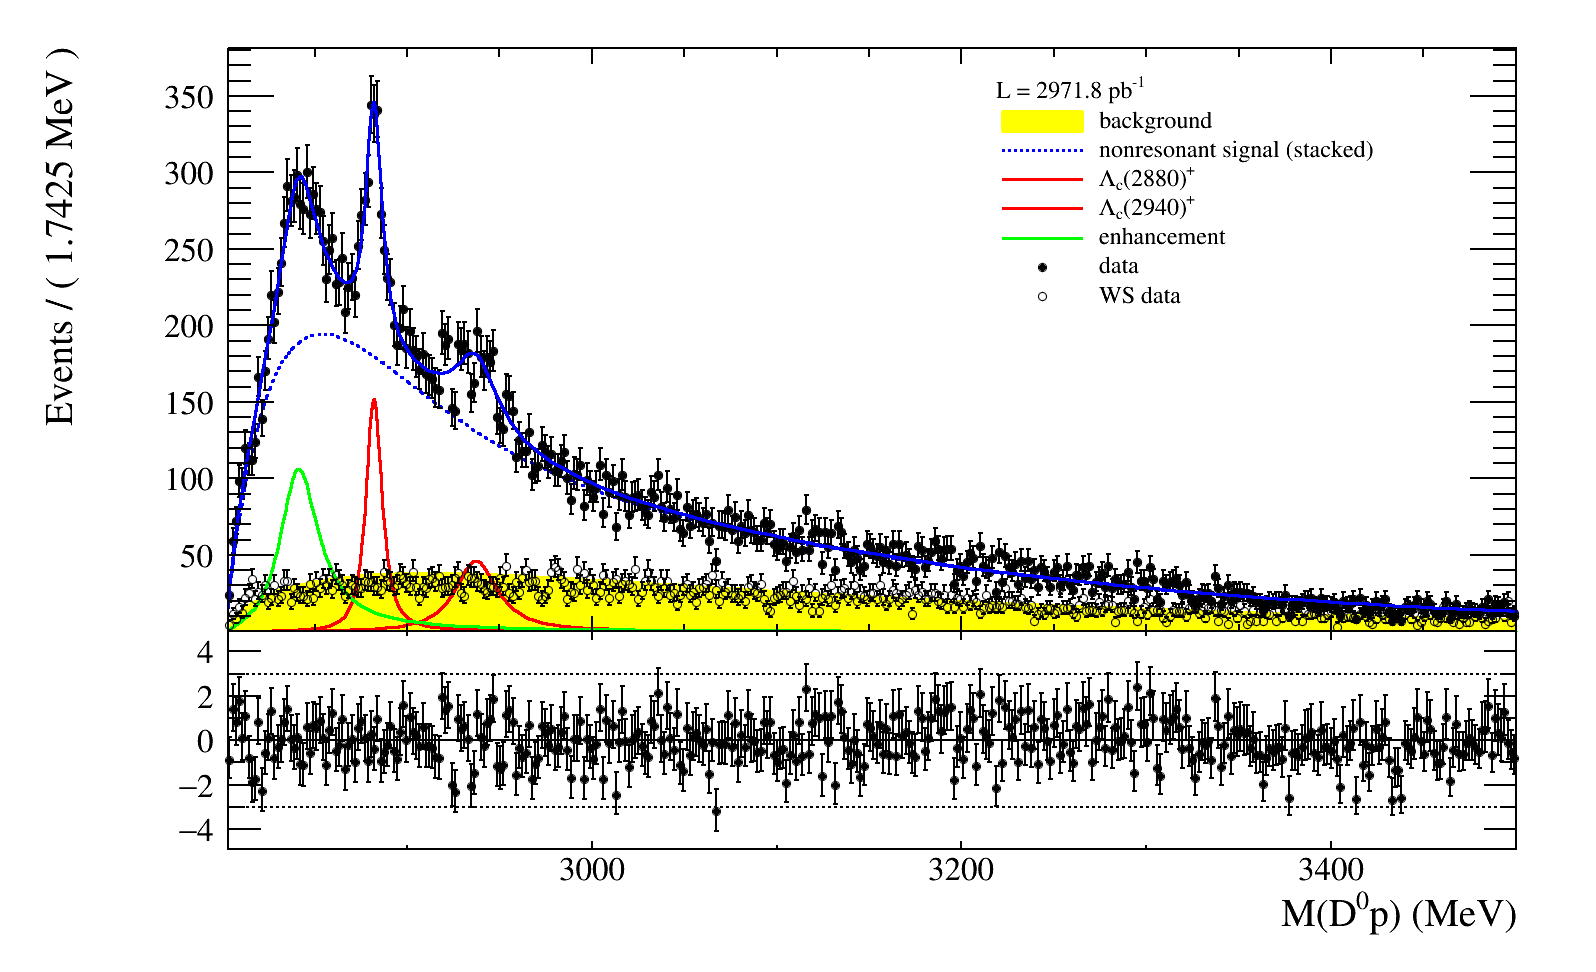
\includegraphics[width=\textwidth]{LbToD0p/fits/data/2Dfit/fit_DBfG_CB_vs_TurnOnDExp_3RelBWPSRes_EmpiricBG_mD0pProj} \\
	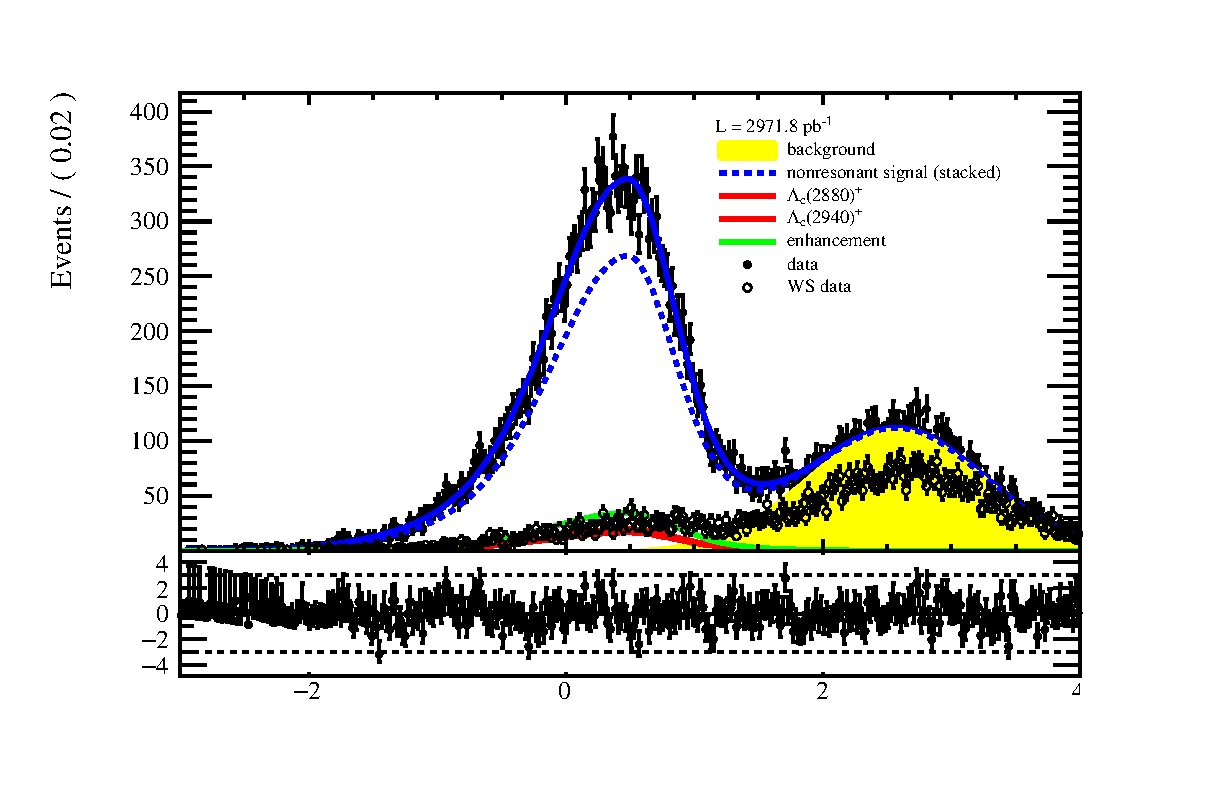
\includegraphics[width=\textwidth]{LbToD0p/fits/data/2Dfit/fit_DBfG_CB_vs_TurnOnDExp_3RelBWPSRes_EmpiricBG_logIPProj}
	\caption{Two-dimensional fit to the \LbToDpmunuX candidates. Top: projection of invariant \Dz\proton mass. Bottom: projection of \logIP distribution projection.
             The fit model is described in the text.
             The yellow shaded area shows the background component, stacked on top the non-resonant signal component marked as blue, dashed line.
             The two identified \LcResI and \LcResII resonances are drawn with a red solid line, the additional enhancement in green.
             For comparison the open circles show the wrong sign events.}
	\label{fig:fit2D}
\end{figure}
 
\begin{table}[h]
    \centering
    \caption{Results of the twodimensional M(\Dz\proton) and \logIP fit.}
    \label{tab:2Dfit}
    $\begin{array}{lr@{\pm}l}
    \hline
    \text{Variable} & \multicolumn{2}{c}{\text{Value}} \\
    \hline
        \multicolumn{3}{l}{\text{\textbf{Yields}}} \\
\text{\LcResI signal yield}&(1.28 & 0.15) \cdot 10^{3}\\
\text{\LcResII signal yield}&(1.06 & 0.24) \cdot 10^{3}\\
\text{mass enhancement yield}&(2.29 & 0.45) \cdot 10^{3}\\
\text{nonresonant signal yield}&(1.83 & 0.069) \cdot 10^{4}\\
\text{background yield}&(9.42 & 0.14) \cdot 10^{3}\\
\multicolumn{3}{l}{\text{\textbf{\LcResI resonance}}} \\
\text{mean [\mev]}&(2.88197 & 0.00034) \cdot 10^{3}\\
\text{width [\mev]}&(7.4 & 1.3) \cdot 10^{0}\\
\multicolumn{3}{l}{\text{\textbf{\LcResII resonance}}} \\
\text{mean [\mev]}&(2.9374 & 0.0016) \cdot 10^{3}\\
\text{width [\mev]}&(2.44 & 0.55) \cdot 10^{1}\\
\multicolumn{3}{l}{\text{\textbf{Low mass enhancement}}} \\
\text{mean [\mev]}&(2.84222 & 0.00088) \cdot 10^{3}\\
\text{width [\mev]}&(2.51 & 0.37) \cdot 10^{1}\\
\multicolumn{3}{l}{\text{\textbf{Nonresonant signal}}} \\
\text{turn on mass threshold [\mev]}&(2.80127 & 0.00057) \cdot 10^{3}\\
\text{turn on slope [\mev$^{-1}$]}&(-2.0 & 36.0) \cdot 10^{-4}\\
\text{exponential 1 slope [\mev$^{-1}$]}&(-2.34 & 0.14) \cdot 10^{-2}\\
\text{exponential 2 slope [\mev$^{-1}$]}&(-7.03 & 0.78) \cdot 10^{-3}\\
\text{fraction exponential 1}&(7.36 & 0.25) \cdot 10^{-1}\\
\multicolumn{3}{l}{\text{\textbf{Background (mass)}}} \\
\text{Empiric BG $c_1$ [\mev$^{-1}$]}&(-1.595 & 0.05) \cdot 10^{1}\\
\text{Empiric BG $p_0$}&(5.6 & 3.0) \cdot 10^{-2}\\
\multicolumn{3}{l}{\text{\textbf{Signal (\logIP)}}} \\
\text{mean}&(4.8 & 0.16) \cdot 10^{-1}\\
\text{left width 1}&(9.76 & 0.27) \cdot 10^{-1}\\
\text{right width 1}&(6.22 & 0.32) \cdot 10^{-1}\\
\text{left width 2}&(5.37 & 0.24) \cdot 10^{-1}\\
\text{right width 2}&(3.41 & 0.15) \cdot 10^{-1}\\
\text{fraction BfG 1}&(4.21 & 0.42) \cdot 10^{-1}\\
\multicolumn{3}{l}{\text{\textbf{Background (\logIP)}}} \\
\text{CB mean}&(2.573 & 0.012) \cdot 10^{0}\\
\text{CB $\sigma$}&(6.87 & 0.11) \cdot 10^{-1}\\
\text{CB $\alpha$}&(7.1 & 3.8) \cdot 10^{0}\\
\text{CB $n$}&(3.0 & 1.4) \cdot 10^{0}\\

\hline
\end{array}$
\end{table}
    

% ==================================
% Subsection: Control of the method
% ==================================
\section{Fit to the wrong sign proton data as cross-check}

As a cross-check the two-dimensionsal fit is performed for the wrong sign data with the same parametrisation as for the right sign data in section \ref{sec:Fit_2D}.
However, due to the absence of resonances it is purely described by the nonresonant functions, i.e. the nonresonant signal component and the background component.
The respective plots can be seen in Figure \ref{fig:fit_2D_WS}. 
No structure in the mass distribution is seen, especially the \LcResI and \LcResII resonances vanish in the wrong sign \Dz\proton.
Interesting is to note, that besides the two resonances even the enhancement vanishes.
Thus, it cannot be explained by random combinations of the particles.
Concerning the \logIP distribution, there is nevertheless a ``signal-like" part. 
This is presumably background from \BToDmunuX decays, where the $X$ is of ``wrong charge" and moreover misidentified as (anti)proton.
Since the physics are different for right sign and wrong sign events, the yield obtained in this WS fit cannot easily be subtracted from the nominal fit to account for fake proton backgrounds.
A more thorough study on fake backgrounds will be performed in Chapter \ref{sec:Backgrounds}.
\begin{figure}[ptb]
	\centering
	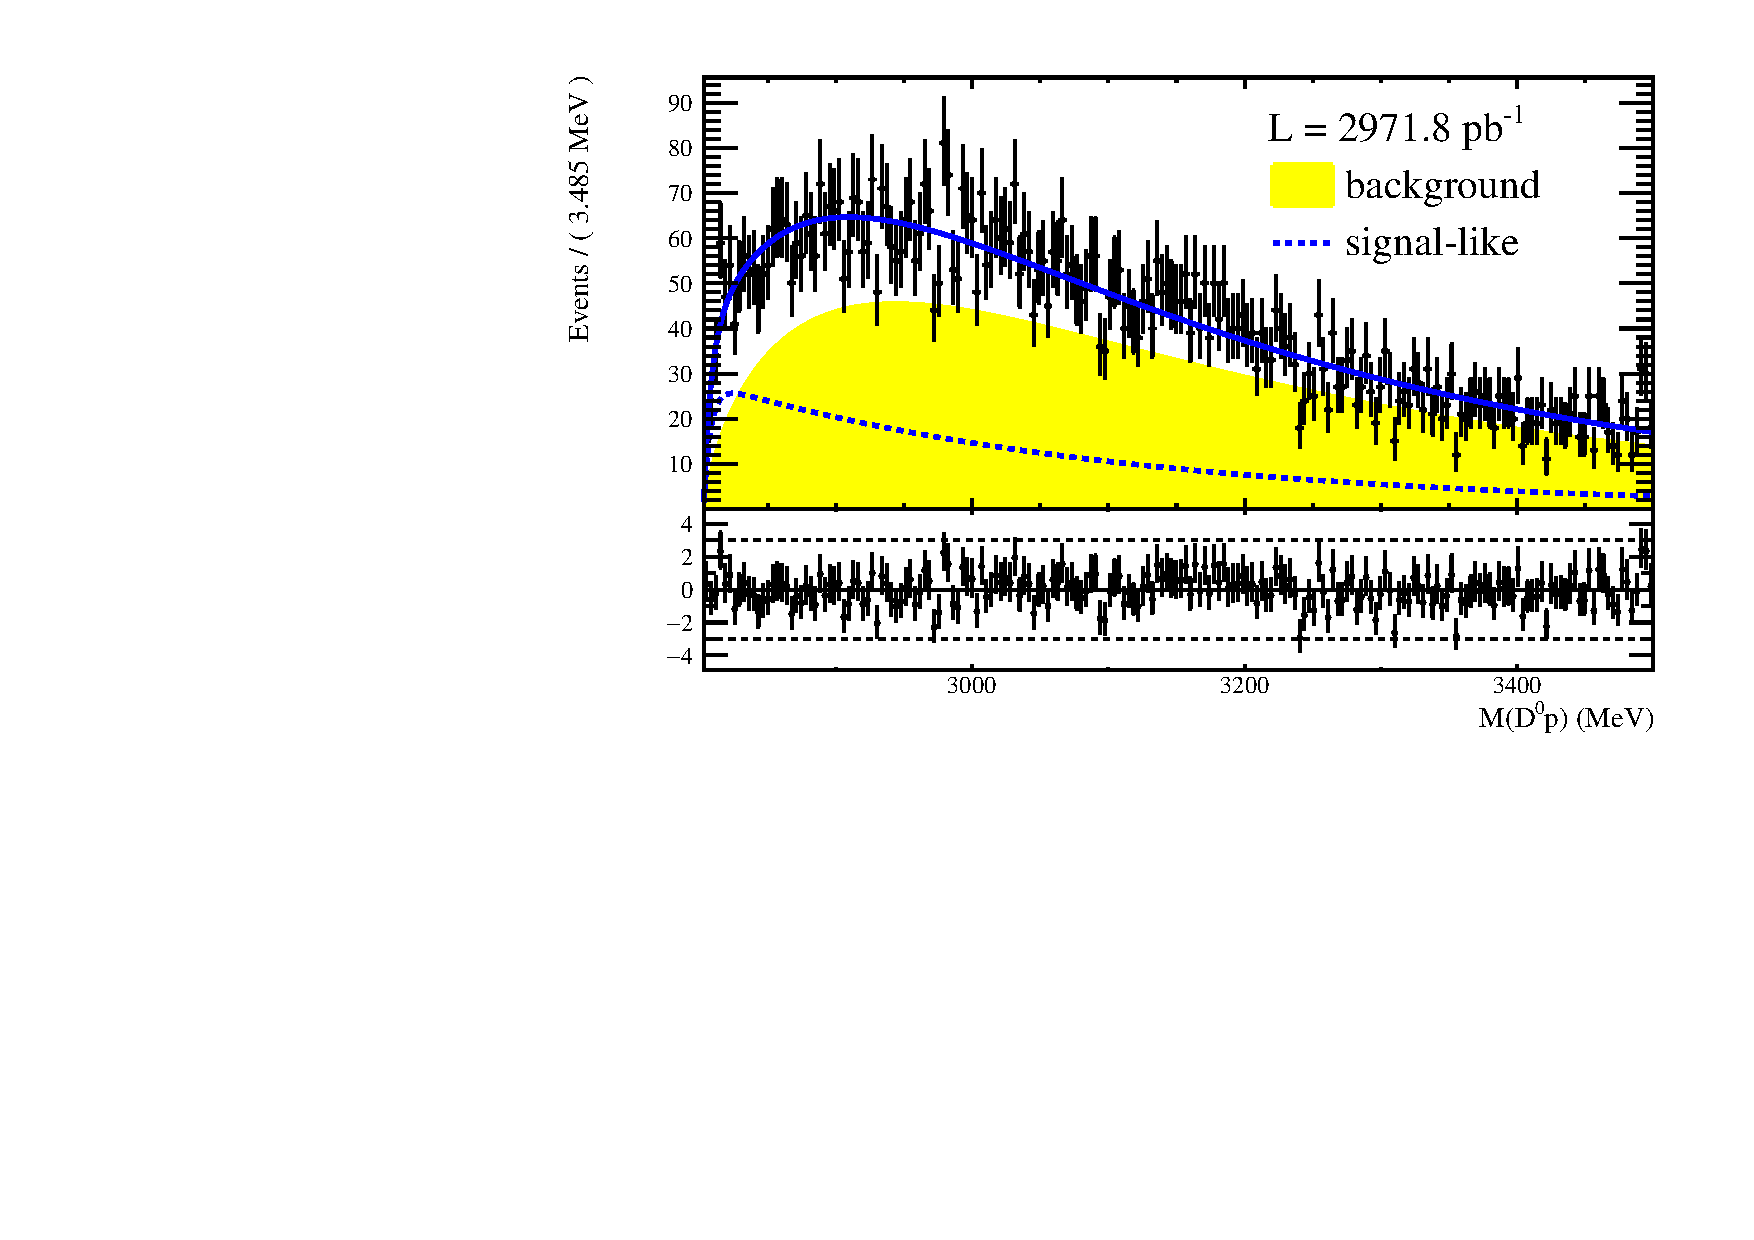
\includegraphics[width=0.49\textwidth]{LbToD0p/fits/data/2DWSfit/fit_DBfG_CB_vs_TurnOnDExp_EmpiricBG_mD0pProj}
	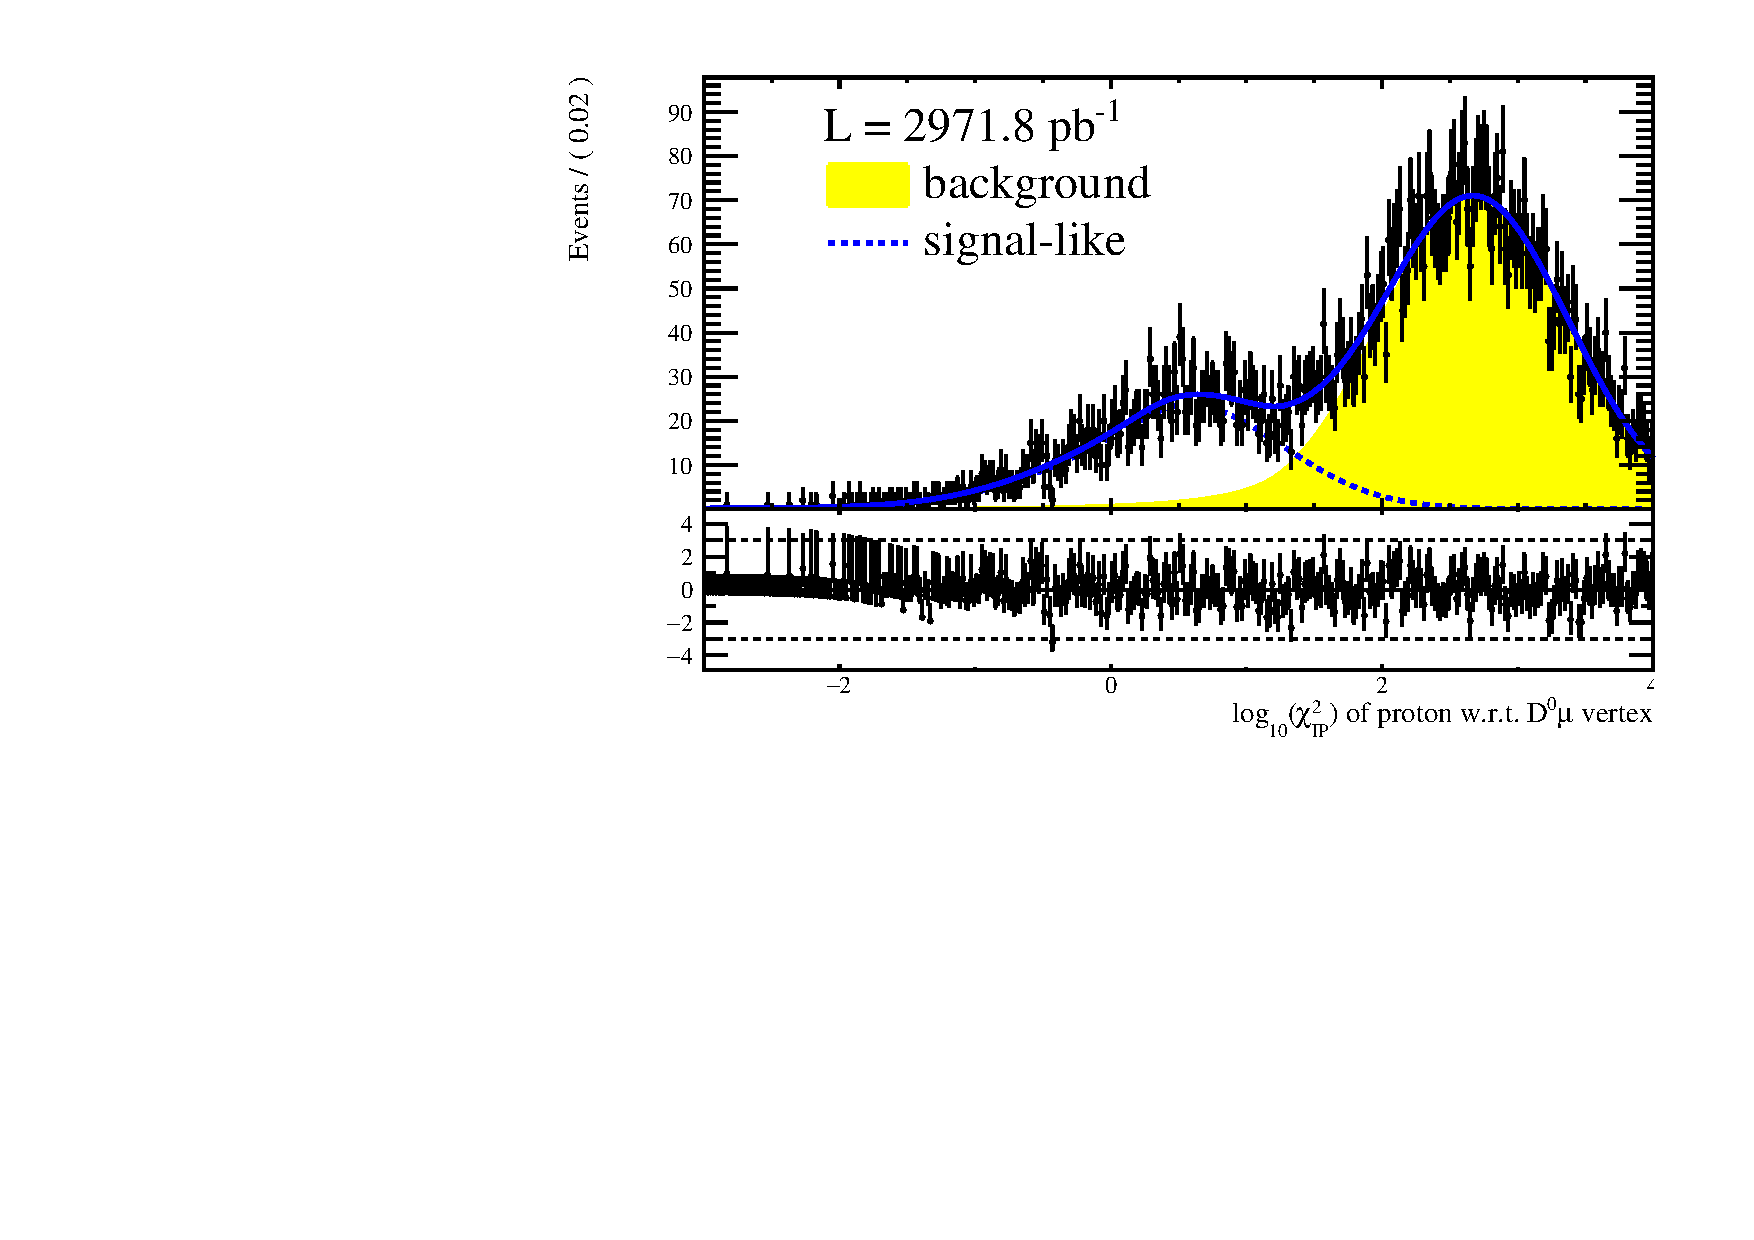
\includegraphics[width=0.49\textwidth]{LbToD0p/fits/data/2DWSfit/fit_DBfG_CB_vs_TurnOnDExp_EmpiricBG_logIPProj}
	\caption{Invariant \Dz\proton mass (left) and \logIP (right) distribution for ``wrong sign" (WS) events.
             The signal-like component (blue, dashed line) of the fit can be assigned to \BToDmunuX decays, where the $X$ is a fake proton of ``wrong" charge.}
	\label{fig:fit_2D_WS}
\end{figure}


% ==================================
% Section: Signal yield and resonances
% ==================================
\section{Extraction of \LbToDpmunuX signal yield together with \LcResI and \LcResII properties}
\label{sec:Signalyield_D0p}
From the previous fits different results can be obtained. 
The most important result is the \LbToDpmunuX signal yield \NDp for the determination of \R.
This result is obtained by the nominal two-dimensional fit.
The obtained yields for the non-resonant component, the \LcResI and the \LcResII as well as the enhancement, which can be found in Table \ref{tab:2Dfit} are summed up.
Thus, the total \LbToDpmunuX signal yield is
\begin{align*}
    \NDp &= N_{\text{nonres}} + N_{\LcResI} + N_{\LcResII} + N_{\text{enh}} \\
         &= (\NDpvalscient \pm \NDperrscient)\cdot 10^{\NDpexpscient}. 
\end{align*}
Remember, that the aim of this thesis is to measure the inclusive branching ratio of \LbToDpmunuX.
That is why all components ending up in a final state containing a \Dz, a proton and a muon are taken summed up for the total signal yield.
Again, it has to be confirmed in chapter \ref{sec:Structure}, that it is appropriate to consider the enhancement as signal.

As a side effect, the properties of the \LcResI and \LcResII resonances are extracted from the fit of the invariant \Dz\proton mass.
In this case it is not needed to distinguish between nonresonant signal and background, since only the peaks are of interest. 
To avoid uncertainties caused by this distinction, the properties of the two resonances are taken from the one-dimensional fit to the invariant \Dz\proton mass (see Table \ref{tab:fit_mD0p_RS}):
\begin{align*}
    \LcResI: \qquad  m_{\LcResI}       &= (\LcResImeanval \pm \LcResImeanerr) \mev, \\
                     \Gamma_{\LcResI}  &= (\LcResIwidthval \pm \LcResIwidtherr) \mev, \\
    \LcResII: \qquad m_{\LcResII}      &= (\LcResIImeanval \pm \LcResIImeanerr) \mev, \\
                     \Gamma_{\LcResII} &= (\LcResIIwidthval \pm \LcResIIwidtherr) \mev.
\end{align*}
The PDG values for the properties of the two resonances are $m_{\LcResI, \text{PDG}} = (2881.53 \pm 0.35)\mev$ and $\Gamma_{\LcResI, \text{PDG}} = (5.8 \pm 1.1)\mev$ for the \LcResI as well as $m_{\LcResII, \text{PDG}} = (2939.3^{+1.4}_{-1.5})\mev$ and $\Gamma_{\LcResII, \text{PDG}} = (17^{+8}_{-6})\mev$ for the \LcResII respectively.
These values are based on a \babar measurement of the \Dz\proton final state and a \belle measurement of \LcResI/\LcResII decays into $\Sigma_\cquark(2455)^{0,++}\pipm$ \cite{Belle_LcRes}.
The obtained results are in good agreement with the current world averages.

Though the reason for the low mass enhancement is not understood so far and it cannot be concluded if a new particle is seen, the obtained mass and width should be quoted here for the sake of completeness:
\begin{align*}
    \text{enhancement}: \qquad  m_{\text{enh}} &= (\Structuremeanval \pm \Structuremeanerr) \mev, \\
                                \Gamma_{\text{enh}}   &= (\Structurewidthval \pm \Structurewidtherr) \mev.
\end{align*}

	%\chapter{Normalisation fit}
\label{sec:Normalisationfit}
This chapter describes the analysis of the normalisation channel \LbToLcmunu (\LcTopKpi) resulting in the signal yield \NLc for the calculation of \R. The method is different to the one in the signal channel \LbToDpmunuX due to several reasons:
The final state particles of the subdecay \LcTopKpi are all reconstructed. 
It is thus possible to see a clear \Lc mass peak as shown in figure \ref{fig:plot_Lc_M}.
The small sidebands indicate a small combinatorial background concerning the subdecay \LcTopKpi.
Background coming from a random combination of a \Lc with a muon can be estimated by a look at the WS final states combinations \Lc\mup.
Since a \Lb can't decay into a \Lc\mup due to charge conservation, this unphysical combination gives a good hint for randomly combined \Lc\mun.
The second reason why a different method is chosen compared to the \LbToDpmunuX channel is the fact that the \Lb can decay in several excited \Lc states (in the following denoted as \Lcstar for any excited \Lc state).
It has been shown in \ref{SL_Vub} that the \LbToLcmunu data is saturated by the decays \decay{\Lb}{\LcstarRes{(2595)}\mun\neumb} and \decay{\Lb}{\LcstarRes{(2625)}\mun\neumb}.
These excited \Lcstar instantly decay for instance in \Lc\pip\pim. 
If these two pions aren't reconstructed, this decay can't be distinguished by its topology.
That's why a different approach for the determination of \NLc has to be chosen.
The solution of the latter problem is to fit the corrected \pKpi\mun, i.e the visible \Lb mass.
An explanation for this choice and the description of the fit is given in section \ref{sec:Normalisationfit}.
\begin{figure}[hptb]
    \centering
	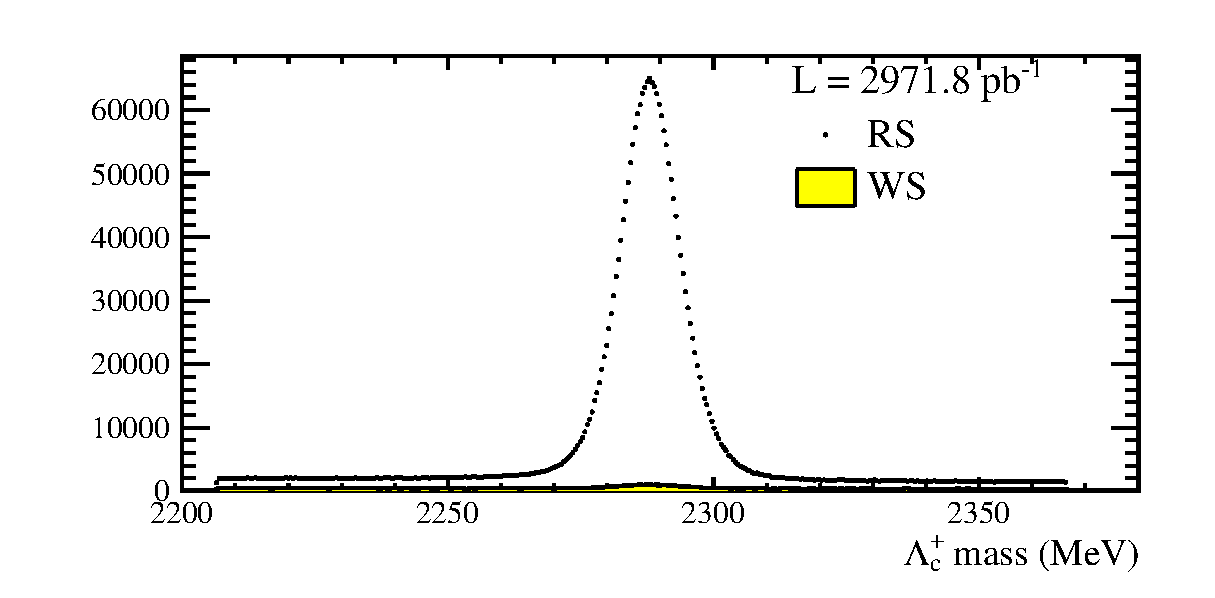
\includegraphics[width=\textwidth]{LbToLc/plots/data/Lc_M}	
	\caption{Plot of the invariant \pKpi mass. A clear mass peak identified as the \Lc can be seen. The yellow shaded area shows events with the WS combination \Lc\mup.}
	\label{fig:plot_Lc_M}
\end{figure}


\section{Reduction and handling of backgrounds}
This section describes the ways, how different sources of backgrounds are either handled or reduced.

\subsection{Non \Lc background}
As already mentioned the reconstructed \pKpi mass delivers a nice peak forming the hadronically decaying \Lc nicely seen in figure \ref{fig:plot_Lc_M}. 
Events being outside of this peak can be explained by a random combination of proton, kaon and pion and thus not being decay remnants of the \Lc.
Nonetheless there is also a certain amount of this ``combinatoric" background in the peak region.
It is statistically eliminated by a sideband subtraction (see section \ref{sec:Sidebandsubtraction}).
As signal band the invariant \pKpi masses in the range M(\pKpi) $\in \left[2260, 2320\right]\mev$ are chosen.
The background bands are M(\pKpi) $\in \left[2225, 2260\right]\mev$ or M(\pKpi) $\in \left[2320, 2345\right]\mev$.

\subsection{Random combinations of \Lc and \mun}
The next possible source of backgrounds are random combinations of \Lc and \mun. 
Due to the semileptonic decay \LbToLcmunu and hence the missing neutrino \neumb it is not possible to use a sidebandsubtraction on the invariant \pKpi\mun (\Lc\mun) mass.
Thus, wrong sign (WS) events, i.e. ``unphysical" events with a \Lc\mup in the final state as explained above are used to estimate the amount of random \Lc\mun background.
While trying to perform the final fit later (see sec. \ref{sec:FitCorrectedMass}) it turns out, that the number of WS events is too small that the fit is sensitive to it.
As a consequence it is assumed that the shape and the number of the WS events are equal to the shape and number of random \Lc\mun combinations.
Finally, the WS events are subtracted from the ``right sign" (RS) events to eliminate this source of backgrounds.

\subsection{Peaking backgrounds}
The third source of backgrounds is peaking background from partially reconstructed decays. 
In this case the data is saturated by the decays \decay{\Lb}{\LcstarRes{(2595)}\mun\neumb} and \decay{\Lb}{\LcstarRes{(2625)}\mun\neumb} \cite{SL_Vub}.
The \Lcstar subsequently decay in a \Lc and an untracked neutral remnant, e.g. \piz, \pip\pim.
Since this decay happens instantly it looks the same as \LcTopKpi in the detector.
The solution is to fit the corrected \pKpi\mun (alias the visible \Lb) mass. 
A property of the corrected mass is that if the only missing particle is a massless, then the corrected mass should peak around the real mass of the mother particle, here the \Lb.
If there are additionally more missing, but massive particles then this peak should be shifted to lower masses.
It is thus expected that the corrected \pKpi\mun mass distributions look different for the semileptonic \Lb decays into a \Lc, \LcstarRes{(2595)} and \LcstarRes{(2625)}.
A fit of the corrected mass should also be able to distinguish between those components.

\section{Fit of the \pKpi\mun corrected mass}
\label{sec:FitCorrectedMass}
Having read the previous sections it should be clear, why the corrected \pKpi\mun mass is used for the determination of \NLc, the \LbToLcmunu signal yield.
Nonetheless it should be verified, that the corrected \pKpi\mun mass is an appropriate variable.
Therefore simulations for the different components, \LbToLcmunu, \decay{\Lb}{\LcstarRes{(2595)}\mun\neumb} and \decay{\Lb}{\LcstarRes{(2625)}\mun\neumb} are used to compare their corrected \pKpi\mun mass shapes.
\begin{figure}[hptb]
	\centering
	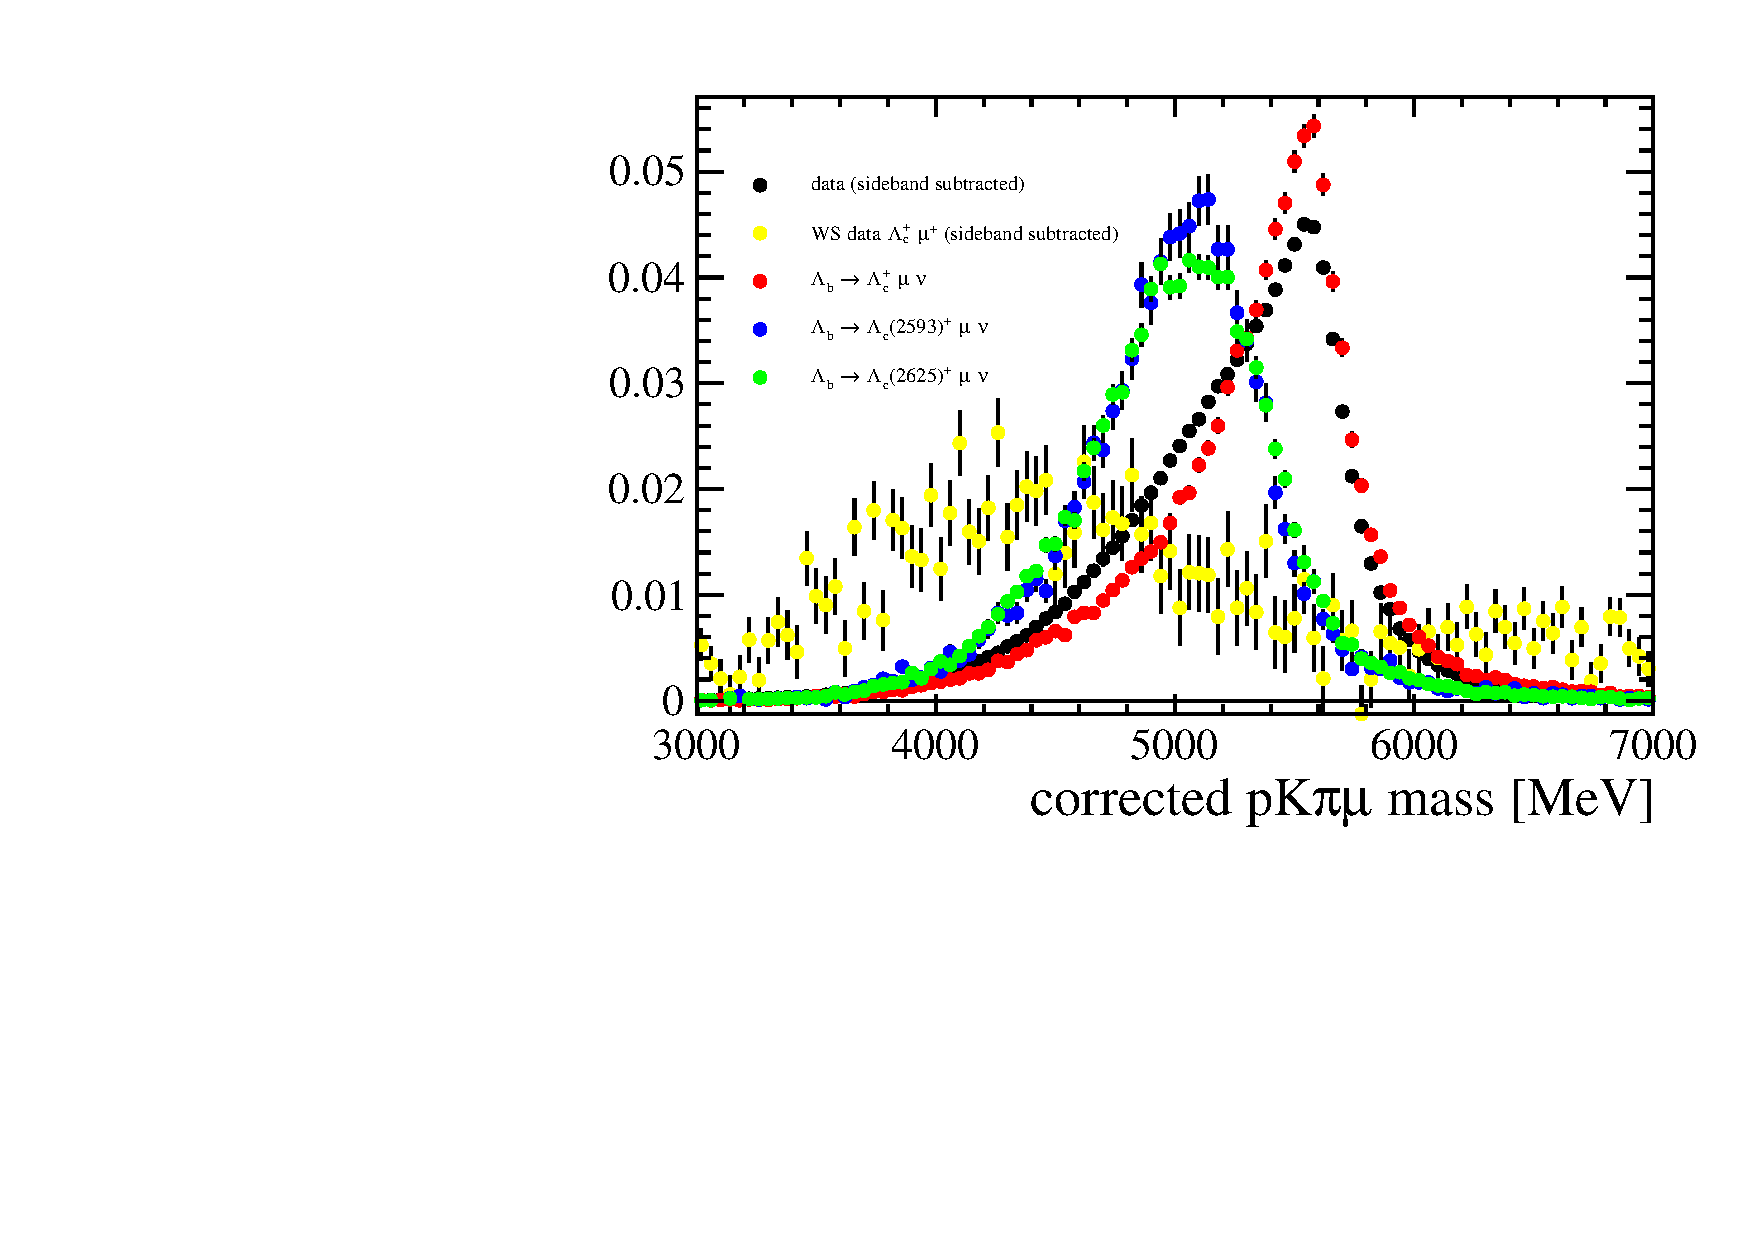
\includegraphics[width=0.49\textwidth]{LbToLc/correctedMass/correctedMass}
	\caption{Comparison of the \pKpi\mun corrected mass for the semileptonic \Lb decays via \Lc, \LcstarRes{(2593)} and \LcstarRes{(2625)} gained from simulation. The black points show the sideband subtracted data distribution. The shape of combinatorial \Lc\mun background (WS events) is shown in yellow.}
	\label{fig:correctedMass_normalisation}
\end{figure}

From figure \ref{fig:correctedMass_normalisation} one can draw the following conclusions:
\begin{itemize}
    \item The corrected \pKpi\mun mass indeed looks different for \Lc and \Lcstar channels.
    \item It is not possible to distinguish between the \LcstarRes{(2595)} and \LcstarRes{(2625)} as their shapes are too similar.
\end{itemize}
The latter conclusion isn't really a problem since the only result of interest is the \LbToLcmunu signal yield. 
A distinction among the excited states isn't needed.
In the fit there will be just a component for both final states.
Having these in mind, the fit procedure is done as follows:
\begin{enumerate}
    \item The data is subtracted by the \pKpi (i.e. \Lc) mass bands.
    \item The corrected \pKpi\mun mass distribution is subtracted by the WS events' distribution.
    \item A fit of the \pKpi\mun mass is performed using the Beeston-Barlow method (see sec. \ref{sec:BeestonBarlow}) to account for uncertainties in the MC corrected mass templates. The fitted components are the \Lc signal yield and one for both excited \Lcstar channels.
    \item For the plotting (see fig. \ref{fig:correctedMass_fit} and a better comparison the WS component is added again.
\end{enumerate}
The results can be seen in figure \ref{fig:correctedMass_fit} and table \ref{tab:fit_correctedMass}. The \LbToLcmunu signal yield \NLc, required for the determination of \R is:
\begin{align*}
    \NLc = (\NLcvalscient \pm \NLcerrscient)\cdot 10^{\NLcexpscient}
\end{align*}
\begin{figure}[hptb]
	\centering
	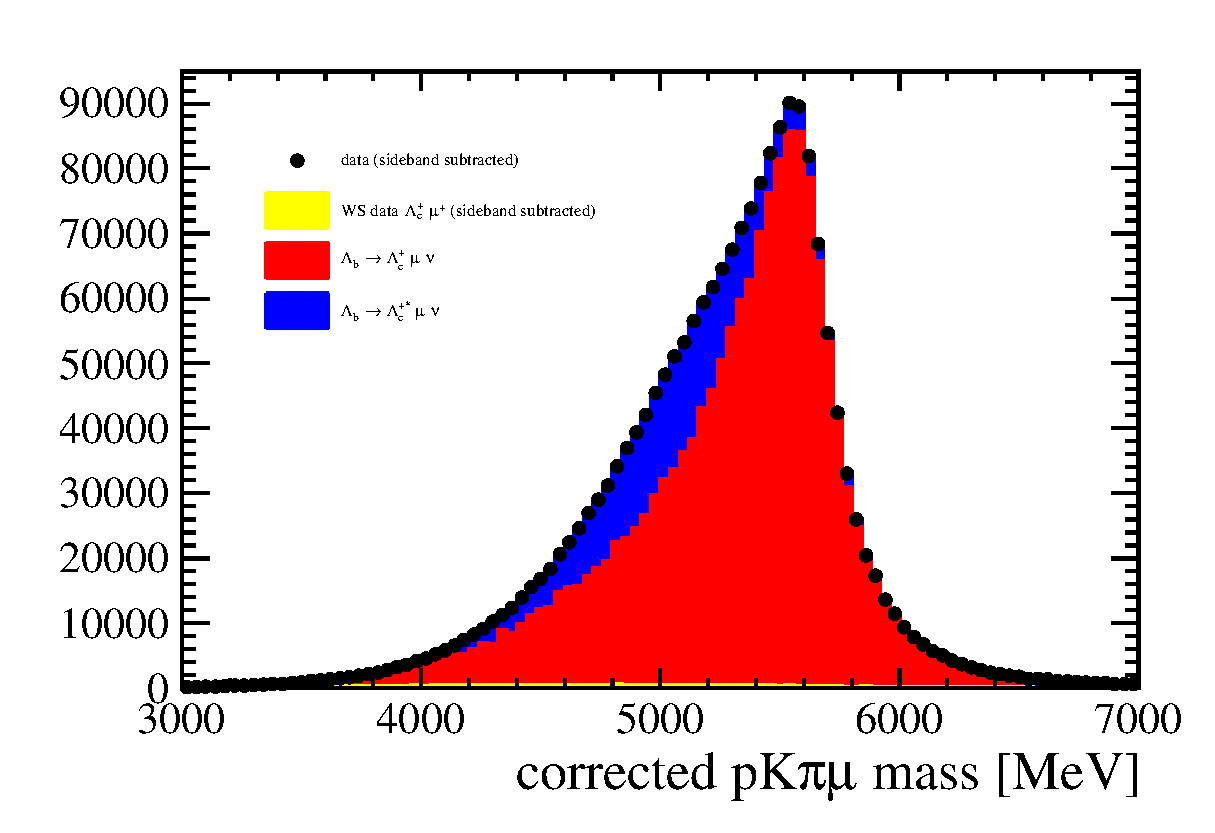
\includegraphics[width=0.49\textwidth]{LbToLc/correctedMass/fit_correctedMass}
	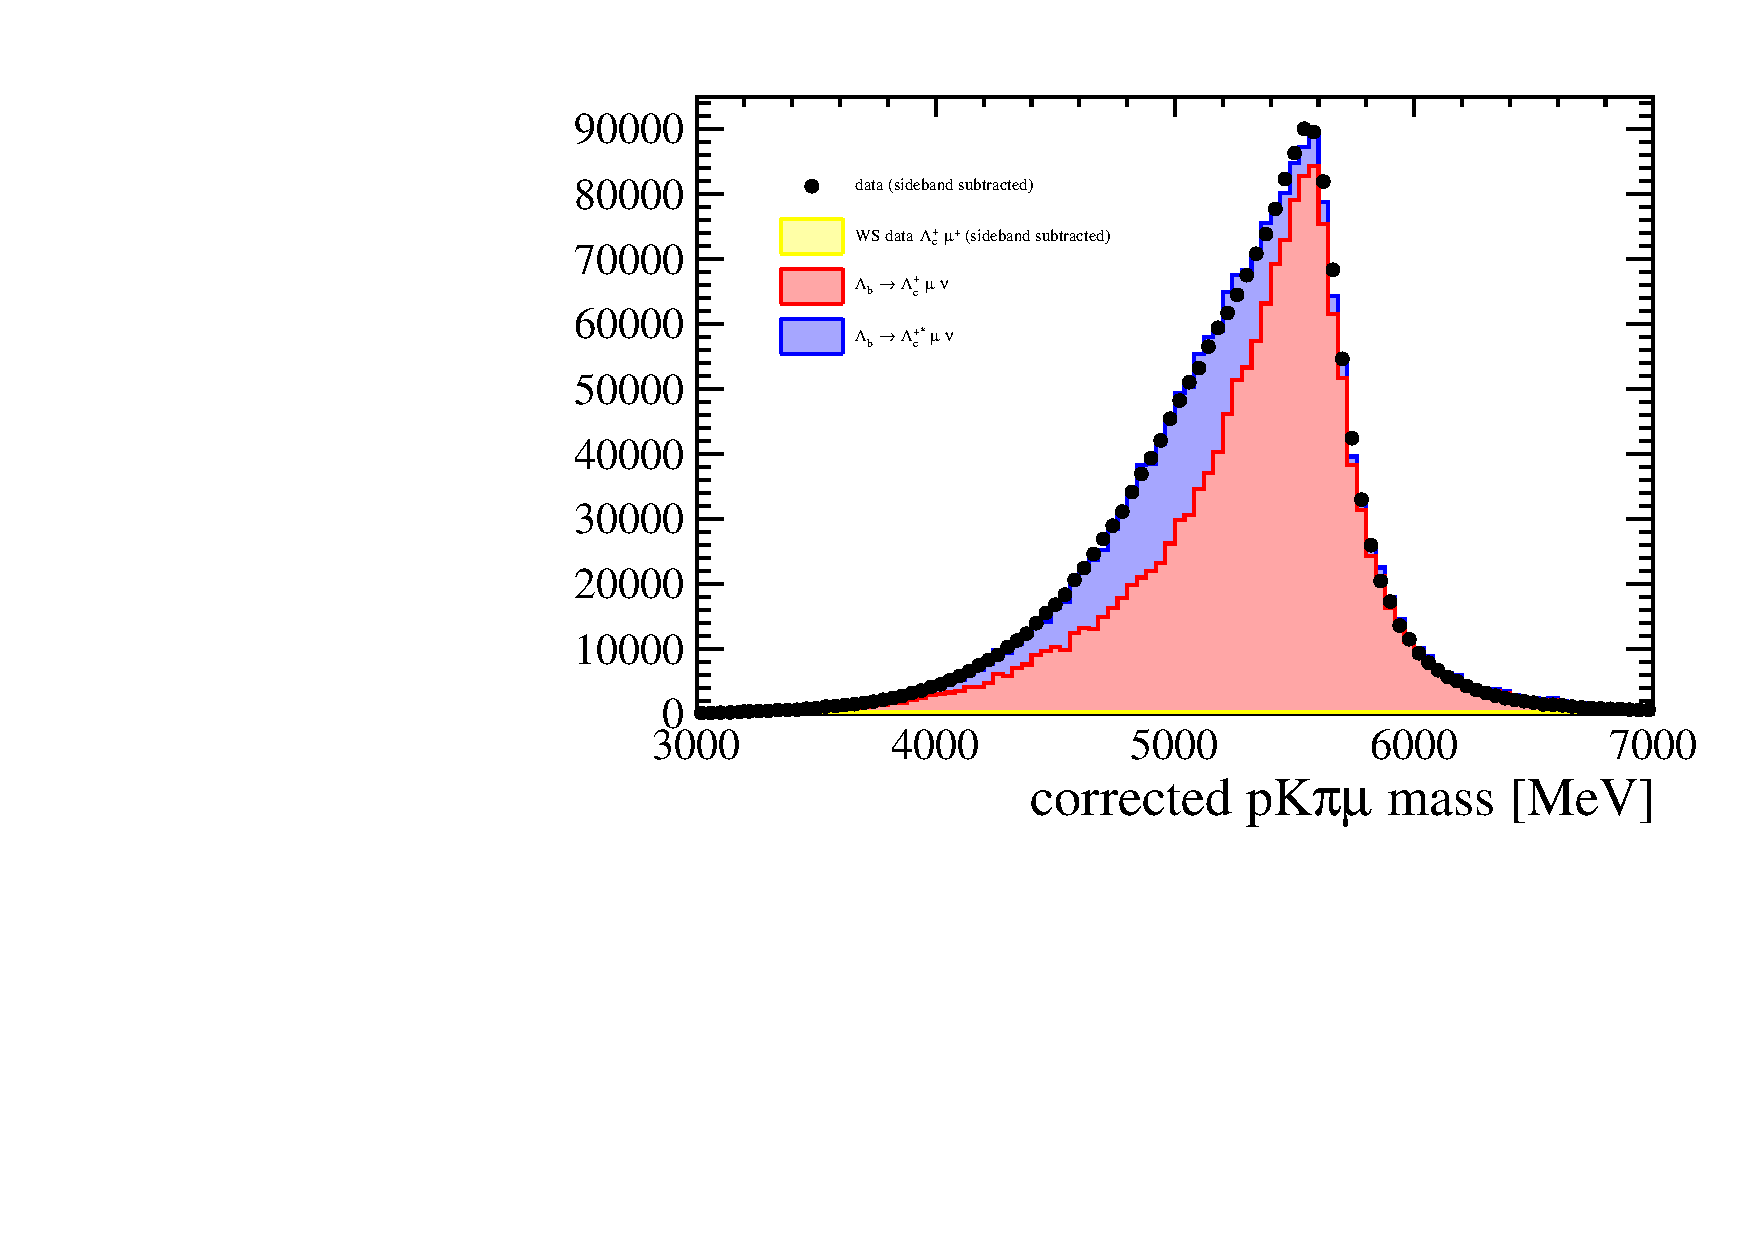
\includegraphics[width=0.49\textwidth]{LbToLc/correctedMass/fit_correctedMass_noBB} \\
	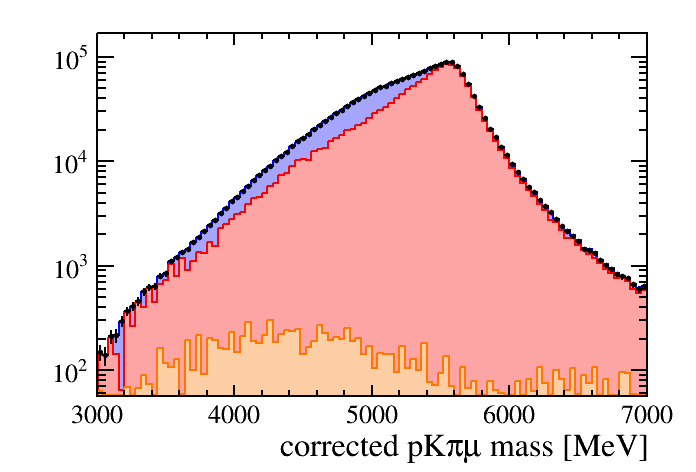
\includegraphics[width=0.49\textwidth]{LbToLc/correctedMass/fit_correctedMass_logscale}
	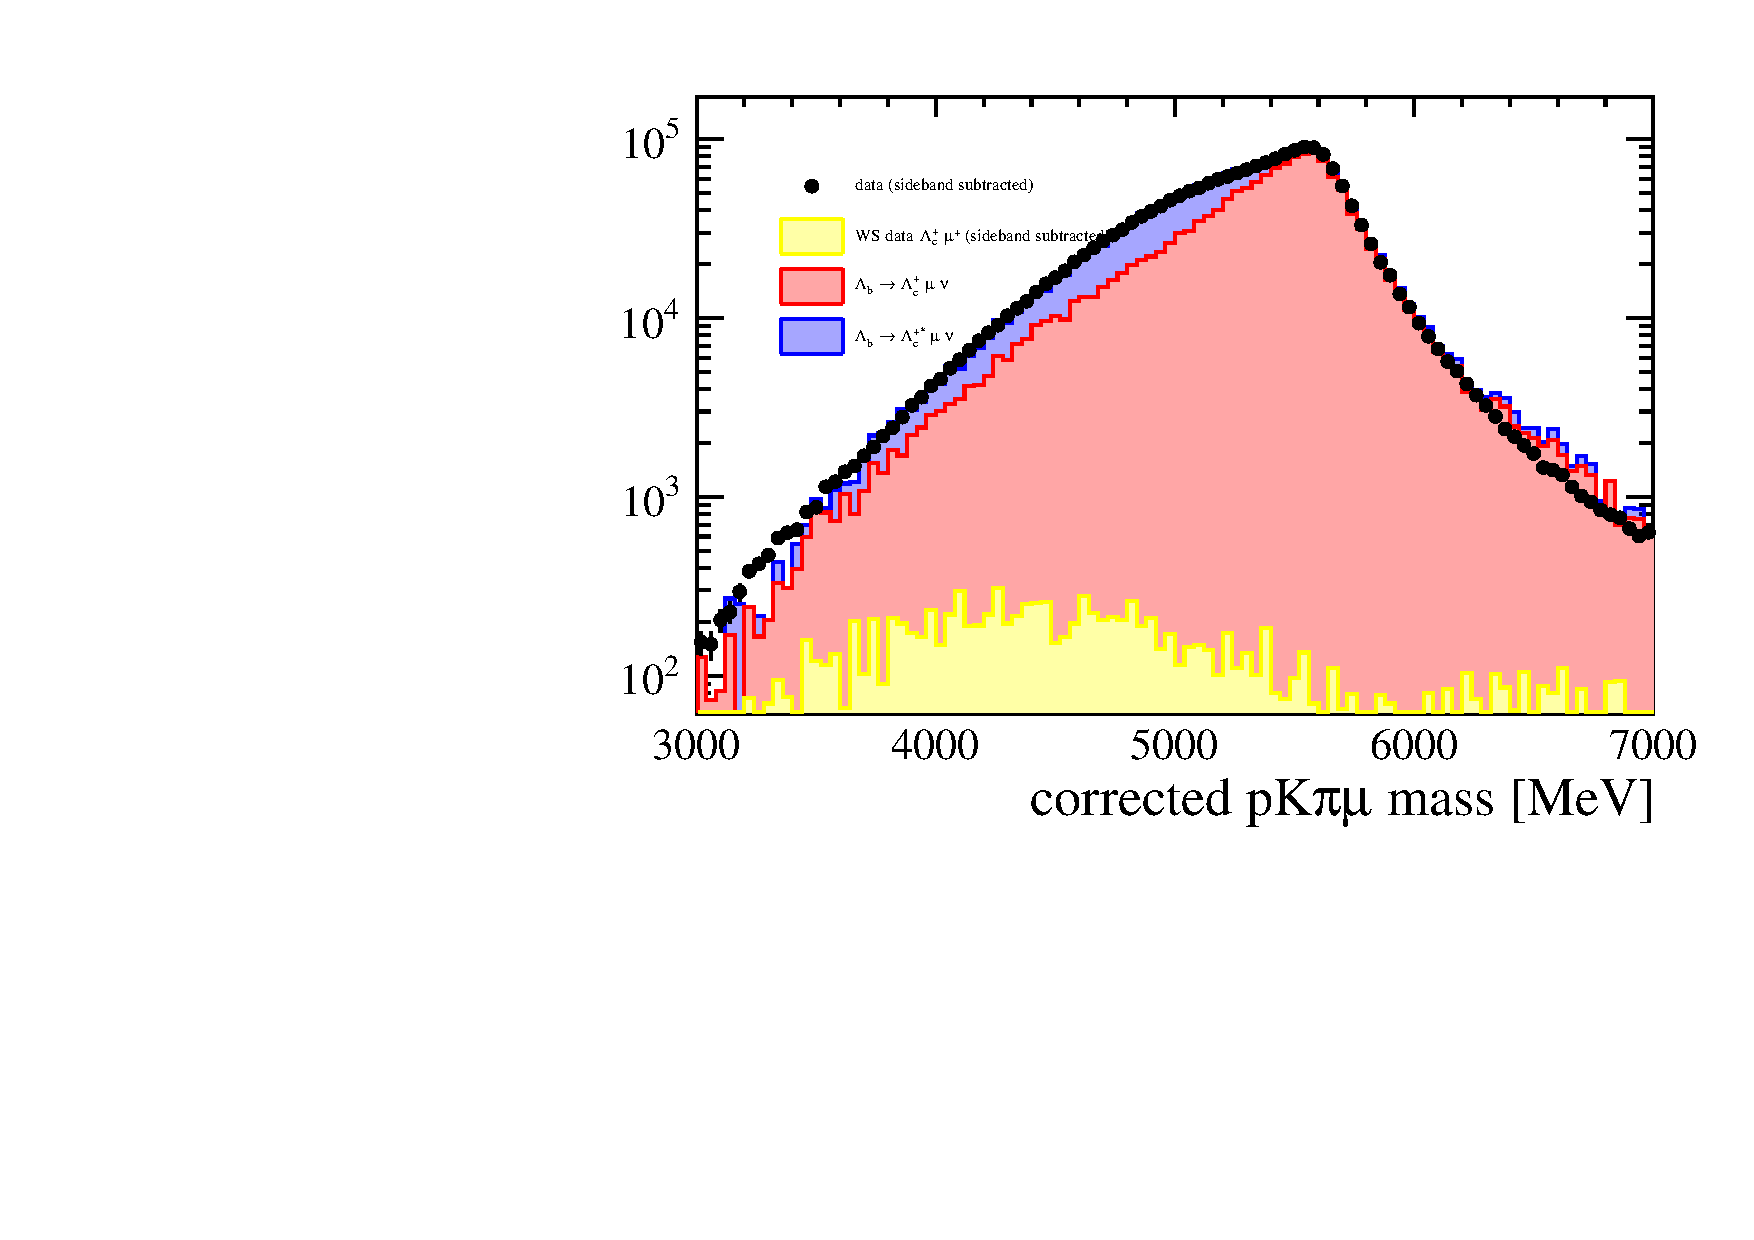
\includegraphics[width=0.49\textwidth]{LbToLc/correctedMass/fit_correctedMass_noBB_logscale}
	\caption{Fit to the \pKpi\mun corrected mass for the determination of the \LbToLcmunu signal yield. The left plot shows the fitresult with the Beeston-Barlow adjusted templates, the right one the bare templates without any modification. The top row shows the result on a linear, the bottom row on logarithmic scale.}
	\label{fig:correctedMass_fit}
\end{figure}

 
\begin{table}[h]
    \centering
    \caption{Results of the \Lc corrected mass fit.}
    \label{tab:fit_correctedMass}
    $\begin{array}{lr@{\pm}l}
    \hline
    \text{Variable} & \multicolumn{2}{c}{\text{Value}} \\
    \hline
        \text{\Lc candidates \NLc}&(1.544 & 0.011) \cdot 10^{6}\\
\text{excited \Lcstar candidates}&(4.375 & 0.096) \cdot 10^{5}\\
\text{combinatoric background}&(1.196 & 0.033) \cdot 10^{4}\\

\hline
\end{array}$
\end{table}
    

	%\chapter{Efficiencies}
\label{sec:Efficiencies}

The detection and reconstruction of particle decys is not perfect at all, i.e. not all particles and tracks happening in succession of a \proton\proton interaction are detected and recorded.
This discrepancy between the measured signal yields and the actually happened decays is summarized with the term ``efficiencies".
There are several reasons why different kinds of efficiencies occur.
Here are some examples:
\begin{itemize}
    \item Particles are flying out of the detector.
    \item A particle traverses a sensor in the deadtime, i.e. a signal caused by an earlier particle is still processed. 
          In this time, the sensor isn't able to process the second signal.
    \item Applying cuts for the reduction of background prevents signal events to pass these cuts as well
    \item ...
\end{itemize}
It's obvious that this list above is only the tip of the iceberg.
Nonetheless it's crucial to account for these efficiencies if one measures a physical quantity reliant on the number of events.
The way how the efficiencies for the \LbToDpmunuX and \LbToLcmunu enter the measurement of the relative branching ratio \R is shown in equation (\ref{eq:R}).

The determination of the efficiencies requires the use of simulations.
These simulation samples contain informations about all generated events as well as reconstructed events after the simulation of the detector. 
The naive way would be to divide the number of reconstructed MC events after applying all selection cuts and divide this by the number of generated events. 
This efficiency is hereafter called selection efficiency \effSel.
Nonetheless, the generation of the events isn't efficient at all. 
Several requirements are already applied during generation to reduce the computation time of the simulation production.
Above all the simulation of the detector takes a lot of time.
That's why all generated events are required to be in the \lhcb aceptance.
A further acceleration of the production process can be achieved with additional requirements on the final state particles' (transverse) momenta.
Concerning the \LbToDpmunuX and \LbToLcmunu channel these requirements are different and likewise the efficiencies of the generation process.
Thus, the so called generator level efficiency \effGen also has to determined for both channels. 
The total efficiency used for the calculation of \R is then the product $\effGen \cdot \effSel$.

As life is not that easy the simulations don't perfectly describe the data. 
Above all the \LbToDpmunuX signal simulation doesn't contain a proper physics description and is thus in disagreement with data. 
Unfortunately, no theory prediction of the \LbToDpmunuX channel is available to fix this problem.
The plots in figure \ref{fig:reweighting} show a comparison of data (black points) and the simulation (red lines).
To get a better description of the decay the simulation hence has to be reweighted.
This should lead to a more proper estimate of the efficiency.
Several reweigthing steps are applied and will be described in the following.
\begin{figure}[hptb]
	\centering
	\includegraphics[width=0.49\textwidth]{LbToD0p/comparisons/3D/mD0p_mD0mu_mD0pmu/20Bins/20.0MaxWeight/Bh_DELTA_MASS}
	\includegraphics[width=0.49\textwidth]{LbToD0p/comparisons/3D/mD0p_mD0mu_mD0pmu/20Bins/20.0MaxWeight/B_M}
	\includegraphics[width=0.49\textwidth]{LbToD0p/comparisons/3D/mD0p_mD0mu_mD0pmu/20Bins/20.0MaxWeight/Bh_M}
	\caption{Comparison of data (black points) and simulation for the \LbToDpmunuX channel before (red line) and after (red shaded area) threedimensional reweighting as described in the text (see sec. \ref{sec:Reweight_D0p}).}
	\label{fig:reweighting}
\end{figure}

\section{Kinematic reweighting of the \LbToDpmunuX and \LbToLcmunu channel}
The production of \Lb baryons depends strongly on their transverse momentum as figure \ref{fig:LbPTrew} (left) from ref. \cite{Lb_production_kinematic} shows. 
This dependence isn't well emulated in the simulation and has thus to be corrected. 
This was already done in the semileptonic \lhcb-measurement of $|\Vub|$ in ref. \cite{SL_Vub} using the decay \decay{\Lb}{\jpsi\Dz\proton}. 
To calculate the weights they compared data and simulation of this hadronic \Lb decay channel, shown in figure \ref{fig:LbPTrew} (right). 
In this analysis, the used weights are determined from the same channel with the help figure \ref{fig:LbPTrew} (right).
The reweighting is applied in both, \LbToDpmunuX and \LbToLcmunu, channels according to the true \Lb transverse momentum \pt, i.e. the actual generated transverse momentum.
\begin{figure}[hptb]
	\centering
	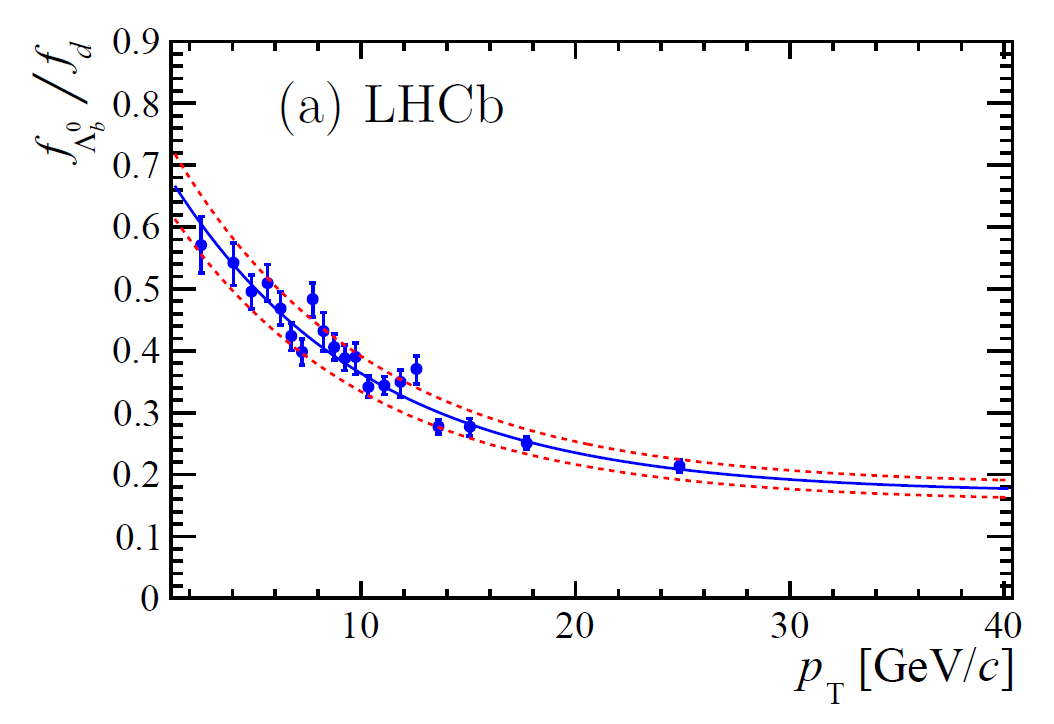
\includegraphics[width=0.49\textwidth]{Lb_production_pt_dependence}
	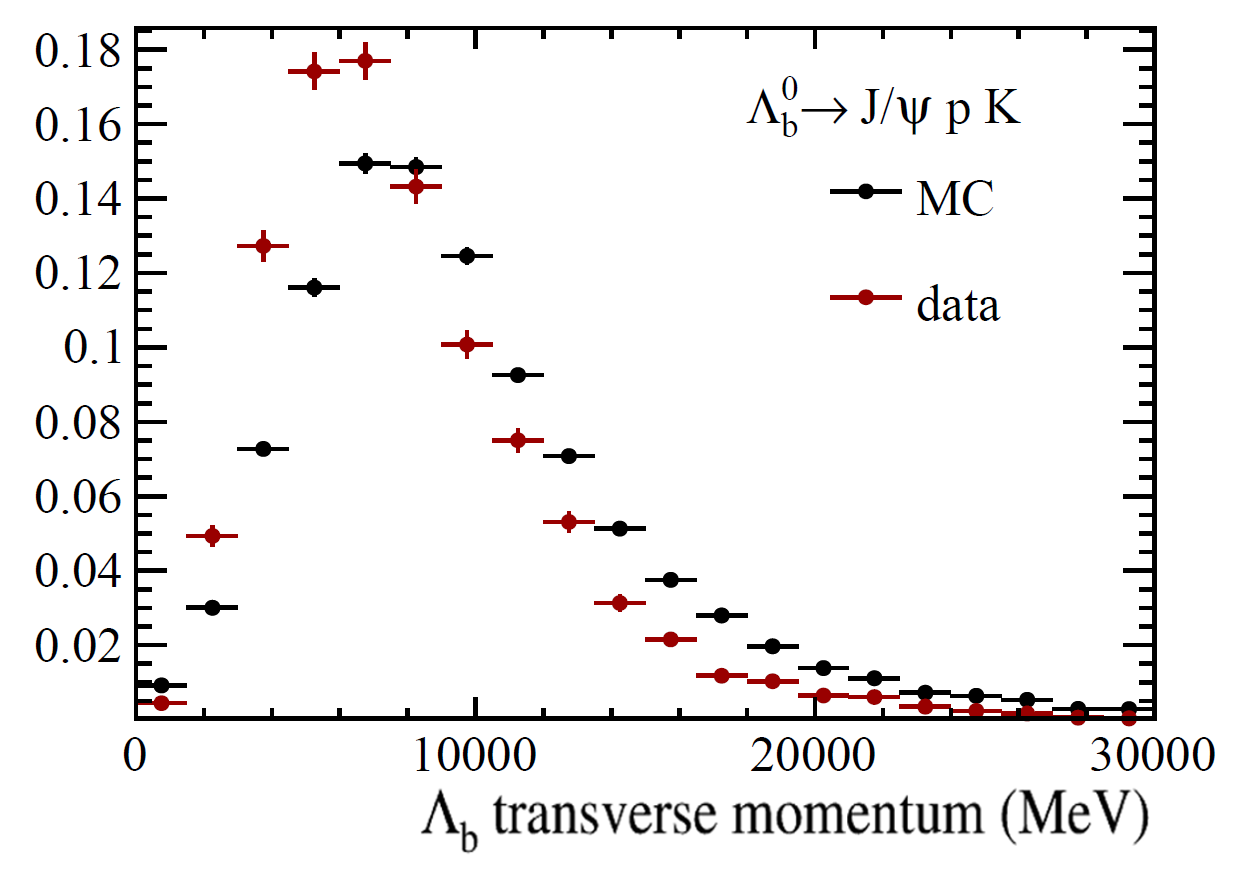
\includegraphics[width=0.49\textwidth]{Lb_pt_comparison_weights}
	\caption{Left: Ratio of \Lb to \Bd production as a function of \pt. Figure taken from \cite{Lb_production_kinematic}.  Right: Transverse \Lb momentum for \decay{\Lb}{\jpsi\Dz\proton} decays in data and simulation. Figure taken from the documentation belonging to \cite{SL_Vub}.}
	\label{fig:LbPTrew}
\end{figure}


\section{Reweighting of the \LbToDpmunuX decay simulation}
\label{sec:Reweight_D0p}
It has already been mentioned that the underlying physics in the \LbToDpmunuX simulation is wrong.
Since there aren't any theoretical predictions on that channel, the reweighting of the simulation has to be done carefully.
To come as close to data as possible, a threedimensional reweighting in the variables
\begin{itemize}
    \item M(\Dz\proton)
    \item M(\Dz\mun)
    \item M(\Dz\proton\mun)
\end{itemize}
has been chosen. 
This choice is not trivial and above all obvious, but there are several reasons for it:
\begin{enumerate}
    \item The simulation is completely off from the data distribution in these variables.
    \item These variables are already available at generator level, i.e. before the detector response is simulated. 
          To calculate the selection efficiency the simulation has to be reweighted at generator stage as well.
    \item There aren't any selection requirements on these variables. 
          Otherwise, no weights could be assigned to ones not fulfilling the requirements at generator level
          \footnote{There exists a selection requirement on M(\Dz\proton\mun) in this analysis to eliminate \decay{\Lb}{\Dz\proton\pim} background, but less than 0.5\% of all events have their generated mass above this value. 
                    Thus, its impact on the efficiency can be neglected.}.
\end{enumerate}
After the description of the reweighting and efficiency calculation process, it should become clear why these three points are important:
\begin{itemize}
    \item \textbf{Determination of the weights} \\
          There are two normalized threedimensional histograms drawn for both, generated events (in the following called MCDecayTreeTuple or MCDTT) and events after reconstruction, applying selection cuts and the kinematic reweighting (DecayTreeTuple or DTT). 
          Both histograms have the three variables mentioned above on their axes.
          The histogram with the weights is now calculated by dividing the DTT histogram through the MCDTT histogram.
    \item \textbf{Assigning weights to the events} \\
          Now, this weight histogram is used to assign a weight to each DTT (\weight{DTT}) and MCDTT (\weight{MCDTT}) event.
          To get the correct bin in the weight histogram the generated masses \Mtrue{\Dz\proton}, \Mtrue{\Dz\mun} and \Mtrue{\Dz\proton\mun} are used.
    \item \textbf{Calculation of the efficiency} \\
          The efficiency can now be calculated with
          \begin{align}
              \epsilon = \frac{\sum \weight{DTT}}{\sum \weight{MCDTT}}, \label{eq:effrew}.
          \end{align}
          To account for the loss of statistical power due to reweighting, both numerator and denominator in equation (\ref{eq:effrew}) are multiplied by the renormalisation factor $\sum \weight{MCDTT} / \sum \weight{DTT}^2$. 
          This doesn't affect the central value of $\epsilon$ but influences the statistical error, which is calculated using binomial statistics.
\end{itemize}
It should now be clear, that with this procedure one must not cut on the weighting variables, since otherwise the weights outside the cut region would be zero. 
Hence it wouldn't be clear which weights have to be assigned to the MCDTT events. 
The distribution of the masses after reweighting are also shown in figure \ref{fig:reweighting}.
A decided improvement of the data description can be figured out.
Many more comparisons between data and simulation before and after reweighting can be found in the appendix \ref{app:Reweight_D0p} in figure \ref{fig:reweight_D0p_app}.
Having these reweighting steps in mind, it is now possible to calculate the efficiencies at different stages.

Concerning the channel \LbToLcmunu no further reweighting is applied since the agreement in the comparison between data and simulation seems to be sufficient.
Several comparison plots on this channel can be found in figure \ref{fig:reweight_Lc_app} in \ref{app:Reweight_Lc}.


\section{Generator level efficiencies}
As a reminder, generator level efficiencies arise due to the fact, that one demands the generated events to be in the \lhcb acceptance and apply some (loose) requirements on the kinematics to accelerate the simulation process.
The generator level samples are reweighted as described above: the \LbToLcmunu sample with the kinematic \pt(\Lb) reweighting and the \LbToDpmunu sample with both reweightings.
For signal and normalization channel the following generator level efficiencies are obtained:
\begin{align*}
    \effGenLc &= \effGenLcval \pm \effGenLcerr, \\
    \effGenDp &= \effGenDpval \pm \effGenDperr.
\end{align*}

\section{Reconstruction and selection efficiencies}
The reconstruction and selection efficiencies are calculated analogously.
The same reweighting procedure on the different samples is performed.
The results for signal and normalization channel are:
\begin{align*}
    \effSelLc &= \num[scientific-notation=true]{\effSelLcval \pm \effSelLcerr}, \\
    \effSelDp &= \num[scientific-notation=true]{\effSelDpval \pm \effSelDperr}.
\end{align*}

\section{Total efficiencies}
To summarise the values above the total efficiencies for the channels are:
\begin{align*}
    \effDp &= \effGenDp \cdot \effSelDp = \num[scientific-notation=true]{\effDpval \pm \effDperr}, \\
    \effLc &= \effGenLc \cdot \effSelLc = \num[scientific-notation=true]{\effLcval \pm \effLcerr}.
\end{align*}
For the consideration of systematics later it is sometimes more useful to consider the ratio of both efficiencies
\begin{align*}
    \frac{\effLc}{\effDp} = \effRatioval \pm \effRatioerr.
\end{align*}

	%\chapter{Backgrounds}
\label{sec:Backgrounds}

The big disadvantage of semileptonic decays is that the neutrino can't be reconstructed.
At hadron colliders like the \lhc is it impossible to know the initial state, so one doesn't have enough constraints to reconstruct the full kinematic information about the decaying particle.
Being aware of these problems due to experimental setup it is clear that one can't use a well reconstructed \Lb mass peak to separate signal from background.
A main source of background is expected to be the decay \decay{\Bd/\Bp}{\Dz\mun\neumb X} where one randomly combines a proton to this decay.
Ths background is handled by the fit of the \logIP distribution.
Other sources of backgrounds and their possible impact on the obtained signal yield \NDp are discussed in the following.
For the \LbToLcmunu channel it is assumed, that all non-negligible backgrounds are accounted for due to the sidebandsubtraction and including wrong sign events as well as resonant modes components in the fit.
The discussion in this chapter thus refers completely to the \LbToDpmunuX channel.

% ====================================
% section: proton misidentification
% ====================================
\section{Proton misidentification}
A possible source of backgrounds is that one misinterprets a decay as \LbToDpmunuX since one misidentifies a final state particle.
In this analysis it is most likely that the proton is misidentified since the final state pion and kaon are reconstructed to a \Dz yielding in a nice peak and the muon leaves a clear signature in the detector due to its relatively long lifetime and low interaction with matter.
Examples for these kind of backgrounds are the decays \decay{\Bs}{\Dz\Kp\mun\neumb X} and \decay{\Bd/\Bp}{\Dz\pip\mun\neumb X}, where either the \Kp or \pip is misidentified as proton.
Though there are tight requirements on the proton identification at selection stage, the data will still be polluted by misidentified particles.
To identify the amount of misidentified protons, a slightly different data sample than the nominal one is used. 
In this sample no requirements on the proton idenfication are applied.
Except for those all other requirements are the same as described in section \ref{sec:Selection}.
However the removal of the particle identification requirements lets the data size of the sample rapidly increase.
To keep the data size acceptable a so called 5\% prescaling has been applied, i.e. only 5\% of all events are actually stored.
The decision if a particle is stored or not is made by random.
That's why absolute numbers quoted in this section can't be compared to the obtained signal yields etc. in the previous sections.
The study on misidentified backgrounds is done in three steps.

\subsection{Definition of particle identification regions - Number of particle candidates}
\label{sec:PIDCalib_Ncand}
As a first step it has to be defined what requirements have to e fulfilled, that a particle is called a proton, pion or kaon.
Therefore the PID (for Particle IDentification) variables are used.
Remember, that \lhcb's particle idenitfication system provides likelihoods for each particle hypothesis.
The PID variables now describe differences between the logarithms of these likelihoods, e.g. PIDp is defined as the difference of the logarithmic likelhoods between the proton and pion hypothesis.
A value of PIDp$>0$ hence means, that the particle is more likely a proton than a pion.
Respectively, the PIDK compares kaon to pion hypothesis.
If one wants to separate protons from kaons it is useful to look at PIDp$-$PIDK.
The definition what will be called proton is motivated by the requirements applied in the analysis (see section \ref{sec:Selection}). 
In detail the regions for the identification of protons, pions and kaons are:
\begin{itemize}
\item proton: $\text{PIDp} - \text{PIDK} > 10.0 \text{ and } \text{PIDp} > 10.0$
\item pion: $\text{PIDp} < 10.0 \text{ and } \text{PIDK} < 0.0$
\item kaon: $\text{PIDp} - \text{PIDK} < 10.0 \text{ and } \text{PIDK} > 0.0$
\end{itemize}

Furthermore these regions and their population are visualised in figure \ref{fig:PIDregions}. 
From this the number of candidates for each particle species is obtained, in the following denoted as \Ncand{i}, with $i \in \left[\pi, \kaon, \proton\right]$. 
The number of candidates are
\begin{align}
    \Ncand{\pi}     &= \PIDNcandpionval \pm \PIDNcandpionerr, \\ 
    \Ncand{\kaon}   &= \PIDNcandkaonval \pm \PIDNcandkaonerr, \\ 
    \Ncand{\proton} &= \PIDNcandprotonval \pm \PIDNcandprotonerr.
\end{align}
\begin{figure}[hptb]
	\centering
	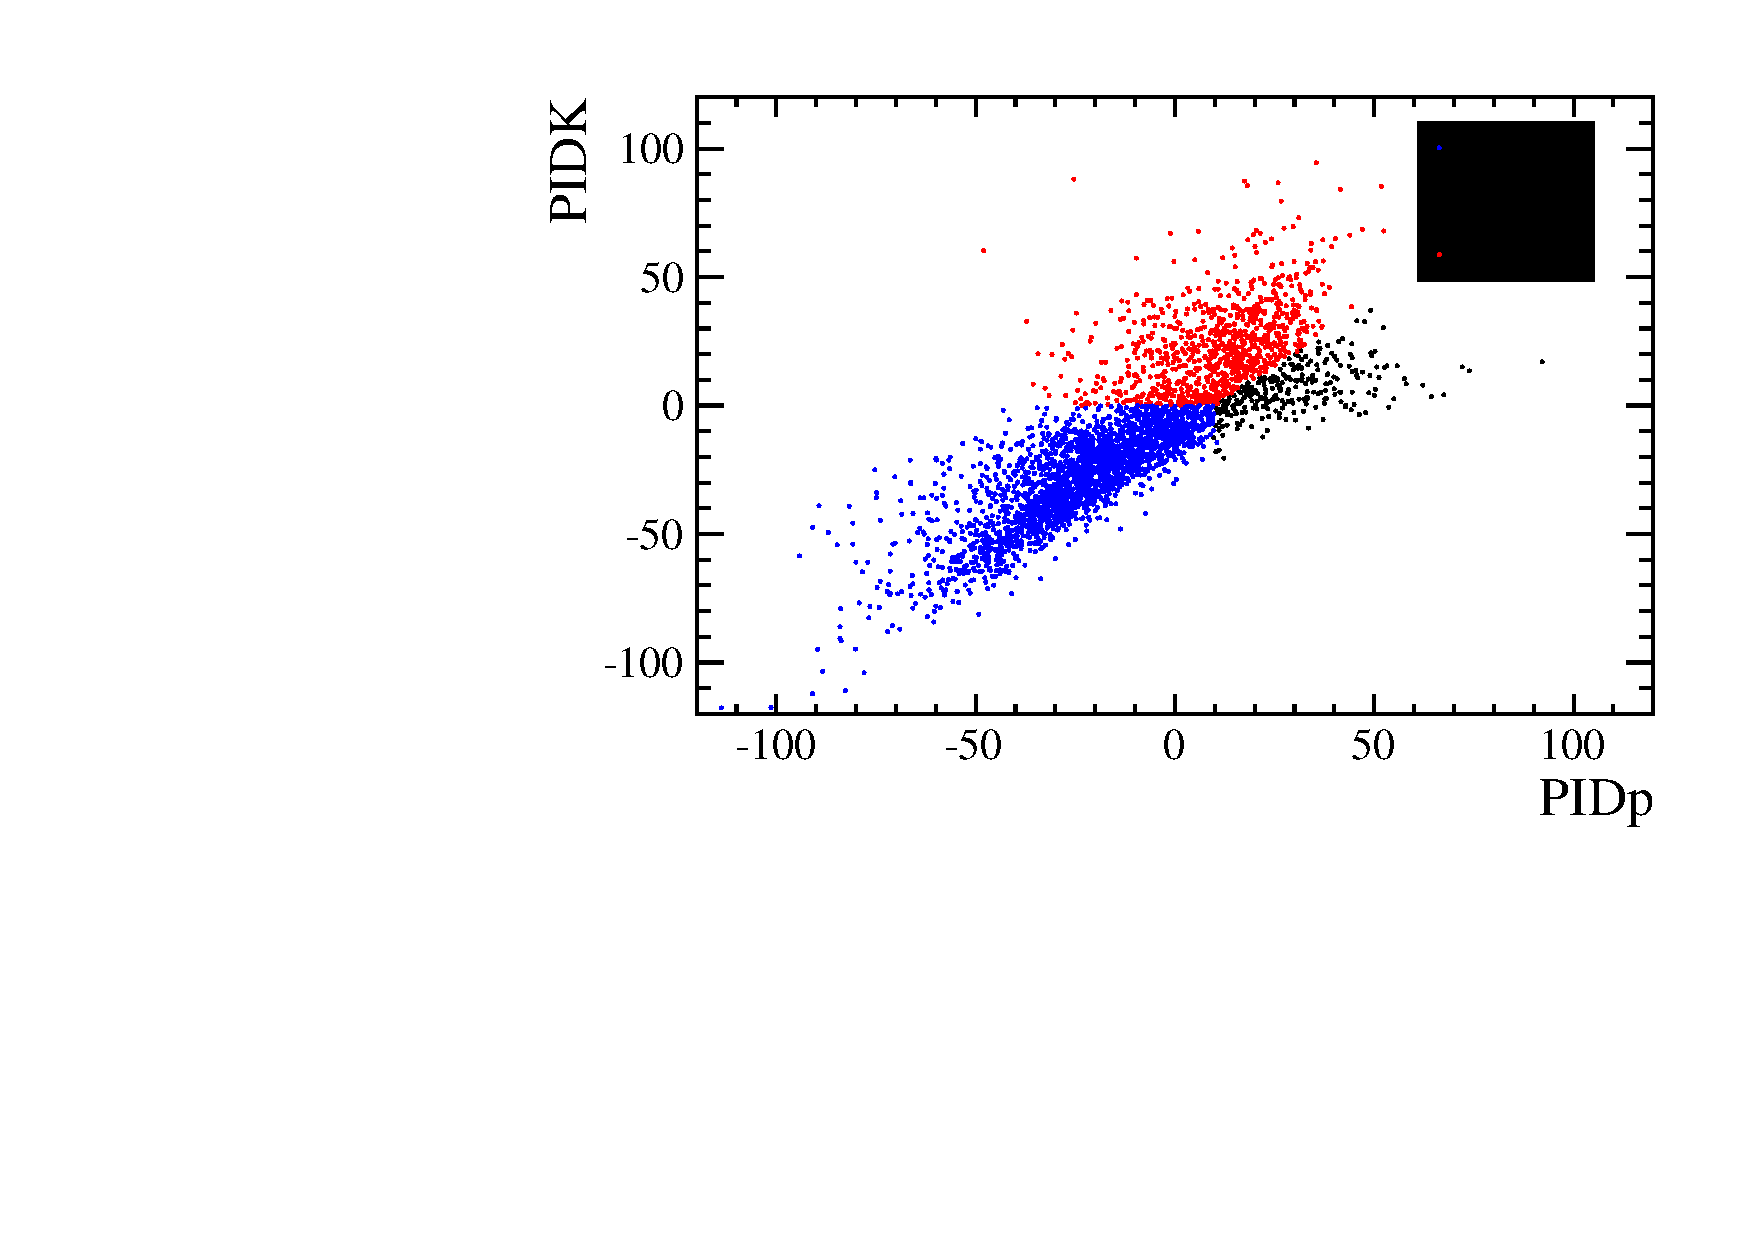
\includegraphics[width=0.49\textwidth]{LbToD0p/PID/PIDK_vs_PIDp}
	\caption{Defined regions for the number of particle candidates.}
	\label{fig:PIDregions}
\end{figure}


\subsection{Determination of ``true" candidates with PID efficiencies}
Of course, this choice of regions is a bit arbitrary and it doesn't prevent real protons, pions and kaons to enter the other regions.
With the PID variables it is only possible to increase or decrease the probability, that a particle enters a ``foreign" region.
Thus, one needs to determine the efficiencies that a real proton, pion or kaon passes the requirements for the identification of being a proton, kaon or pion.
For this purpose the \lhcb PIDcalib tool is used.
This tool includes calibration samples of decays cleanly reconstructed without use of the PID variables for instance the decay \decay{\Lambda}{\proton\pim} for the proton efficiencies.
Since no requirement on the PID has been applied before, it is now possible to study the impact of these requirements.
The PID efficiency for each of the 9 possible combinations (real particle to be identified as other particle according to PID) is determined binwise depending on the particle momentum. 
The results can be seen in figure \ref{fig:PIDefficiencies}.
\begin{figure}[hptb]
	\centering
	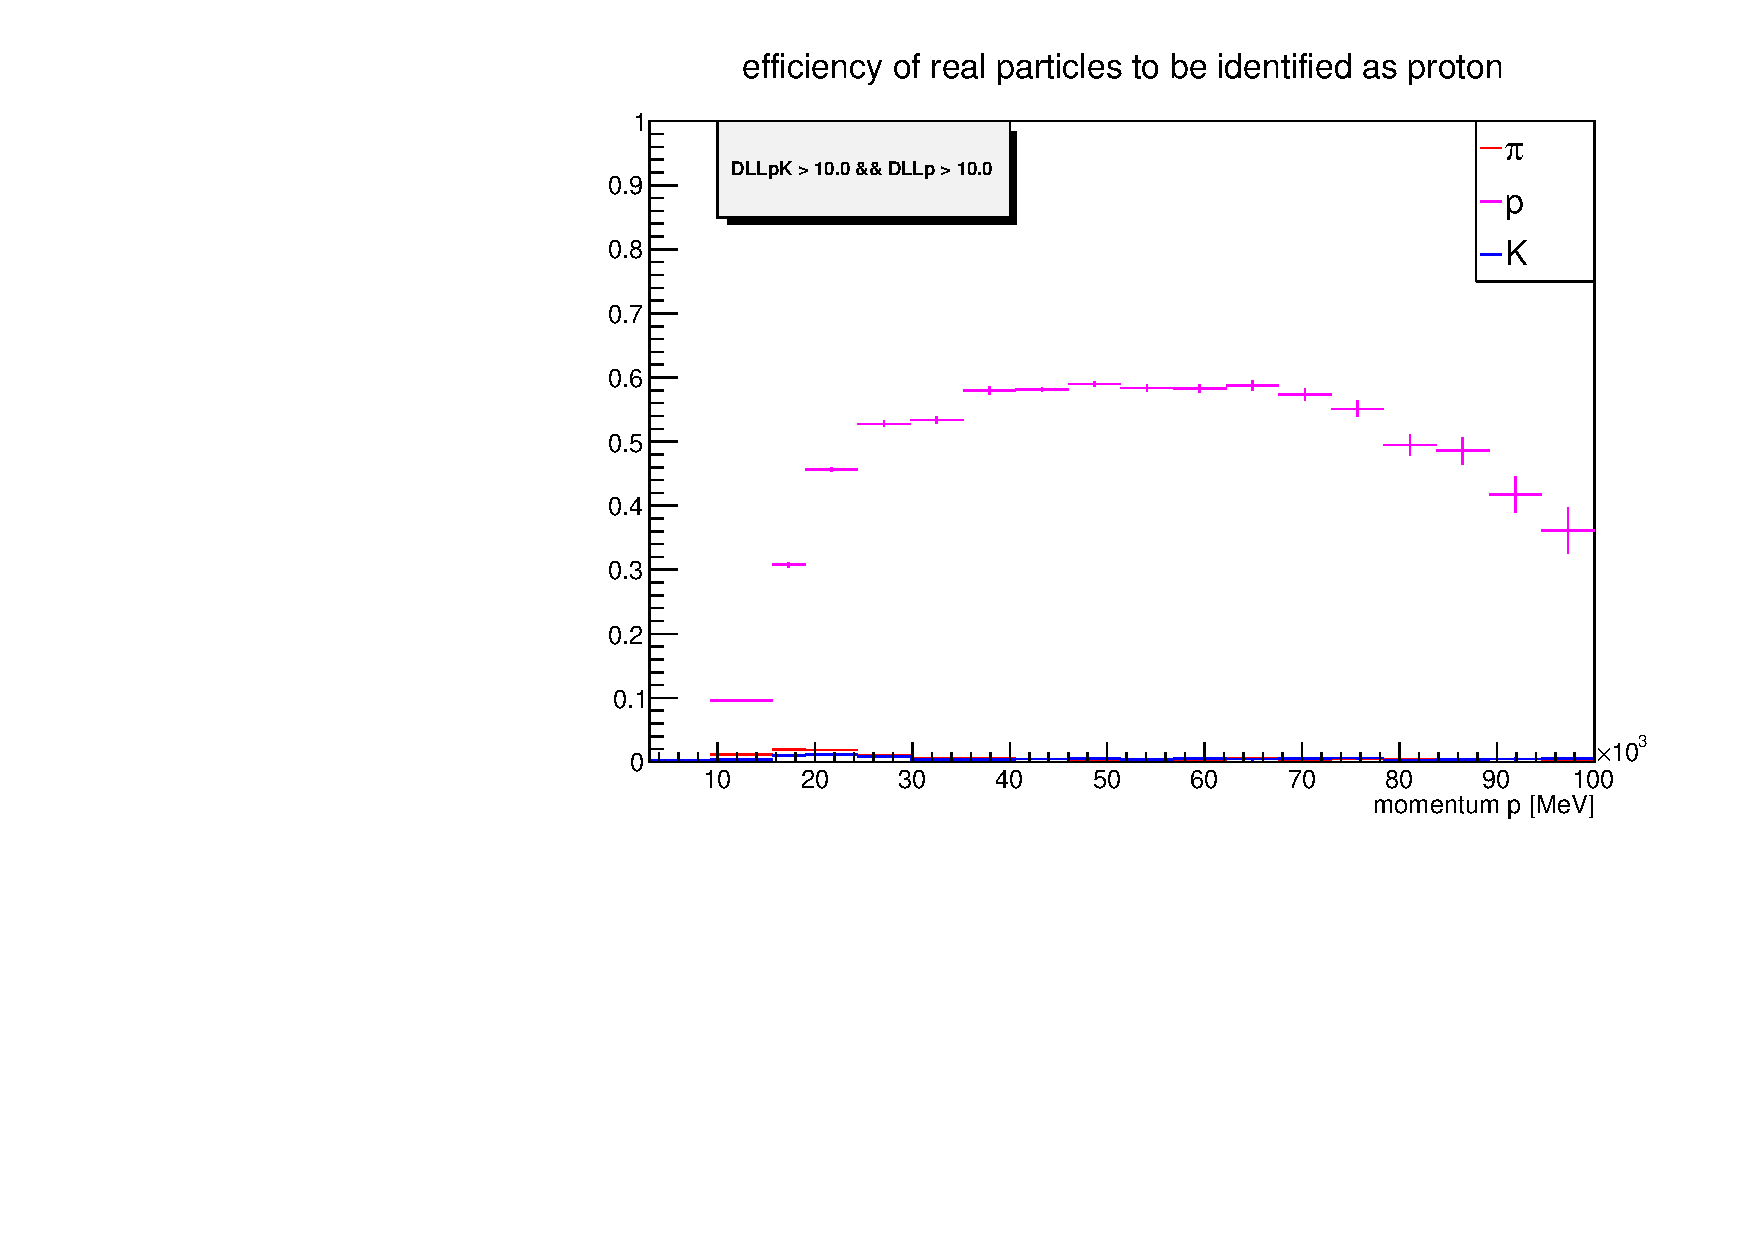
\includegraphics[width=0.32\textwidth]{LbToD0p/PID/PID_proton}
	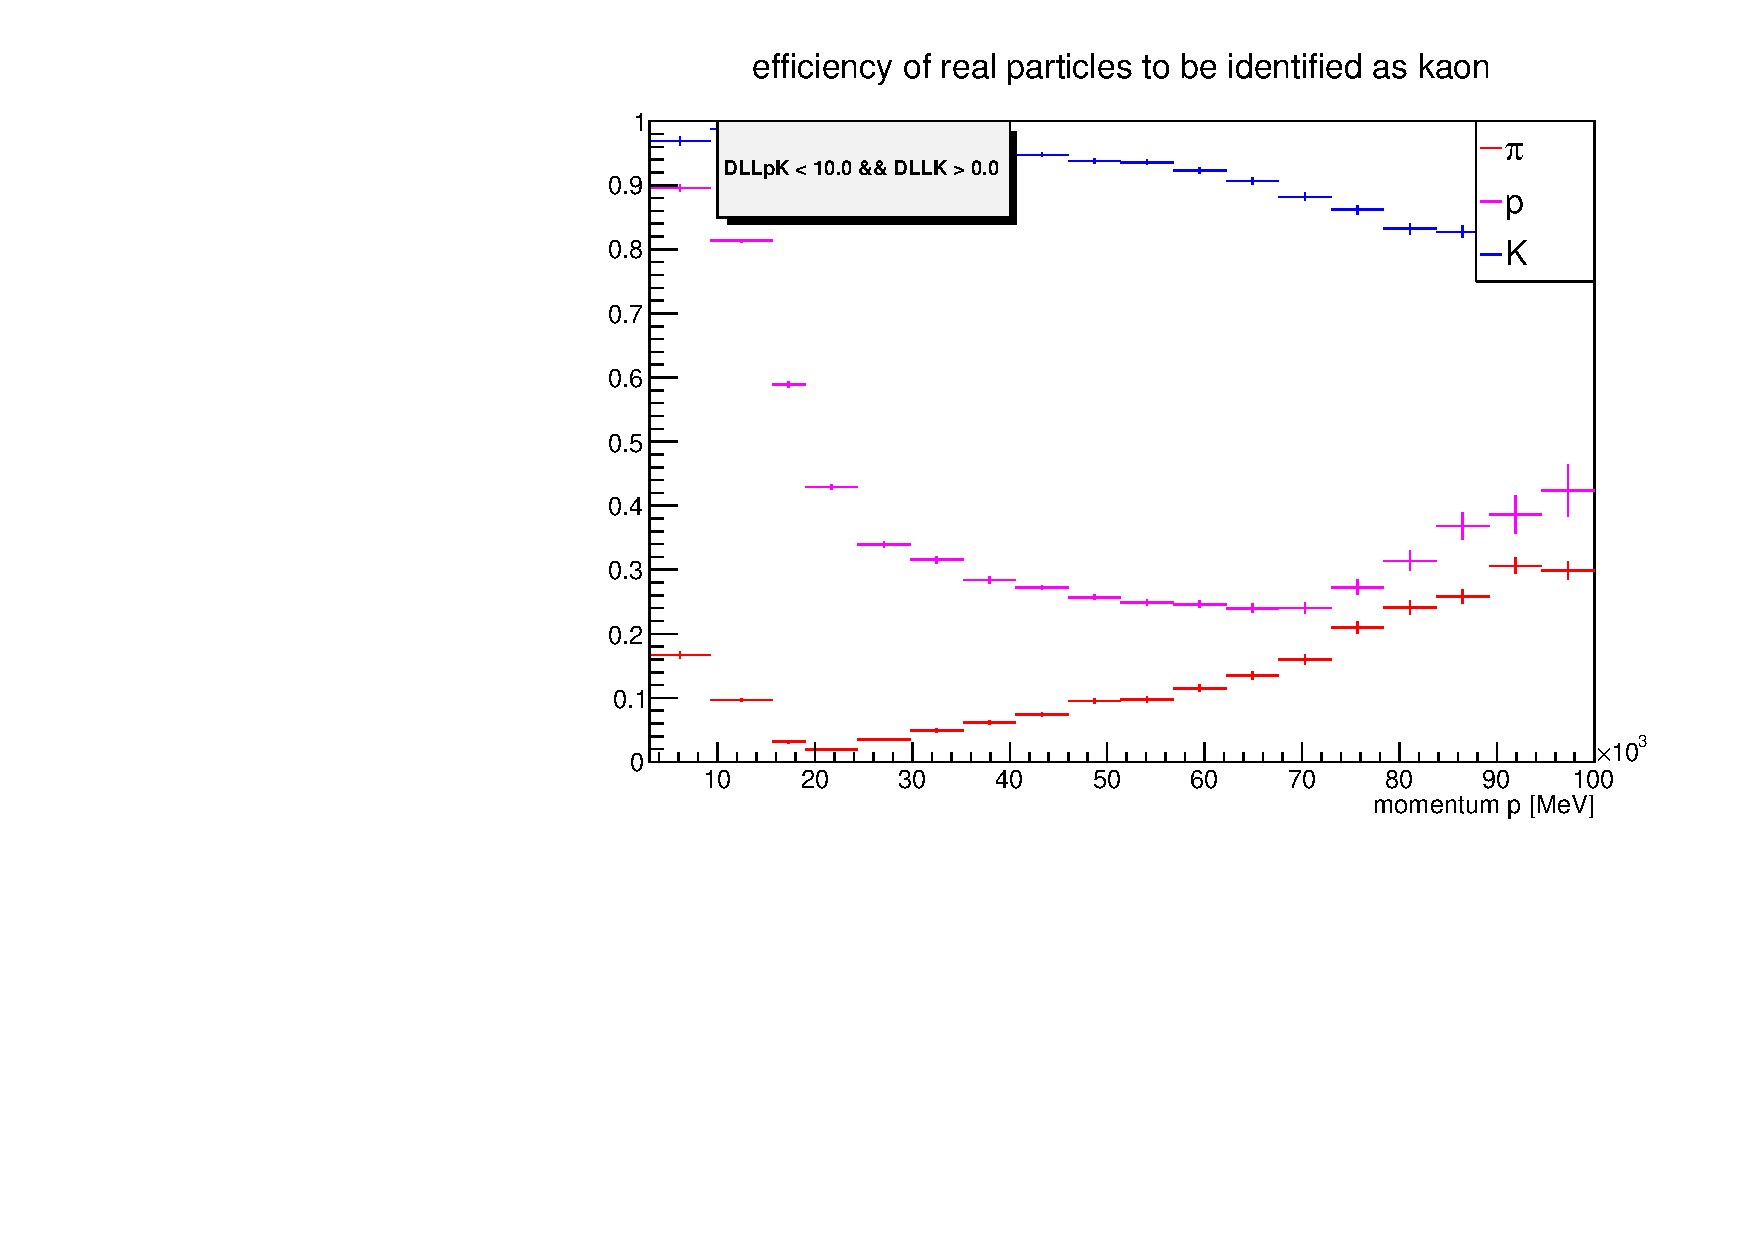
\includegraphics[width=0.32\textwidth]{LbToD0p/PID/PID_kaon}
	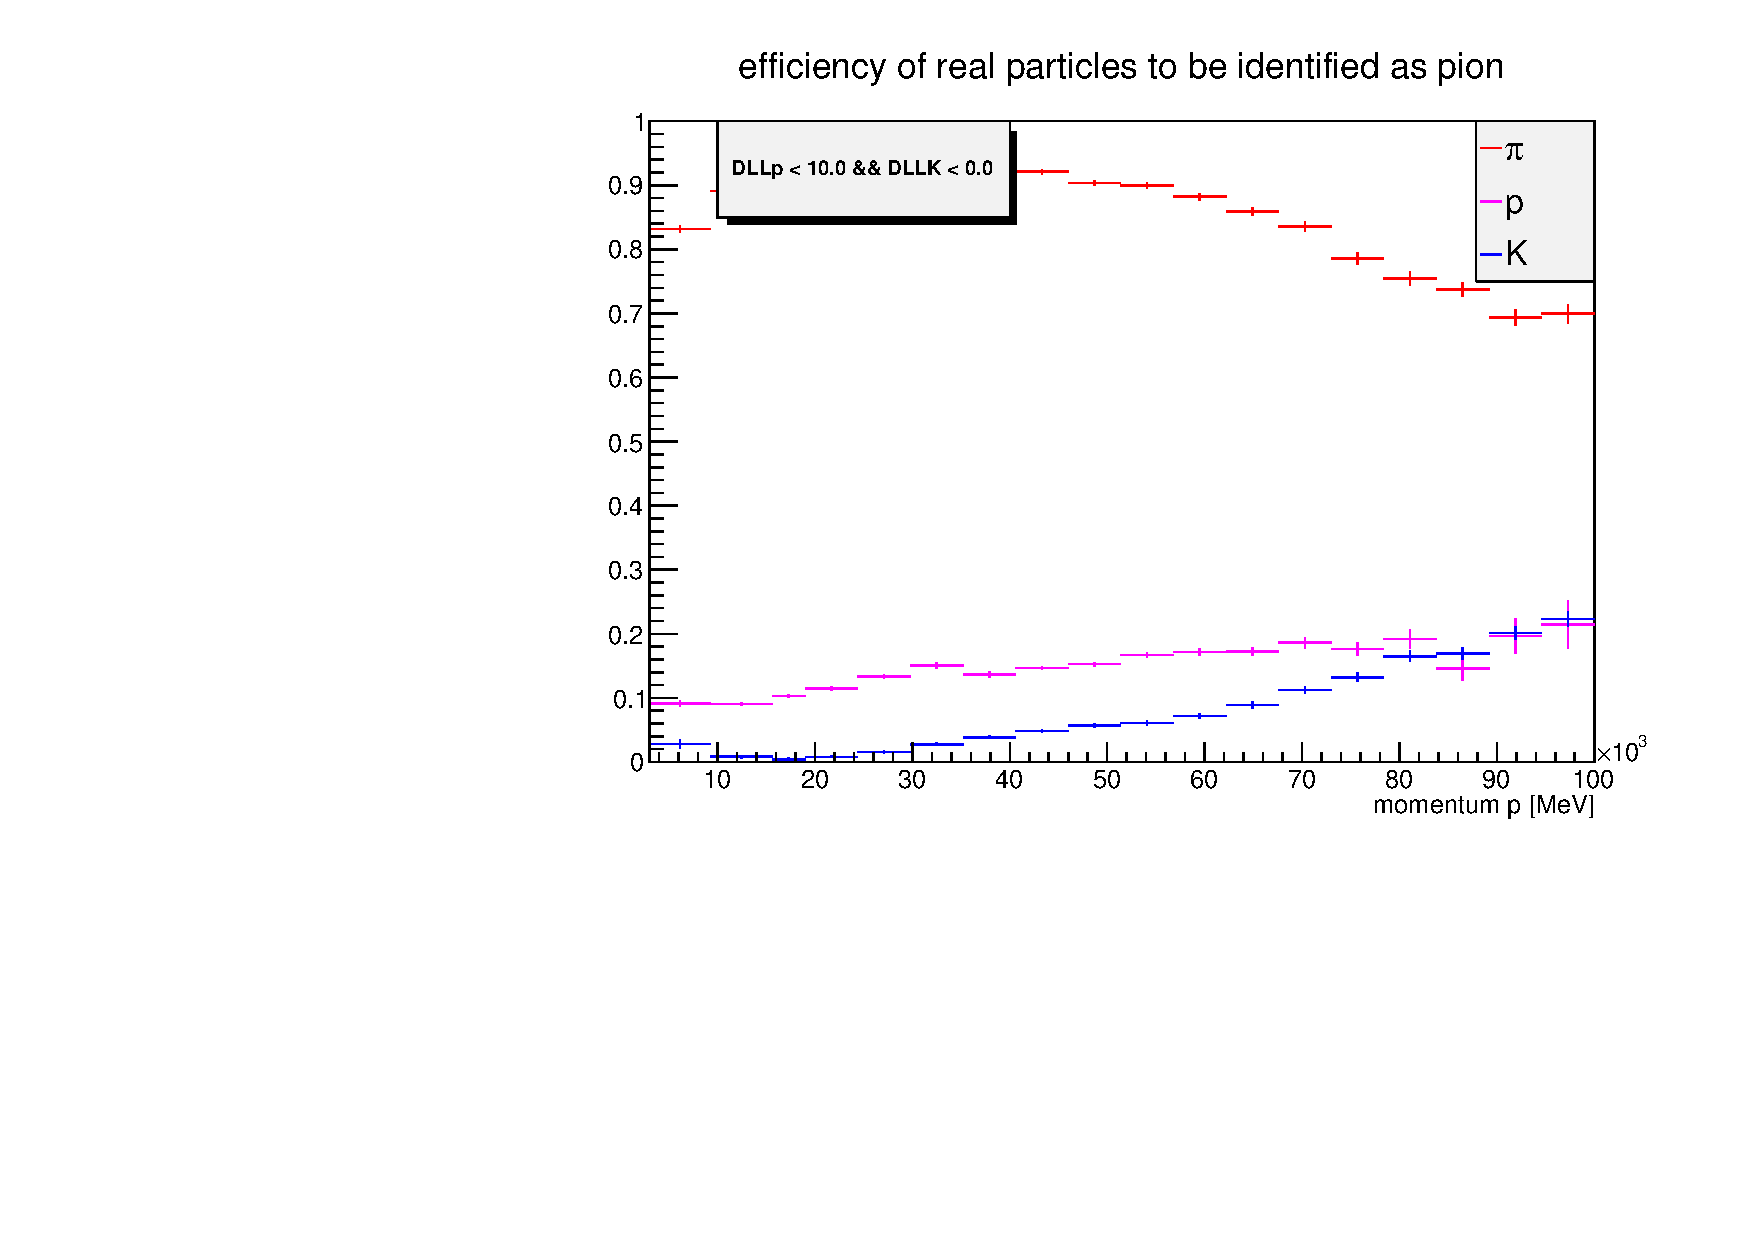
\includegraphics[width=0.32\textwidth]{LbToD0p/PID/PID_pion}
	\caption{Efficiencies that real protons, kaons and pions are identified as protons (left), kaons (middle) or pions (right). The tight requirements on the proton PID applied in this analysis ensures that only few kaons and pions enter the proton region paying the prize, that one looses a lot of
    protons as well.}
	\label{fig:PIDefficiencies}
\end{figure}
To determine a final value for each efficiency, these histograms are weighted with respect to the kinematic distribution of this analysis' data sample. 
The result is:
\begin{align*}        
\begin{pmatrix}
    \effPID{\pip}{\pip}    & \effPID{\Km}{\pip}    & \effPID{\proton}{\pip} \\
    \effPID{\pip}{\Km}     & \effPID{\Km}{\Km}     & \effPID{\proton}{\Km} \\
    \effPID{\pip}{\proton} & \effPID{\Km}{\proton} & \effPID{\proton}{\proton} 
\end{pmatrix}
=
\begin{pmatrix}
0.9409 & 0.0241 & 0.1309 \\
 0.0474 & 0.9681 & 0.3798 \\
 0.0117 & 0.0077 & 0.4893
\end{pmatrix}
\end{align*}

Here, \effPID{i}{j} denotes the efficiency, that a real (true) particle $i$ is identified as what is call $j$ according to the particle regions defined in section \ref{sec:PIDCalib_Ncand}. 
For the following steps, PID efficiency errors are assumed to be negligible compared to the corresponding uncertainties of the particle candidates \Ncand{i}.
With the PID efficiencies \effPID{i}{j} and the number of particle candidates \Ncand{k}, the number of real (true) particles can now be estimated by solving the matrix equation
\begin{align*}
    \begin{pmatrix} 
        \Ncand{\pi} \\ \Ncand{\kaon} \\ \Ncand{\proton}
    \end{pmatrix}
    =
    \begin{pmatrix}
       \effPID{\pi}{\pi}     & \effPID{\kaon}{\pi}     & \effPID{\proton}{\pi} \\
       \effPID{\pi}{\kaon}   & \effPID{\kaon}{\kaon}   & \effPID{\proton}{\kaon} \\
       \effPID{\pi}{\proton} & \effPID{\kaon}{\proton} & \effPID{\proton}{\proton} 
    \end{pmatrix}
    \begin{pmatrix} 
        \Ntrue{\pi} \\ \Ntrue{\kaon} \\ \Ntrue{\proton }
    \end{pmatrix},
\end{align*}
which delivers
\begin{align}
    \Ntrue{\pi}     &= \PIDNtruepionval \pm \PIDNtruepionerr, \\ 
    \Ntrue{\kaon}   &= \PIDNtruekaonval \pm \PIDNtruekaonerr, \\ 
    \Ntrue{\proton} &= \PIDNtrueprotonval \pm \PIDNtrueprotonerr.
\end{align}
\Ntrue{i} denotes the number of real particles $i$ in the sample.

\subsection{Estimate of misidentified protons}
Using the results of the previous subsections it is now possible to estimate the number of misidentified protons, i.e.``true" kaons or pions entering the proton region.
This is calculated by multiplying the number of ``true" particles \Ntrue{i} with the PID efficiency \effPID{i}{\proton} to be identified as proton. 
\begin{align}
    N^{\pi}     &= \effPID{\pi}{\proton} \Ntrue{\pi}         = \PIDNtruePregionpionval \pm \PIDNtruePregionpionerr, \\  
    N^{\kaon}   &= \effPID{\kaon}{\proton} \Ntrue{\kaon}     = \PIDNtruePregionkaonval \pm \PIDNtruePregionkaonerr, \\ 
    N^{\proton} &= \effPID{\proton}{\proton} \Ntrue{\proton} = \PIDNtruePregionprotonval \pm \PIDNtruePregionprotonerr.
\end{align}
Thus, the amount of misidentified protons is at a single-digit percent level, namely $(\misIDratioval \pm \misIDratioerr)\%$. 
Note again, that the absolute values can't be compared to the signal yields obtained in previous parts of this analysis.
It is only the lastly quoted ratio which can be used in the following.

\section{Misidentified muons}
Though not as prominent as misidentified protons, the misidentification of muons is also considered.
One possibility is that the muon is misidentified from an exclusive 3 body decay of the \Lb for instance \decay{\Lb}{\Dz\proton\pim}.
If this is the case, the decay isn't semileptonic but rather hadronic.
Consequently, the \Lb can be fully reconstructed since all final state particles are seen.
This should lead to a peak in the invariant \Dz\proton\mun around the \Lb mass.
There's indeed such a peak as figure \ref{fig:plot_D0pmuMass} shows.
These kind of backgrounds can thus easily eliminated by vetoing \Dz\proton\muon masses around the \Lb mass, in this case all masses above 5500\mev.
\begin{figure}[hptb]
	\centering
	\includegraphics[width=0.49\textwidth]{LbToD0p/plots/data/Bh_M}
	\caption{Invariant \Dz\proton\mun mass. A peak at \Lb mass ($\approx 5620 \mev$) can be seen caused by misidentified muons coming from hadronic decays like \decay{\Lb}{\Dz\proton\pi} where the pion is misidentified as muon. 
             A veto on the \Dz\proton\mun mass indicated by the arrow eliminates such backgrounds.}
	\label{fig:plot_D0pmuMass}
\end{figure}

The situation becomes more tricky, if the background is coming from a more body \Lb decay, i.e. a decay with more than 3 final state particles.
Since this analysis aims to measure the inclusive branching ratio \BR(\LbToDpmunuX), misidentified muons could also come from decays like \decay{\Lb}{\Dz\proton 3\pi}, where one of the 3 pions is misidentified as muon.
These backgrounds aren't easy to eliminate, since the other 2 pions aren't reconstructed and thus not peaking in \Dz\proton\mun mass.
Nonetheless if they're existent in the data sample it might be possible, that such backgrounds tend to sit at lower PIDmu of the muon saying the lower the PIDmu of a muon is the more likely it is to be a misidentified particle.
Unfortunately no distinct structures can be seen in figure \ref{fig:plot_D0pmuMass_vs_muPIDmu}.
This might be a hint that these backgrounds play a minor role.
Assuming that the decay \decay{\Lb}{\Dz\proton 3\pi} behaves in comparison to \decay{\Lb}{\Dz\proton\pim} similar to the Meson decays \decay{\Bd}{\Dm 3\pi} and \decay{\Bd}{\Dm\pip} with 
$\BR(\decay{\Bd}{\Dm 3\pi}) = (2.76 \pm 0.13) \cdot 10^{-3} \approx$ 
$\BR(\decay{\Bd}{\Dm\pip}) = (2.68 \pm 0.13) \cdot 10^{-3}$ (see \cite{PDG})
they should have similar branching ratios and thus should equally leak as background into this analysis.
A comparison with $\BR(\decay{\Bd}{\Dm 3\pi})/\BR(\decay{\Bd}{\Dm\ellp\neul}) \approx 10\%$ and the misidentification probabilty of a hadron of less than $10\%$ \cite{muonID_Performance} justifies the assumption that this background leaks with about $1\%$ in the signal yield.
To account for other possible but not yet measured peaking backgrounds such as \decay{\Lb}{\Dz\proton\rhom}, \decay{\Lb}{\Dz\proton\pim\rhoz} and so on a total peaking background ratio of $(5.0 \pm 2.5)\%$ is assumed.
\begin{figure}[hptb]
	\centering
	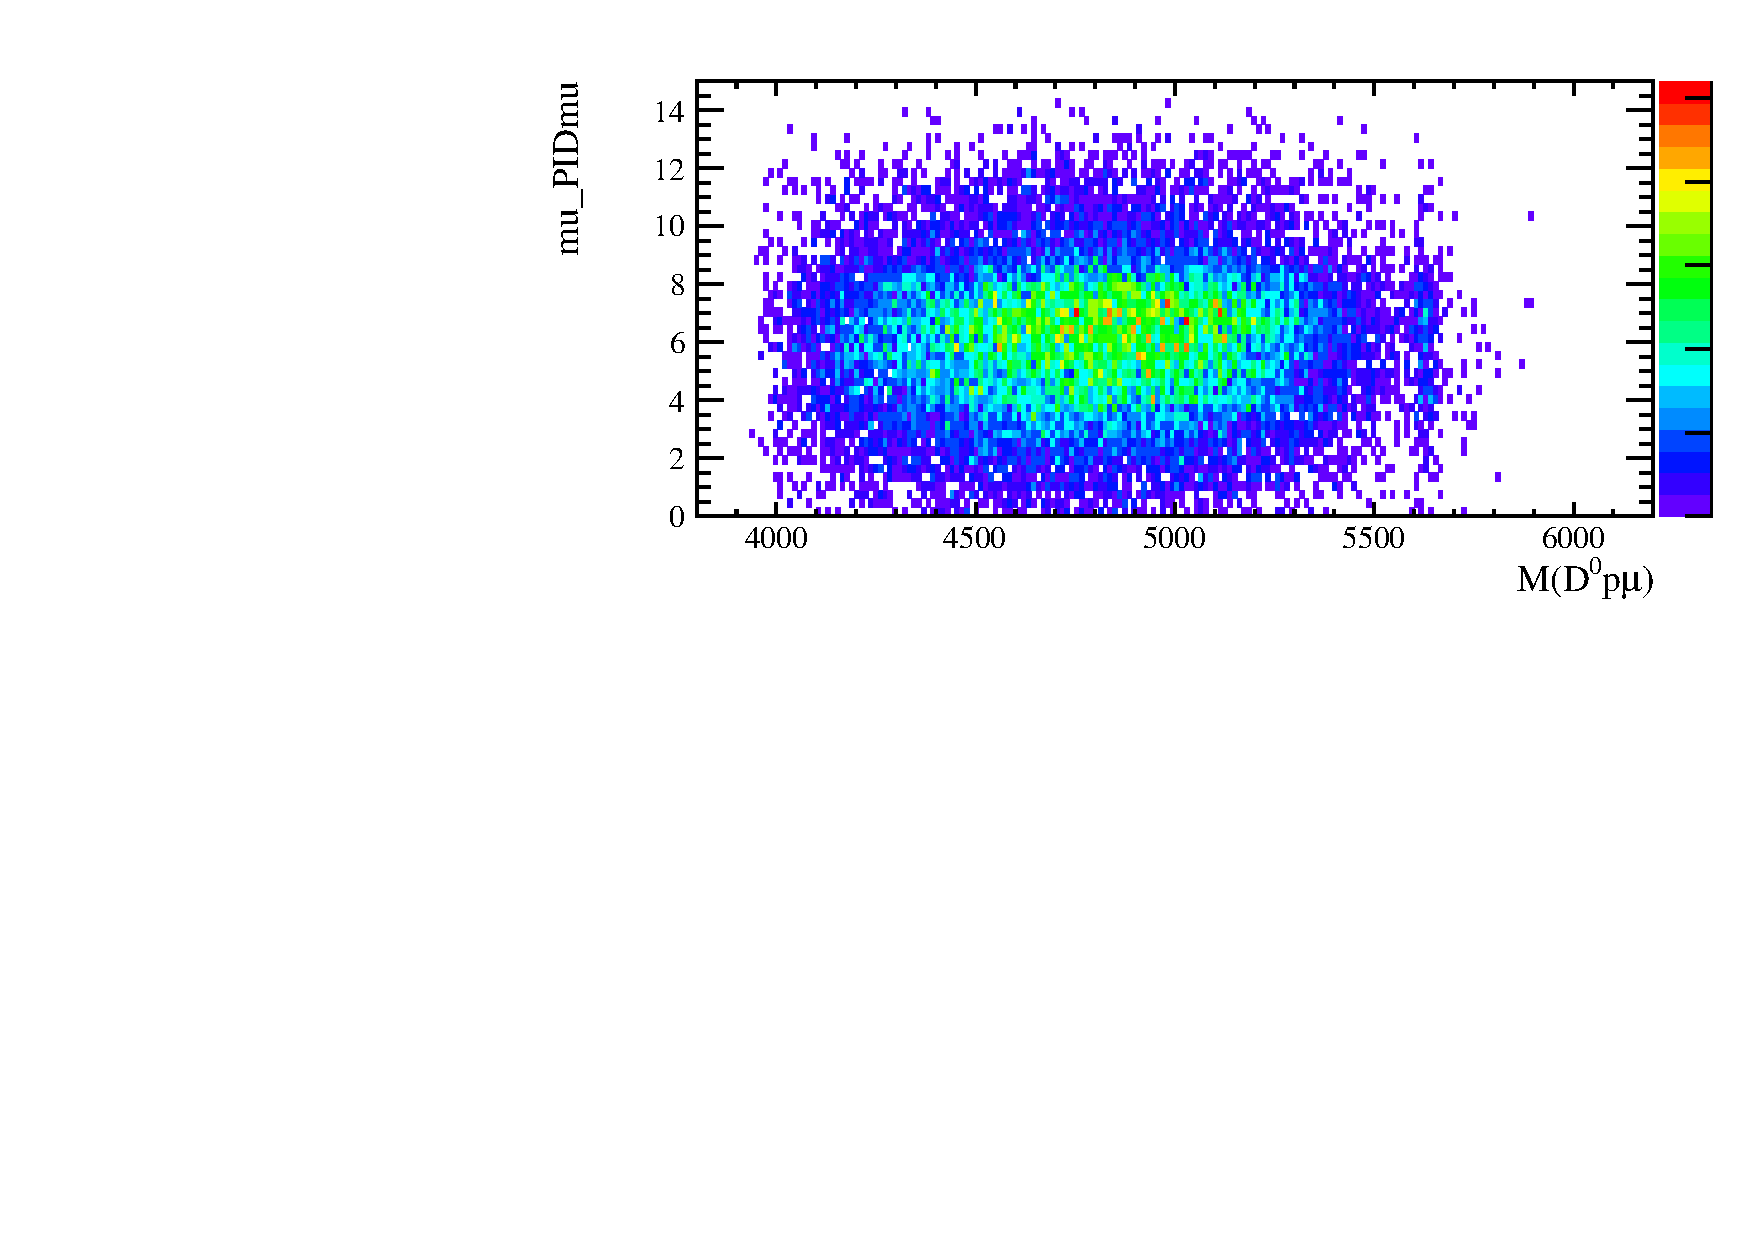
\includegraphics[width=0.49\textwidth]{LbToD0p/plots/data/Bh_M_vs_mu_PIDmu_RS}
	\caption{Invariant \Dz\proton\mun mass versus PIDmu of the muon. No structures tending to low PIDmu can be seen.}
	\label{fig:plot_D0pmuMass_vs_muPIDmu}
\end{figure}

\section{Prompt \Dz}
With prompt \Dz one denotes \Dz coming directly from the primary \proton\proton interaction being not a product of other decaying particles.
The production of prompt charm and hence prompt \Dz is usually a lot higher than the production of \Lb baryons. 
One typically measures a ``few" percent prompt charm background in semileptonic \bquark-hadron decays.
As crosscheck the logarithm of the \Dz impact parameter with respect to the primary vertex is plotted.
Prompt \Dz should have a smaller impact parameter compared to \Dz coming from the \Lb decay.
This should become more clearly visible in wrong sign combinations.
With a view to figure \ref{fig:plot_D0_IP} no discrepancies between data and different wrong sign combinations can bee seen which would indicate the influence of prompt \Dz backgrounds.
Compared to other background sources this kind of background seems to be negligible having furthermore in mind that there are additional cuts applied to combine the \Dz with the other particles to form a \Lb candidate.
\begin{figure}[hptb]
	\centering
	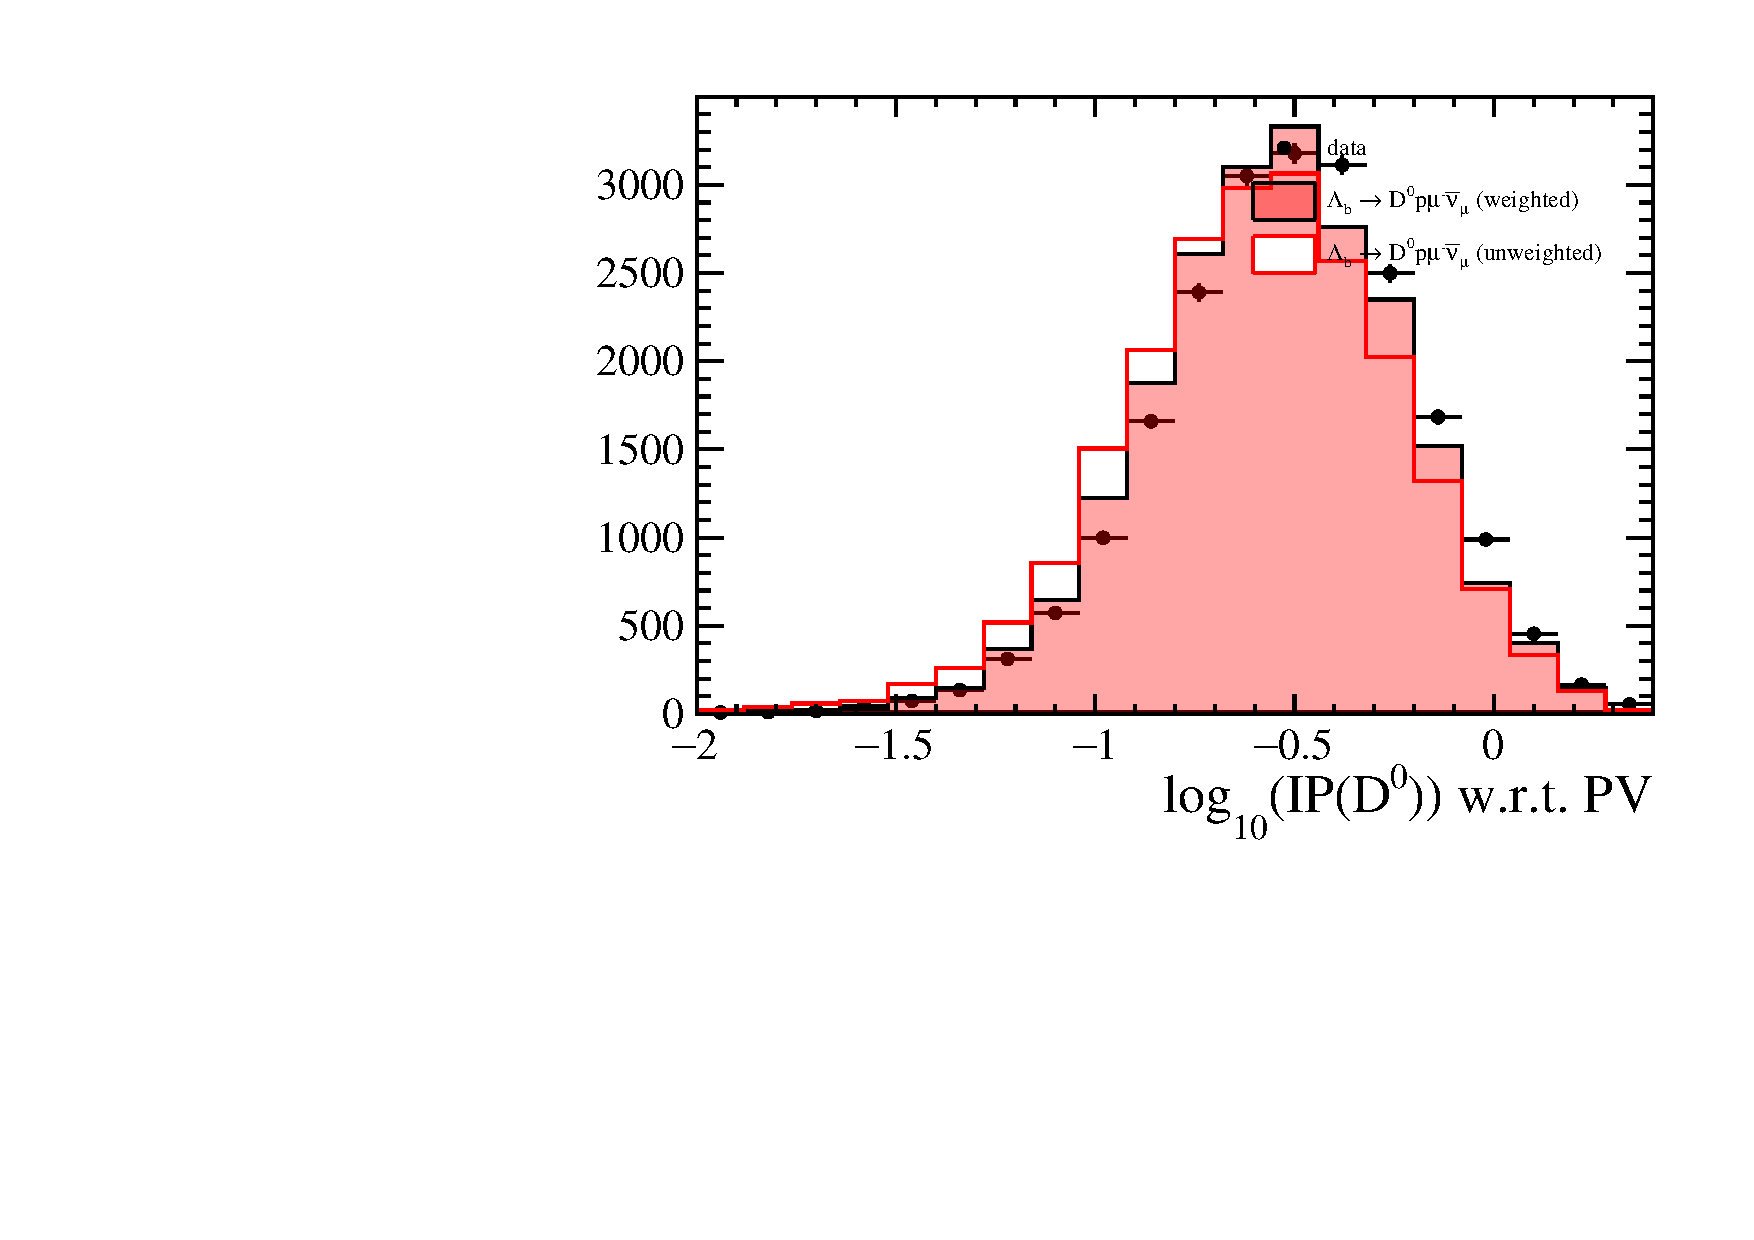
\includegraphics[width=0.49\textwidth]{LbToD0p/plots/data/D0_IP_OWNPV}
	\caption{Logarithm of the \Dz impact parameter with respect to the primary \proton\proton interaction. No special behaviour indicating prompt \Dz background can be seen.}
	\label{fig:plot_D0_IP}
\end{figure}

\section{Other possible backgrounds}
In this section some possible backgrounds not being studied in this analysis are mentioned.
Some of the decays mentioned here haven't been measured or seen so far but should be possible.
\begin{itemize}
    \item $\Lambda_b^0 \rightarrow \Dm \Lc$ \\
          This decay hasn't been measured but it should have a branching ratio of around $10^{-2}$, similar to $B \rightarrow D D_s$.
          If the \Lc decays to \pKpi, there should be another $4 \times 10^{-2}$ and in addition one needs to get the muon from somewhere else, or it has to be from $\Km \rightarrow \mun$ misidentifaction. 
          The vertex quality will be spoilt by the \Lc flight.
          Taking all these arguments together, this should be a sub-percent-level background and thus negligible in this study.
    \item $\Lambda_b^0 \rightarrow D^0 D^- p$ \\
          This decay hasn't been measured but it should be similar to $B \rightarrow DDK$ at a few times $10^{-3}$.
          The inclusive $\Dm \rightarrow \mun X$ branching fraction is about $10^{-2}$.
          So this might be still a percent level background.
    \item prompt \LcResI or \LcResII decays with a \mun from somewhere else \\
          This background should be reduced by requiring the \LcResI resp. \LcResII vertex to be well separated from the PV as done by the combination with a muon to make a \Lb candidate.
    \item \decay{\SigmabRes}{\Lb \pi}, \\ 
          where the pion isn't reconstructed.
          The knowledge about \SigmabRes is very poor.
          The production of \SigmabRes compared to \Lb should be much smaller.
\end{itemize}

\section{Backgrounds summary and estimate of background yield}
The largest background contributions leaking into the signal yield \NDp obtained by the twodimensional fit are discussed to come from either misidentified protons or muons.
All other backgrounds seems to be negligible compared to the latter ones.
Adding them up leads to a total ratio of background events in the signal yield of $(\NDpBKGratioval \pm \NDpBKGratioerr)\%$.
This corresponds to a number of background events of 
\begin{align*}
    \NBgdDp = \NDpBKGval \pm \NDpBKGerr.
\end{align*}
Note that the error on the background ratio goes into the systematic uncertainties.

	%\chapter{Systematics}
\label{sec:Systematics}
In this section studies on systematic uncertainties are presented.
They will not be presented as systematic uncertainty on \R, but rather discussed separately for the signal yields and the efficiencies.

\section{Branching ratio uncertainty of subsequent decays}
Regarding equation (\ref{eq:R}) a precise knowledge of the subdecays' \DToKpi and \LcTopKpi branching ratios is essential for the determination of \R.
The values used in this analysis are taken from PDG \cite{PDG} for $\BR(\DToKpi)$ and from a recent \belle measurement \cite{Belle_BR_LcTopKpi} for $\BR(\LcTopKpi)$.
They are
\begin{align*}
    \BR(\DToKpi) &= \BRDToKpival \pm \BRDToKpisysterr, \\ 
    \BR(\LcTopKpi) &= \BRLcTopKpival \pm \BRLcTopKpisysterr.
\end{align*}
Their errors are assigned as systematic uncertainty of \R.
They correspond to a relative systematic uncertainty of \SystBRDToKpipercent\% respectively \SystBRLcTopKpipercent\%.

\section{Kinematic \pt(\Lb) reweighting of \LbToDpmunuX and \LbToLcmunu simulation events}
To account for the wrong emulation of the \Lb kinematics in the simulation, both, the \LbToDpmunuX and the \LbToLcmunu simulation events have been reweighted in the transverse momentum of the \Lb.
Compared to the reweighting of the \LbToDpmunuX decay model this is a minor correction and it is thus sufficient to compare the efficiency ratio \effRatio with and without the kinematic \pt(\Lb) reweighting.
The difference between both cases is assigned as systematic uncertainty and amounts to $\SysteffRatiokinrew$ corresponding to $\SysteffRatiokinrewpercent\%$.

\section{Reweighting of \LbToDpmunuX simulation events}
\subsection{Choice of reweighting dimensions}
As it is not obvious which variables are the best for the reweighting of the \LbToDpmunuX simulation sample to determine the efficiency, the choice of a certain set of weighting variables is absolutely another source of systematics on the final result.
Having a closer look at the comparisons between data and reweighted simulation (see fig. \ref{fig:reweight_D0p_app}) one might argue, that both distributions still are not in good agreement regarding the particles' momenta.
Thus, another three-dimensional reweighting in the momenta of the \Dz\proton\mun, \Dz\mun and \Dz candidates is performed and compared with the nominal reweighting.
The difference in the efficiencies \effDp is $\num{\SysteffDpDprew}$ or $\SysteffDpDprewpercent\%$.

\subsection{Number of bins per dimension}
To reweight the data the three dimensions are furthermore binned.
Each dimension has been split up in 20 bins.
It is thus interesting to see, how strong the efficiency depends on the choice of the bin number.
For this purpose the reweighting is redone for a variety of different bin numbers.
The results of the efficiency \effDp and the difference to the nominal reweighting can be seen in Table \ref{tab:systematic_effD0p_nbins}.
A binning with 5 bins per dimension is too coarse to satisfy the behaviour of the three dimensions.
Using 40 bins per dimension there are too many vanishing weighting bins where there is not either some data or simulation, hence pulling the other one down and distorting the reweighting.
This effect can be nicely seen in Figure \ref{fig:reweighting_nbins}.
As systematic uncertainty the biggest deviation except for the reweighting with 5 or 40 bins per dimension is assigned, namely $\SysteffDpnbinspercent\%$
 
\begin{table}[tb]
    \centering
    \caption{Comparison of the efficiency \effSelDp for different numbers of bins in each dimension.}
    \label{tab:systematic_effD0p_nbins}
    $\begin{array}{r|r@{\pm}l|c|r}
    \hline
    \text{\# bins}  & \multicolumn{2}{c|}{\effSelDp}  & \text{difference to nominal reweighting} & \text{in \%} \\ \hline \hline
5 & (9.2 & 0.15) \cdot 10^{-3} & \num[round-mode=figures, round-precision=3]{0.000893867513509} & 10.77\%\\ 10 & (8.77 & 0.15) \cdot 10^{-3} & \num[round-mode=figures, round-precision=3]{0.000471373232304} & 5.68\%\\ 15 & (8.4 & 0.17) \cdot 10^{-3} & \num[round-mode=figures, round-precision=3]{0.000101756679921} & 1.23\%\\ 20 & (8.3 & 0.17) \cdot 10^{-3} & \num[round-mode=figures, round-precision=3]{0.0} & 0.00\%\\ 25 & (7.99 & 0.18) \cdot 10^{-3} & \num[round-mode=figures, round-precision=3]{-0.000313870153072} & -3.78\%\\ 30 & (7.88 & 0.19) \cdot 10^{-3} & \num[round-mode=figures, round-precision=3]{-0.000418015648779} & -5.03\%\\ 40 & (8.06 & 0.22) \cdot 10^{-3} & \num[round-mode=figures, round-precision=3]{-0.000243686560501} & -2.94\%\\ 
    \hline
    \end{array}$
\end{table}

\begin{figure}[hptb]
	\centering
	\includegraphics[width=0.32\textwidth]{LbToD0p/comparisons/3D/mD0p_mD0mu_mD0pmu/5Bins/20.0MaxWeight/Bh_DELTA_MASS}
	\includegraphics[width=0.32\textwidth]{LbToD0p/comparisons/3D/mD0p_mD0mu_mD0pmu/5Bins/20.0MaxWeight/B_M}
	\includegraphics[width=0.32\textwidth]{LbToD0p/comparisons/3D/mD0p_mD0mu_mD0pmu/5Bins/20.0MaxWeight/Bh_M} \\
	\includegraphics[width=0.32\textwidth]{LbToD0p/comparisons/3D/mD0p_mD0mu_mD0pmu/10Bins/20.0MaxWeight/Bh_DELTA_MASS}
	\includegraphics[width=0.32\textwidth]{LbToD0p/comparisons/3D/mD0p_mD0mu_mD0pmu/10Bins/20.0MaxWeight/B_M}
	\includegraphics[width=0.32\textwidth]{LbToD0p/comparisons/3D/mD0p_mD0mu_mD0pmu/10Bins/20.0MaxWeight/Bh_M} \\
	\includegraphics[width=0.32\textwidth]{LbToD0p/comparisons/3D/mD0p_mD0mu_mD0pmu/20Bins/20.0MaxWeight/Bh_DELTA_MASS}
	\includegraphics[width=0.32\textwidth]{LbToD0p/comparisons/3D/mD0p_mD0mu_mD0pmu/20Bins/20.0MaxWeight/B_M}
	\includegraphics[width=0.32\textwidth]{LbToD0p/comparisons/3D/mD0p_mD0mu_mD0pmu/20Bins/20.0MaxWeight/Bh_M} \\
	\includegraphics[width=0.32\textwidth]{LbToD0p/comparisons/3D/mD0p_mD0mu_mD0pmu/30Bins/20.0MaxWeight/Bh_DELTA_MASS}
	\includegraphics[width=0.32\textwidth]{LbToD0p/comparisons/3D/mD0p_mD0mu_mD0pmu/30Bins/20.0MaxWeight/B_M}
	\includegraphics[width=0.32\textwidth]{LbToD0p/comparisons/3D/mD0p_mD0mu_mD0pmu/30Bins/20.0MaxWeight/Bh_M} \\
	\includegraphics[width=0.32\textwidth]{LbToD0p/comparisons/3D/mD0p_mD0mu_mD0pmu/40Bins/20.0MaxWeight/Bh_DELTA_MASS}
	\includegraphics[width=0.32\textwidth]{LbToD0p/comparisons/3D/mD0p_mD0mu_mD0pmu/40Bins/20.0MaxWeight/B_M}
	\includegraphics[width=0.32\textwidth]{LbToD0p/comparisons/3D/mD0p_mD0mu_mD0pmu/40Bins/20.0MaxWeight/Bh_M} 
	\caption{Comparison of data (black points) and simulation for the \LbToDpmunuX channel before (red line) and after (red shaded area) threedimensional reweighting as described in the text (see sec. \ref{sec:Reweight_D0p}) for different number of bins per dimension namely 5, 10, 20, 30, 40 bins per dimension from top row to bottom row.}
	\label{fig:reweighting_nbins}
\end{figure}

\subsection{Maximum allowed weight}
When reweighting events, there might be some outliers getting a much higher weight than most of the other events.
Such events dominate a reweighting disproportionally
To shrinken the impact of single outlier events, a maximum allowed weight of 20 has been defined in the reweighting process.
All events with a higher weight are weighted with this maximum weight.
Analogously to the study of the reweighting in different bins per dimension, a check of the efficiencies obtained by different maximum weights is done.
The results can be seen in \ref{tab:systematic_effD0p_maxweight}.
Again, a maximum weight of 5 is a too tight restriction since there are too many events with weights $> 5$.
Apart from that the biggest discrepancy to the nominal case is taken as systematic uncertainty.
The impact on \R due to the allowed maximum weight amounts to $\SysteffDpmaxweightpercent\%$.
Thus, it is a small effect compared to other systematics.
 
\begin{table}[hptb]
    \centering
    \caption{Comparison of the efficiency \effSelDp for different allowed maximum weights.}
    \label{tab:systematic_effD0p_maxweight}
    $\begin{array}{r|r@{\pm}l|c|r}
    \hline
    \text{maximum weight}  & \multicolumn{2}{c|}{\effSelDp}  & \text{difference to nominal reweighting} & \text{in \%} \\ \hline \hline
5 & (8.79 & 0.15) \cdot 10^{-3} & \num[round-mode=figures, round-precision=3]{0.000483640507719} & 5.8\%\\ 10 & (8.4 & 0.16) \cdot 10^{-3} & \num[round-mode=figures, round-precision=3]{9.60100390259e-05} & 1.2\%\\ 15 & (8.32 & 0.17) \cdot 10^{-3} & \num[round-mode=figures, round-precision=3]{2.00375500349e-05} & 0.2\%\\ 20 & (8.3 & 0.17) \cdot 10^{-3} & \num[round-mode=figures, round-precision=3]{0.0} & 0.0\%\\ 25 & (8.3 & 0.17) \cdot 10^{-3} & \num[round-mode=figures, round-precision=3]{-5.95559256641e-06} & -0.1\%\\ 30 & (8.29 & 0.17) \cdot 10^{-3} & \num[round-mode=figures, round-precision=3]{-1.05520925512e-05} & -0.1\%\\ 40 & (8.28 & 0.17) \cdot 10^{-3} & \num[round-mode=figures, round-precision=3]{-2.06929754863e-05} & -0.2\%\\ 
    \hline
    \end{array}$
\end{table}


\section{Choice of fit strategy}
The determination of the \LbToDpmunuX signal yield is based on a two-dimensional fit to the \Dz\proton mass and the \logIP distribution.
However, the distinction between signal and background is mainly based on the \logIP distribution.
Hence, it should be sufficient to fit to the \logIP distribution only to extract the signal yield \NDp.
As a cross-check, the signal yield \NDp is determined by a one-dimensional fit on the \logIP distribution as described and reported in section \ref{sec:ControlLogIP}.
The results are listed there in Table \ref{tab:logIP_RS}.
The difference between this one-dimensional fit and the nominal two-dimensional fit amounts to $\SystNDpfit$ events which is equivalent to $\SystNDpfitpercent\%$.

\section{Knowledge of backgrounds}
A limited knowledge of the backgrounds contributing to the signal yields raises another systematic uncertainty.
Different sources of backgrounds have been discussed in section \ref{sec:Backgrounds}.
In the end it is concluded that the background fraction in the obtained signal yield \NDp is estimated to be $(\NDpBKGratioval \pm \NDpBKGratioerr)\%$.
Propagating the uncertainty on that estimate to the calculation of \R, this means a systematic uncertainty on \NDp due to the limited knowledge of the backgrounds of $\SystNDpBKG$ events or $\SystNDpBKGpercent\%$.

\section{Systematics overview}
Table \ref{tab:systematics} summarises all considered systematics and gives a total value for each quantity.
The reweighting process due to the poor physics description in the simulation is clearly the dominant systematic.
It is followed by the uncertainty on the \LcTopKpi branching ratio.
Summing them all up in quadrature, the total systematic error on \R is
\begin{align*}
    \Systerr{\R}{} &= \Rsysterr \\
    \frac{\Systerr{\R}{}}{\R} &= \Rsysterrpercent\% 
\end{align*}
 
\begin{table}[hptb]
    \centering
    \caption{Summary of all considered systematics.}
    \label{tab:systematics}
    \resizebox{\textwidth}{!}{
    \begin{tabular}{l||c|c|c|c|c|c|c}
    \hline
    Systematic  & \NDp  & \NLc  & \effDp & \effLc   & \effRatio & \BR(\LcTopKpi) & \BR(\DToKpi) \\ \hline \hline
branching ratios & --- & --- & --- & --- & --- & 3.51\% & 1.29\% \\ 
signal fit & 1.79\% & --- & --- & --- & --- & --- & --- \\ 
backgrounds & 2.85\% & --- & --- & --- & --- & --- & --- \\ 
\Lb \pt reweighting & --- & --- & --- & --- & 1.04\% & --- & --- \\ 
\LbToDpmunuX reweighting & --- & --- & 120.91\% & --- & 120.91\% & --- & --- \\ 
bins per reweighting dimension & --- & --- & 5.68\% & --- & 5.68\% & --- & --- \\ 
maximum weight in reweighting & --- & --- & 1.16\% & --- & 1.16\% & --- & --- \\ 
\hline total & 3.37\% & 0.00\% & 121.05\% & 0.00\% & 121.05\% & 3.51\% & 1.29\% \\ \hline 

    \hline
    \end{tabular}}
\end{table}


	%\chapter{Results}
\label{sec:Results}
This chapter summarises all the ingredients needed for the calculation of the relative branching ratio \R.
As a reminder, the relative branching ratio of the decays \LbToDpmunuX and \LbToLcmunu is calculated by:
\begin{align}
	\R =
	\frac{\BR(\decay{\Lb}{\Dz\proton \mun \neumb X})}{\BR(\decay{\Lb}{\Lc \mun\neumb})}
	 = 
	 \frac{N_{\Dz\proton}}{N_{\Lc}}  
	 \cdot \frac{\epsilon_{\Lc}}{\epsilon_{\Dz\proton}}
	 \cdot \frac{\BR(\decay{\Lc}{p \Km \pip})}{\BR(\decay{\Dz}{\Km\pip})}.
\end{align}

Concerning the signal yield \NDp of the \LbToDpmunuX channel, not all backgrounds could be separated in the signal fit, since it is only able to separate random background.
In section \ref{sec:Backgrounds} additional background contributions like fake protons etc. have been discussed and a background yield \NBgdDp has been assigned.
Thus the final calculation of R is modified to
\begin{align}
	\R =
	 \frac{N_{\Dz\proton}-\NBgdDp}{N_{\Lc}}  
	 \cdot \frac{\epsilon_{\Lc}}{\epsilon_{\Dz\proton}}
	 \cdot \frac{\BR(\decay{\Lc}{p \Km \pip})}{\BR(\decay{\Dz}{\Km\pip})}. \label{eq:R_mod}
\end{align}
Note that for the fit to the reference channel \LbToLcmunu and the determination of \NLc it is assumed, that all non-negligible backgrounds are considered in the fit.
The efficiency ratio \effRatio has been determined by the use of simulation samples.
These had to be reweighted to better emulate the data distribution.

 
\begin{table}[h]
    \centering
    \caption{Final results needed for the calculation of the relative branching ratio \R according to equation (\ref{eq:R_mod}). The errors correspond to the statistical (first) and systematic (second) precision.}
    \label{tab:table_finalresults}
    $\begin{array}{lr@{\pm}r@{\pm}l}
    \hline
    \text{Variable} & \multicolumn{3}{c}{\text{Value}} \\
    \hline
\multicolumn{4}{l}{\text{\textbf{Signal yields}}} \\
\NDp&(2.29 & 0.09 & 0.07) \cdot 10^{4}\\
\NLc&(1.54 & 0.01 & 0.00) \cdot 10^{6}\\
\multicolumn{4}{l}{\text{\textbf{Backgrounds}}} \\
\NBgdDp&(2.75 & 0.10 & 0.00) \cdot 10^{3}\\
\multicolumn{4}{l}{\text{\textbf{Branching ratios}}} \\
\DBFDp&(3.88 & 0.00 & 0.05) \cdot 10^{-2}\\
\DBFLc&(6.84 & 0.00 & 0.24) \cdot 10^{-2}\\
\multicolumn{4}{l}{\text{\textbf{Efficiencies}}} \\
\effDp&(1.79 & 0.36 & 0.11) \cdot 10^{-3}\\
\effLc&(1.31 & 0.06 & 0.00) \cdot 10^{-3}\\
\frac{\effLc}{\effDp}&(7.30 & 1.50 & 0.50) \cdot 10^{-1}\\

    \hline
    \end{array}$
\end{table}

An overview of all important variables can be found in Table \ref{tab:table_finalresults}.
With these values, me obtains for the relative branching ratio
\begin{align*}
    \R = \Rval \pm \Rerr\stat \pm \Rsysterr\syst.
\end{align*}
The statistical error dominates compared to the systematic uncertainty.
The main contribution comes from the statistical uncertainty on the efficiency.
Above all the simulation sample at generator level includes only little statistics.

As a side effect, the widths and masses of the peaking structures in the invariant \Dz\proton mass spectrum have been measured.
The results are
\begin{align*}
    \LcResI:            && m_{\LcResI}         &= (\LcResImeanval \pm \LcResImeanerr\stat) \mev, \\
                        && \Gamma_{\LcResI}    &= (\LcResIwidthval \pm \LcResIwidtherr\stat) \mev, \\
    \LcResII:           && m_{\LcResII}        &= (\LcResIImeanval \pm \LcResIImeanerr\stat) \mev, \\
                        && \Gamma_{\LcResII}   &= (\LcResIIwidthval \pm \LcResIIwidtherr\stat) \mev, \\
    \text{enhancement}: && m_{\text{enh}}      &= (\Structuremeanval \pm \Structuremeanerr\stat) \mev, \\
                        && \Gamma_{\text{enh}} &= (\Structurewidthval \pm \Structurewidtherr\stat) \mev.
\end{align*}
No studies on systematic uncertainties of these values are done.
As the enhancement and the \LcResI resonance overlap, the widths of the peaking structures obviously depend on the parametrisation of the enhancement and are thus preliminary.
Nonetheless these (preliminary) results are in agreement with the current PDG values as discussed in Section \label{sec:Signalyield_D0p}.

	%\chapter{Conclusion}
\label{sec:Conclusion}



  \part{Appendix}
  \begin{appendix}
    \chapter{Lists}
    \listoffigures
    \listoftables
    
    \setboolean{inbibliography}{false} %True once you enter the bibliography
    \bibliographystyle{LHCb}
    \bibliography{references}
    %\citestyle{egu}
    %\bibliographystyle{plainnat}
    \cleardoublepage
\setlength{\parindent}{0em}
\thispagestyle{empty}
Erkl\"{a}rung:\par
\vspace{3\baselineskip}
Ich versichere, dass ich diese Arbeit selbstst\"{a}ndig verfasst habe und keine
anderen als die angegebenen Quellen und Hilfsmittel benutzt habe.\par
\vspace{5\baselineskip}
Heidelberg, den 09. September 2015\hspace{3cm}\dotfill

  \end{appendix}
\end{document}
